\documentclass[9pt]{beamer} %,handout

\def\Title{Bayesian machine learning\\\vspace{3mm}
Bayesian nonparametrics}

\usetheme[height=0mm]{Rochester}
\usecolortheme{}
\usefonttheme[onlylarge]{structurebold}
\setbeamerfont*{frametitle}{size=\normalsize,series=\bfseries}
\setbeamertemplate{navigation symbols}{}
\setbeamercovered{dynamic}
\setbeamertemplate{itemize item}[triangle]
\setbeamertemplate{itemize subitem}[triangle]

%  use Darmstadt if commenting the next line
\usepackage[footheight=1em]{beamerthemeboxes}
\usepackage[natbib=true,backend=biber,citestyle=authoryear,maxbibnames=2]{biblatex}
\bibliography{../bib/biblio_julyan} % ../bib/stats,../bib/statsjulyan,../bib/learningjulyan

%\let\oldcite=\cite
%\renewcommand\cite[1]{\hyperlink{#1}{\textcolor{gray}{\oldcite{#1}}}}
%\let\oldcite=\citet
%\renewcommand\citet[1]{\hyperlink{#1}{\textcolor{gray}{\oldcite{#1}}}}
%\let\oldcitep=\citep
%\renewcommand\citep[1]{\hyperlink{#1}{\textcolor{gray}{\oldcitep{#1}}}}

\usepackage{amsmath,amssymb,amsthm,bbm}             % AMS Math
\usepackage[utf8]{inputenc}
\usepackage[english]{babel}
%\usepackage{myAlgorithm}
\usepackage{xcolor}
\usepackage{graphicx}
\usepackage{subfigure}
\usepackage{hyperref}
\usepackage{mathtools}
\usepackage{mathrsfs}
\usepackage{animate}
%\usepackage{fontawesome5} % twitter bird


\usepackage{color}
%\usepackage[citecolor=blue]{hyperref}
%\RequirePackage[citecolor=blue]{hyperref}
%\usepackage{animate}
\usepackage{xspace}
\usepackage{algorithm, algorithmic}
\usepackage{mathrsfs,dsfont}
\usepackage{amssymb,amsmath,amsthm,graphicx}
\usepackage{animate}
%\graphicspath{{./Figures/}}
\usepackage{setspace} % with \setstretch{1.3}
\usepackage{yfonts}
%\usepackage[square]{natbib}
%\usepackage{graphicx}

% packages on graphs and tables
\usepackage{booktabs}
\setlength{\heavyrulewidth}{1.5pt}
\setlength{\abovetopsep}{4pt}
\usepackage{rotating} % for tables


\usepackage{marvosym} % for website symbols
\usepackage{transparent}

\usepackage{appendixnumberbeamer} 

\usepackage{amsmath,amsthm}

\usepackage[export]{adjustbox}



\newtheorem{proposition}{Proposition}
\newtheorem{remark}{Remark}


\definecolor{forestgreen}{rgb}{0.13, 0.55, 0.13}
\definecolor{darkblue}{rgb}{0.0, 0.0, 0.65}
\definecolor{violet2}{rgb}{0.5,0,0.5}
\definecolor{orange2}{rgb}{0.8, 0.1, 0.1}       
\definecolor{red2}{rgb}{1, 0.4, 0}

\hypersetup{
	colorlinks=true,
	urlcolor=orange2,
	citecolor=orange2,
	linktoc=all,
	linkcolor=orange2}

\allowdisplaybreaks
%\renewcommand{\alert}[1]{\textcolor{red2}{#1}}
\newcommand{\question}[1]{\textcolor{forestgreen}{#1}}



\setbeamertemplate{footline}[frame number]


%%%%%%%%%%%%%%%%%
% see option in Beamer guide, section 10: https://tug.ctan.org/macros/latex/contrib/beamer/doc/beameruserguide.pdf
\AtBeginSection[] % Do nothing for \section*
{
\begin{frame}
\frametitle{Outline}
\tableofcontents[currentsection,
				 hideothersubsections]
\end{frame}
}


\AtBeginSubsection[] % Do nothing for \section*
{
\begin{frame}
\frametitle{Outline}
\tableofcontents[currentsection,
				subsectionstyle=show/shaded/hide,
				subsubsectionstyle=hide
%				currentsubsection,
%				hideothersubsections,
%				hideothersubsubsections,
				%subsectionstyle=show/shaded
				]
\end{frame}
}

\newcommand{\backupbegin}{
   \newcounter{framenumberappendix}
   \setcounter{framenumberappendix}{\value{framenumber}}
}
\newcommand{\backupend}{
   \addtocounter{framenumberappendix}{-\value{framenumber}}
   \addtocounter{framenumber}{\value{framenumberappendix}}
}
\makeatletter

\title{\Title} 
\author[Julyan Arbel (Inria Grenoble Rh\^one-Alpes \& Univ. Grenoble-Alpes)] % (optional, for multiple authors)
{Julyan Arbel}
\institute[] % (optional)
{\normalsize 
 Statify team, Inria  Grenoble Rh\^one-Alpes \& Univ. Grenoble-Alpes, France\\
 \Letter \, \href{mailto:julyan.arbel@inria.fr}{julyan.arbel@inria.fr} \quad
%\Phone +39 329 32 38 810 
\ComputerMouse \, \href{http://www.julyanarbel.com}{www.julyanarbel.com} 
%\quad \faIcon{twitter} \, \href{https://twitter.com/JulyanArbel}{$@$JulyanArbel} 
\\
\vspace{.2cm}
\url{http://github.com/rbardenet/bml-course}\\
\vspace{1cm}\hspace{-4cm}

\includegraphics[width=0.3\textwidth]{figures_julyan/logo/inria.png}\\
\vspace{-2cm}\hspace{4.5cm}
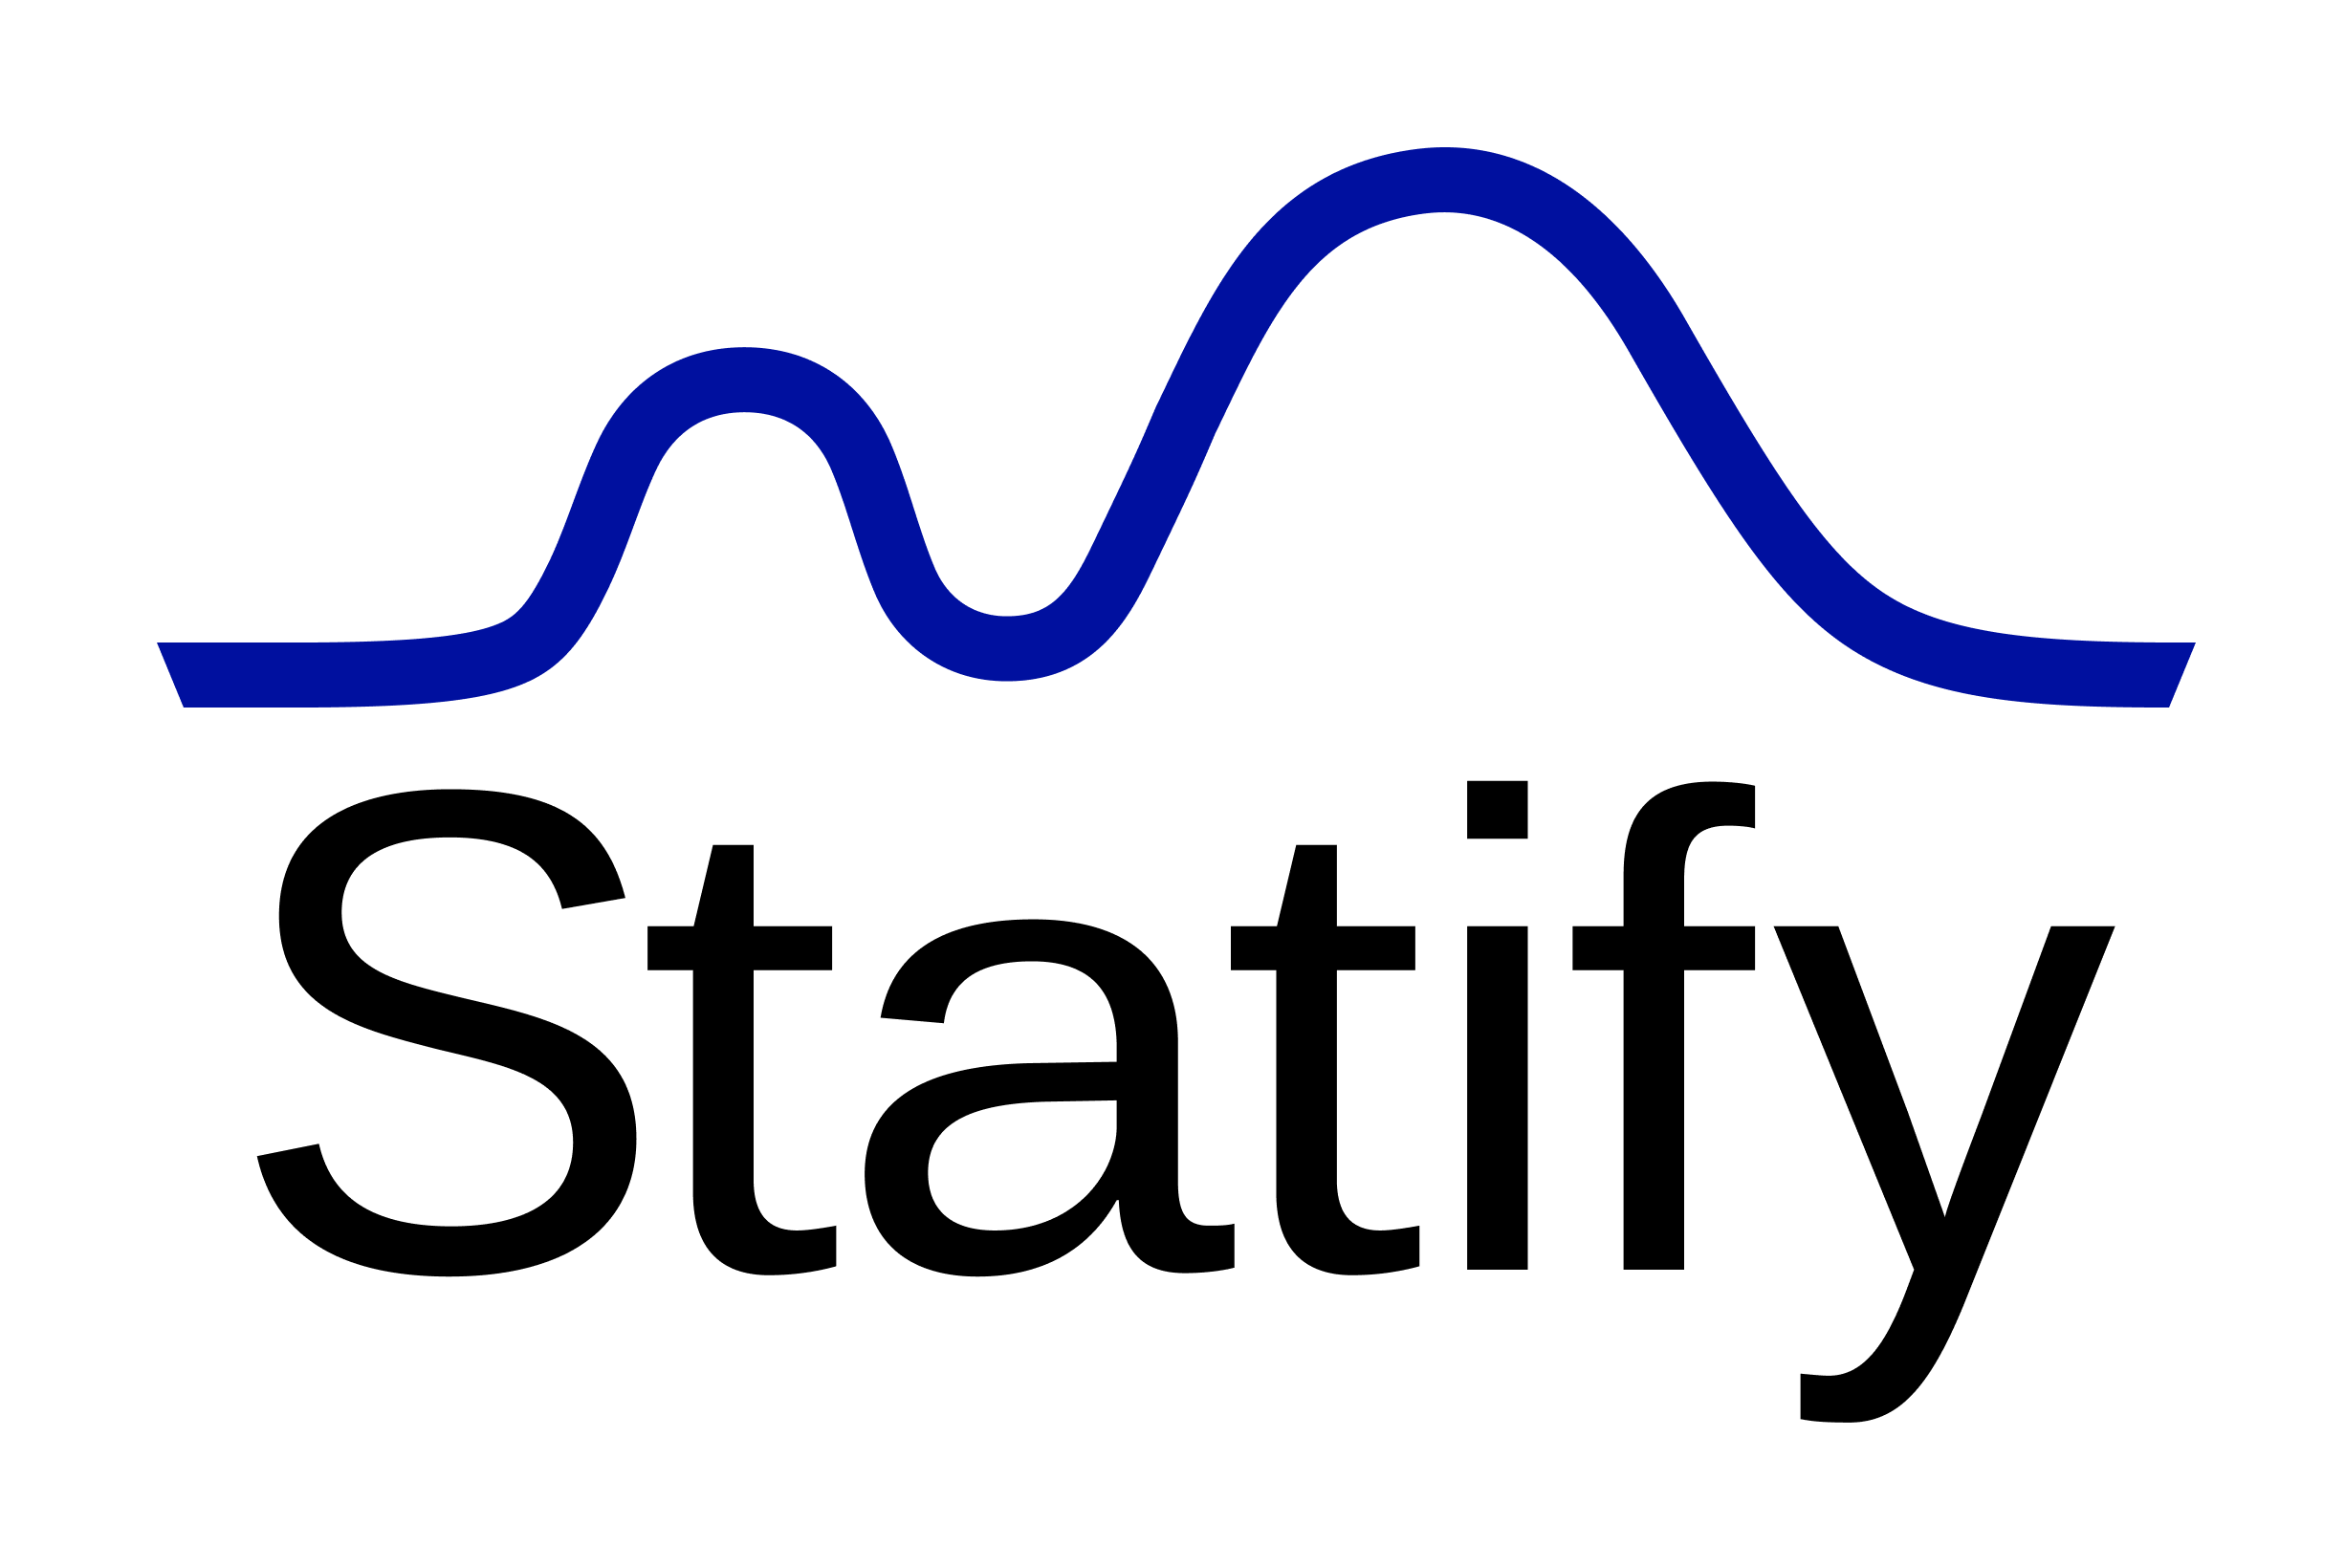
\includegraphics[width=0.3\textwidth]{figures_julyan/logo/statify.png}
}
\date{}



\definecolor{forestgreen}{rgb}{0.13, 0.55, 0.13}
\definecolor{darkblue}{rgb}{0.0, 0.0, 0.65}
\definecolor{violet2}{rgb}{0.5,0,0.5}
\definecolor{orange2}{rgb}{0.8, 0.1, 0.1}       
\definecolor{red2}{rgb}{1, 0.4, 0}






% specifics Julyan
\setlength{\parskip}{0.5\baselineskip}%
\setlength{\parindent}{0pt}%
% end specifics Julyan


\newcommand{\T}{{\text{\tiny\sffamily\upshape\mdseries T}}}
\newcommand{\bx}{\boldsymbol{x}}
\newcommand{\bmu}{\boldsymbol{\mu}}
\newcommand{\bh}{\boldsymbol{h}}
\newcommand{\bb}{\boldsymbol{b}}
\newcommand{\bV}{\boldsymbol{V}}
\newcommand{\bW}{\boldsymbol{W}}
%\newcommand{\bU}{\boldsymbol{U}}
\newcommand{\bH}{\boldsymbol{H}}
\newcommand{\bw}{\boldsymbol{w}}
\newcommand{\bz}{\boldsymbol{z}} 
\newcommand{\bX}{\boldsymbol{X}} 
\newcommand{\by}{\boldsymbol{y}} 
\newcommand{\bg}{\boldsymbol{g}} 
\newcommand{\bv}{\boldsymbol{v}} 
\newcommand{\be}{\boldsymbol{e}} 
\newcommand{\boldf}{\boldsymbol{f}} 
\newcommand{\Lnorm}{\mathcal{L}} 
\newcommand{\R}{\mathbb{L}} 
\newcommand{\subW}{subW} % \normalfont 

\def\simiid{\overset{\text{iid}}{\sim}}
\def\simind{\overset{\text{ind}}{\sim}}
%\newcommand{\ind}{\perp\!\!\!\!\perp} 

% for BNP part

%% Michal's

\newcommand{\PrecisionParam}{\alpha}
\newcommand{\Dir}{\text{Dir}}
\newcommand{\Beta}{\text{Beta}}

\usepackage{mathtools}

\newcommand\diseq{\stackrel{\mathclap{\normalfont\mbox{\small{d}}}}{=}}


%\newcommand{\distas}[1]{\mathbin{\overset{#1}{\kern\z@\sim}}}%
\newsavebox{\mybox}\newsavebox{\mysim}
\newcommand{\distras}[1]{%
  \savebox{\mybox}{\hbox{\kern3pt$\scriptstyle#1$\kern3pt}}%
  \savebox{\mysim}{\hbox{$\sim$}}%
  \mathbin{\overset{#1}{\kern\z@\resizebox{\wd\mybox}{\ht\mysim}{$\sim$}}}%
}


%% mathbb
\newcommand{\bbC}{\mathbb{C}}
\newcommand{\indic}{\mathds{1}}
\newcommand{\F}{\mathbb{F}}
\newcommand{\X}{\mathbb{X}}
%\newcommand{\Z}{\mathbb{Z}}
\newcommand{\Sd}{\mathbb{S}}
\newcommand{\Y}{\mathbb{Y}}


%% mathds
%\newcommand{\R}{\mathbb{R}}
\newcommand{\E}{\mathrm{E}}
\newcommand{\Cov}{\mathsf{Cov}}
\newcommand{\Var}{\mathsf{Var}}
\newcommand{\N}{\mathds{N}}
\newcommand{\Nbb}{\mathds{N}}
\renewcommand{\P}{\mathds{P}}

\newcommand{\Xn}{X^n}



%%% Script letters
\newcommand{\Bcr}{\mathscr{B}}
\newcommand{\Fcr}{\mathscr{F}}
\newcommand{\Dcr}{\mathscr{D}}
\newcommand{\Icr}{\mathscr{I}}
\newcommand{\Lcr}{\mathscr{L}}
\newcommand{\Pcr}{\mathscr{P}}
\newcommand{\Xcr}{\mathscr{X}}
\newcommand{\Mcr}{\mathscr{M}}
\newcommand{\Ycr}{\mathscr{Y}}
\newcommand{\Acr}{\mathscr{A}}
\newcommand{\Gcr}{\mathscr{G}}
\newcommand{\Vcr}{\mathscr{V}}

%%% Mathfrak
\newcommand{\Xf}{\mathfrak{X}}
\newcommand{\Sf}{\mathfrak{\sigma}}

\newcommand{\ddr}{\mathrm{d}}
\newcommand{\edr}{\mathrm{e}}
\newcommand{\idr}{\mathrm{i}}

%\renewcommand{\abstractname}{SUMMARY}
\renewcommand{\theparagraph}{\arabic{paragraph}}
%\numberwithin{equation}{paragraph}

\newcommand{\Rt}{\Rightarrow}
\newcommand{\rt}{\rightarrow}
\newcommand{\lrt}{\longrightarrow}
\newcommand{\Lerit}{\Leftrightarrow}
\newcommand{\dimo}{\underline{\textsc{Proof.}} }
\newcommand{\cc}{\hfill $\square$}
\newcommand{\ind}{\bm 1}
\newcommand{\bm}{\mathbf}
\newcommand{\var}{\varepsilon}
\newcommand{\intre}{\int_{\mathbb{R}}}
\newcommand{\intoinf}{\int_0^{+\infty}}

\newcommand{\Bc}{\mathcal{B}}
\newcommand{\Cc}{\mathcal{C}}
\newcommand{\Fc}{\mathcal{F}}
\newcommand{\Lc}{\mathcal{L}}
\newcommand{\Nc}{\mathcal{N}}
\newcommand{\Pc}{\mathcal{P}}
\newcommand{\Ic}{\mathcal{I}}
\newcommand{\Zc}{\mathcal{Z}}

\newcommand{\dir}{P_{\alpha}}
\newcommand{\ep}{\varepsilon}
\newcommand{\e}{\mathsf{E}}
\newcommand{\trunc}{{\sigma,\tau}}
%\newcommand{\p}{\mathbb{P}}
\newcommand{\prob}{\mathsf{P}}
\newcommand{\Ga}{\Gamma_\alpha}
\newcommand{\Ma}{M_\alpha}
\newcommand{\Ua}{U_\alpha}
\newcommand{\Va}{V_\alpha}
\newcommand{\wt}{\widetilde}

\def\simind{\stackrel{\mbox{\scriptsize{ind}}}{\sim}}
\def\simiid{\stackrel{\mbox{\scriptsize{iid}}}{\sim}}

% altro
\newcommand{\mt}{{\mu}} % misura completamente aleatoria (CRM)
\newcommand{\hti}{{h}}
\newcommand{\St}{{S}}
\newcommand{\pt}{\tilde{p}} % legge aleatoria
\newcommand{\At}{\tilde{A}} %
\newcommand{\Bt}{\tilde{B}} %
\newcommand{\Lz}{\mathcal{L}_Z} % legge di Z

\newcommand{\AC}{\\[7pt]} % a capo
\newcommand{\La}{\mathcal{L}}
%\newcommand{\p}{\mathbb{P}}
%\newcommand{\AC}{\\[7pt]}
\newcommand{\bn}{\bar{n}}
\newcommand{\I}{\mathcal{I}}
\newcommand{\C}{\mathcal{C}}
\newcommand{\Ac}{\mathcal{A}}

% Ju
\newcommand{\vertju}{\,\vert\,}
\newcommand{\twoPD}{two-parameter Poisson-Dirichlet process\xspace}
\newcommand{\DP}{\text{Dirichlet process}\xspace}
\newcommand{\levy}{L\'evy\xspace}
\newcommand{\Gumbel}{\text{Gumbel}\xspace}
\newcommand{\Exp}{\text{Exp}\xspace}
\def\simiid{\stackrel{\mbox{\scriptsize{iid}}}{\sim}}
\def\simind{\stackrel{\mbox{\scriptsize{ind}}}{\sim}}
\def\proptoind{\stackrel{\mbox{\scriptsize{ind}}}{\propto}}
\newcommand{\citp}[1]{\textcolor{blue}{\citep{#1}}}
\newcommand{\citt}[1]{\textcolor{blue}{\citet{#1}}}


\newcommand{\crms}{completely random measures\xspace}
\newcommand{\crm}{completely random measure\xspace}
\newcommand{\CRM}{CRM\xspace}
\newcommand{\Crms}{Completely random measures\xspace}
\newcommand{\Crm}{Completely random measure\xspace}
\newcommand{\muA}{\tilde \mu(A)\xspace}
\newcommand{\muX}{\tilde \mu(\X)\xspace}
\newcommand{\cnkpar}{\binom{n}{k_1\cdots k_n}}
\newcommand{\cnkfact}{\frac{n!}{k_1!\ldots k_n!}}
\newcommand{\g}{\mathbf{g}}
\newcommand{\FK}{\citeauthor{ferguson1972representation}\xspace} 
\newcommand{\FKa}{\citeauthor{ferguson1972representation} algorithm\xspace} 
\newcommand{\BP}{\ensuremath{\text{BP}}\xspace} 
\newcommand{\BeP}{\ensuremath{\text{BeP}}\xspace} 
%\newcommand{\gg}{\ensuremath{\text{GG}}\xspace} 
\newcommand{\GG}{generalized gamma process\xspace} 
\newcommand{\SBP}{stable-beta process\xspace} 
\newcommand{\IBP}{Indian buffet process\xspace} 
\newcommand{\IG}{inverse-Gaussian process\xspace} 
\newcommand{\NMC}{N_{\text{\tiny{FK}}}} 
\newcommand{\EFK}{\mathbb{E}_{\text{\tiny{FK}}}}


\def\unit{\mathbf{1}}
\def\bc{c}
\def\prob{\mathbb{P}}
\def\bc{c}
\def\Ac{\mathcal{A}}
\def\VI{\text{VI}}
\def\En{\text{H}}
\def\B{\text{B}}
%\def\argmax{\text{argmax}}
\DeclareMathOperator*{\argmax}{arg\,max}
\DeclareMathOperator*{\argmin}{arg\,min}
\def\1{\unit}




\begin{document}

\begin{frame}[plain]
  \titlepage
\end{frame}

\begin{frame}{Outline}
	\tableofcontents[pausesections,subsectionstyle=hide,subsubsectionstyle=hide]
\end{frame}

%\section[P vs NP]{Motivations to go nonparametric}

\begin{frame}{Parametric versus nonparametric}
 
\begin{block}{Parametric models}
\begin{itemize}
	\item Finite and fixed number of parameters  
	\item Number of parameters is independent of the dataset
\end{itemize}
\end{block}

\begin{block}{Nonparametric models}
	\begin{itemize}
		\item Do have parameters
		\item Can be understood as having an infinite number of  parameters 
		\item Can be understood as having a random number of  parameters
		\item Number of parameters can grow with the dataset
	\end{itemize}
\end{block}
\end{frame}



%%%%%%%%%%%%%%%%%%%%%%%%%%%%%%%%%%%%%%%%%%%%%%%%%%%%%%%%%%%%%%%%%%%%%%%%%%%%%%%%%%%%%%%%%%%%%%%%%%%%%%
\frame{\frametitle{Underlying function}
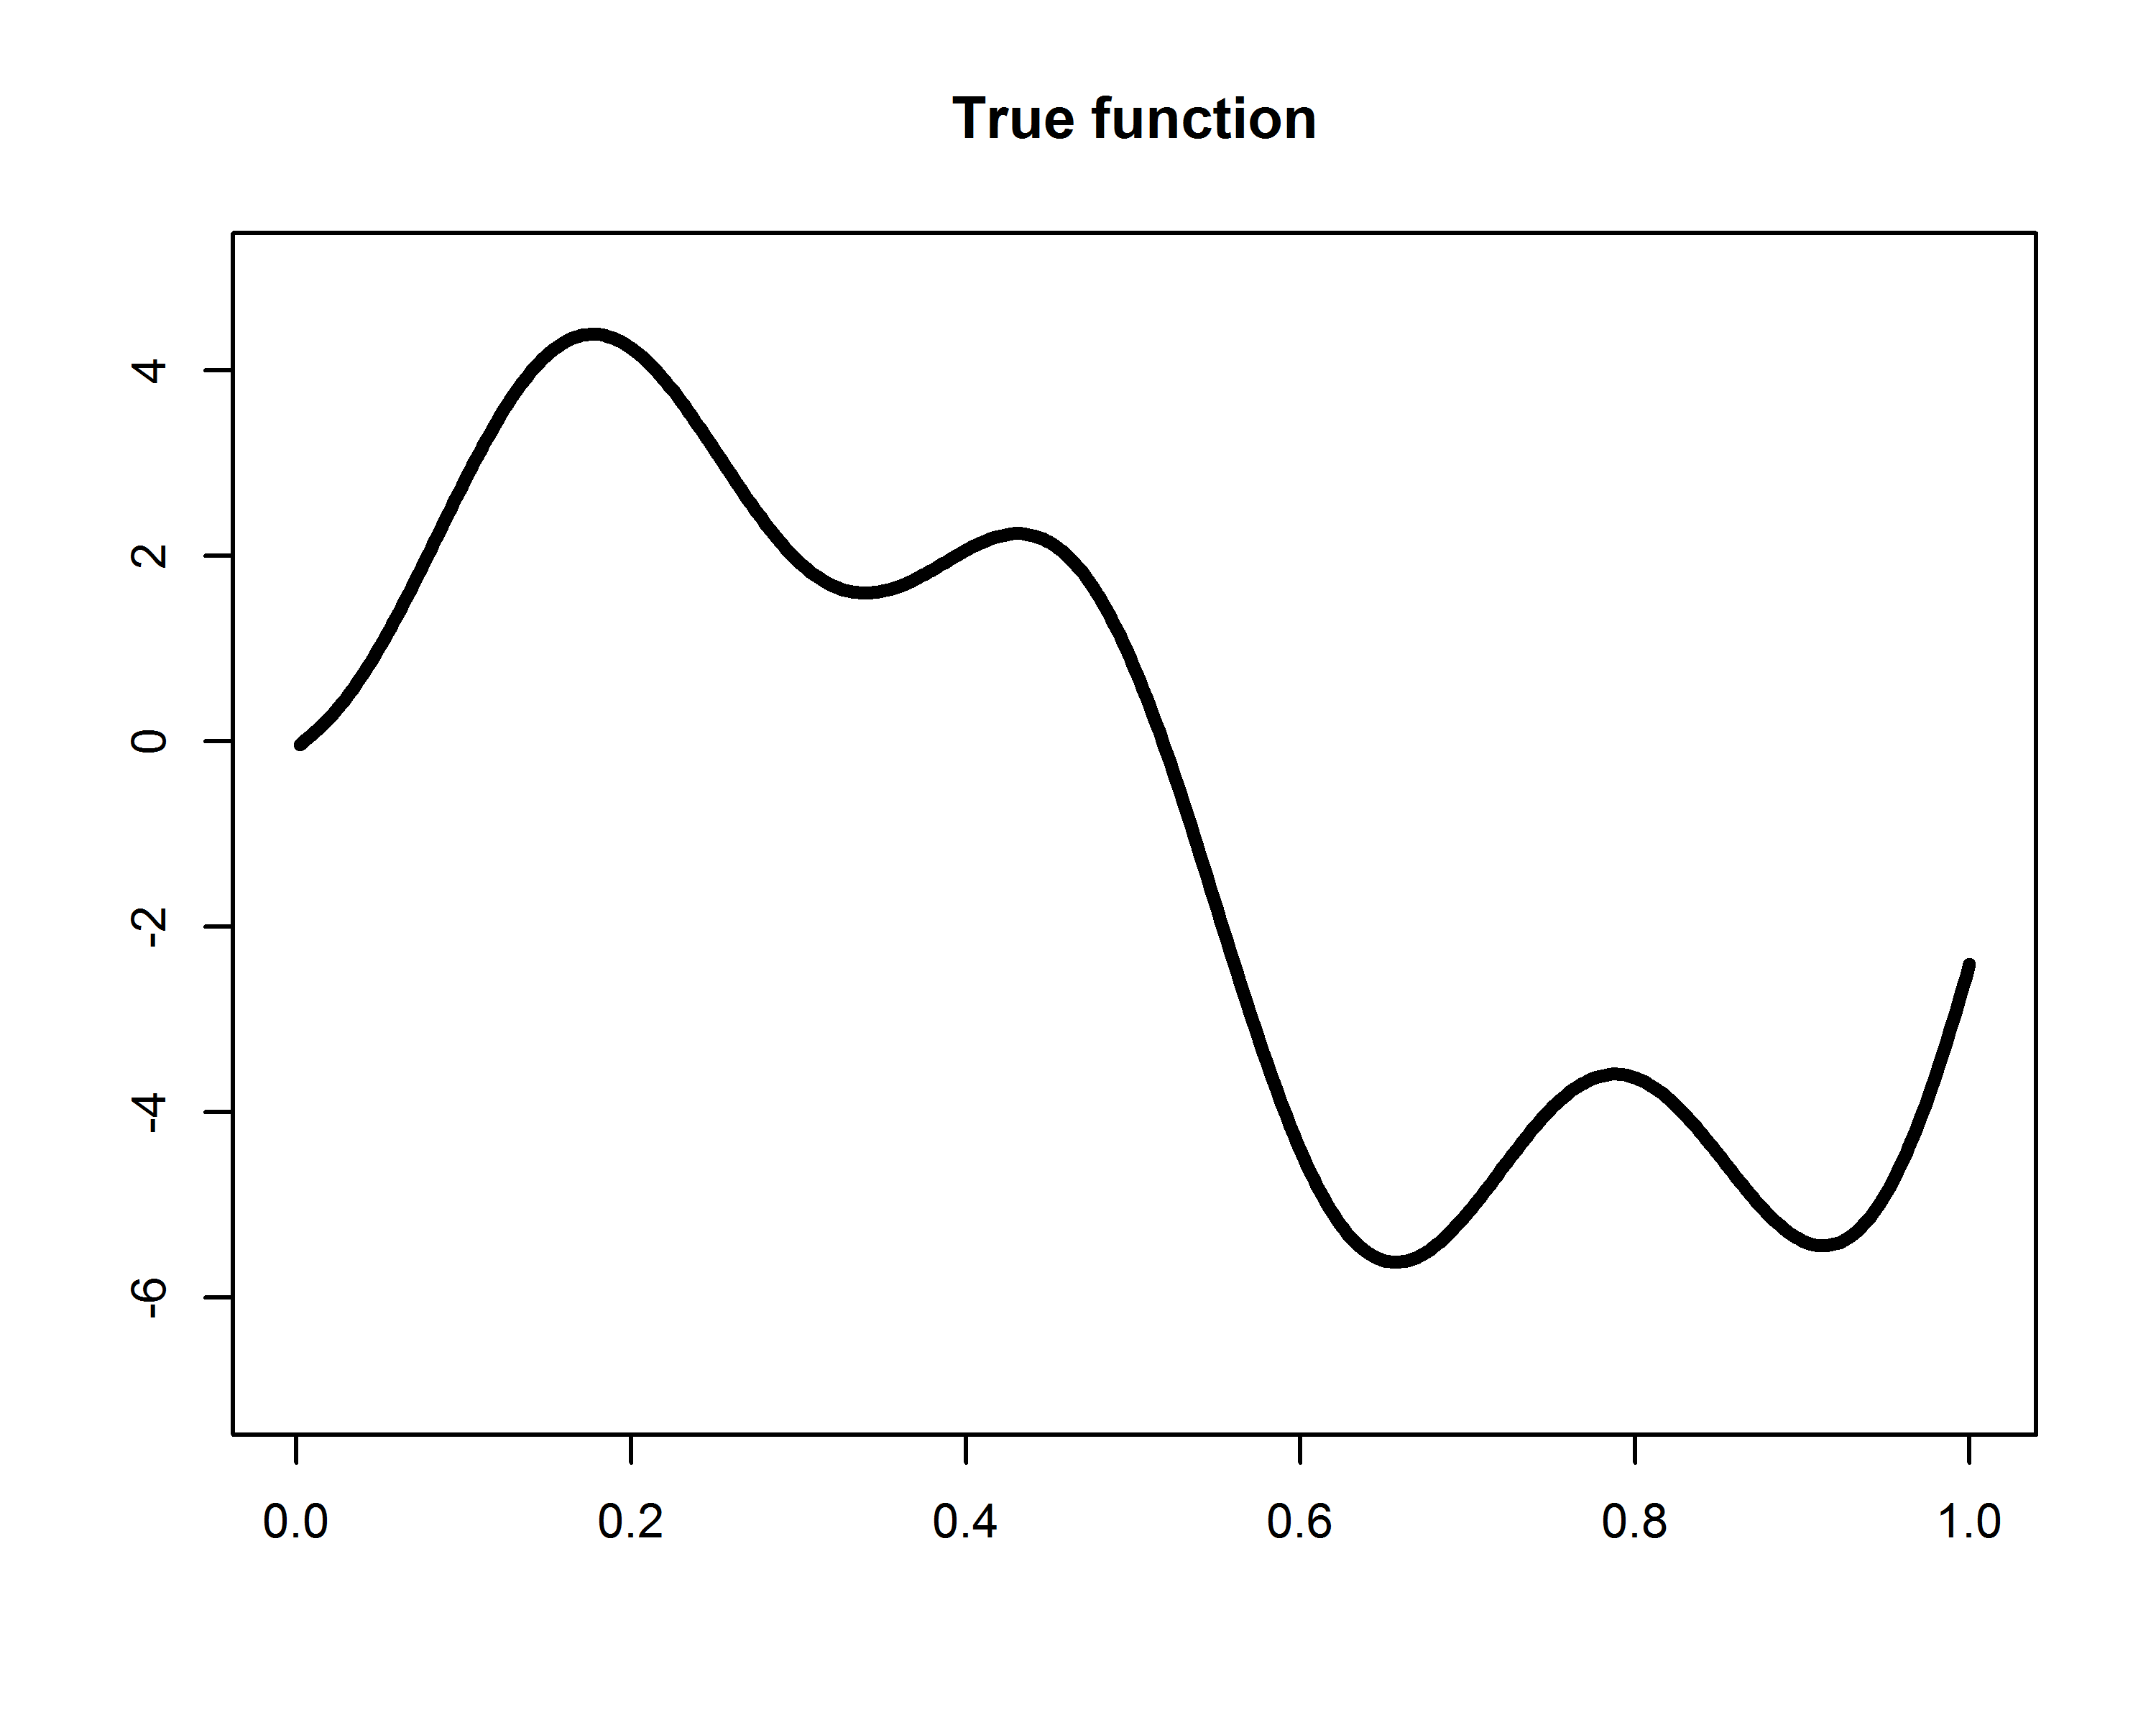
\includegraphics[width = 4in]{figures_julyan/Botond/true.png}
}


\frame{\frametitle{Data}
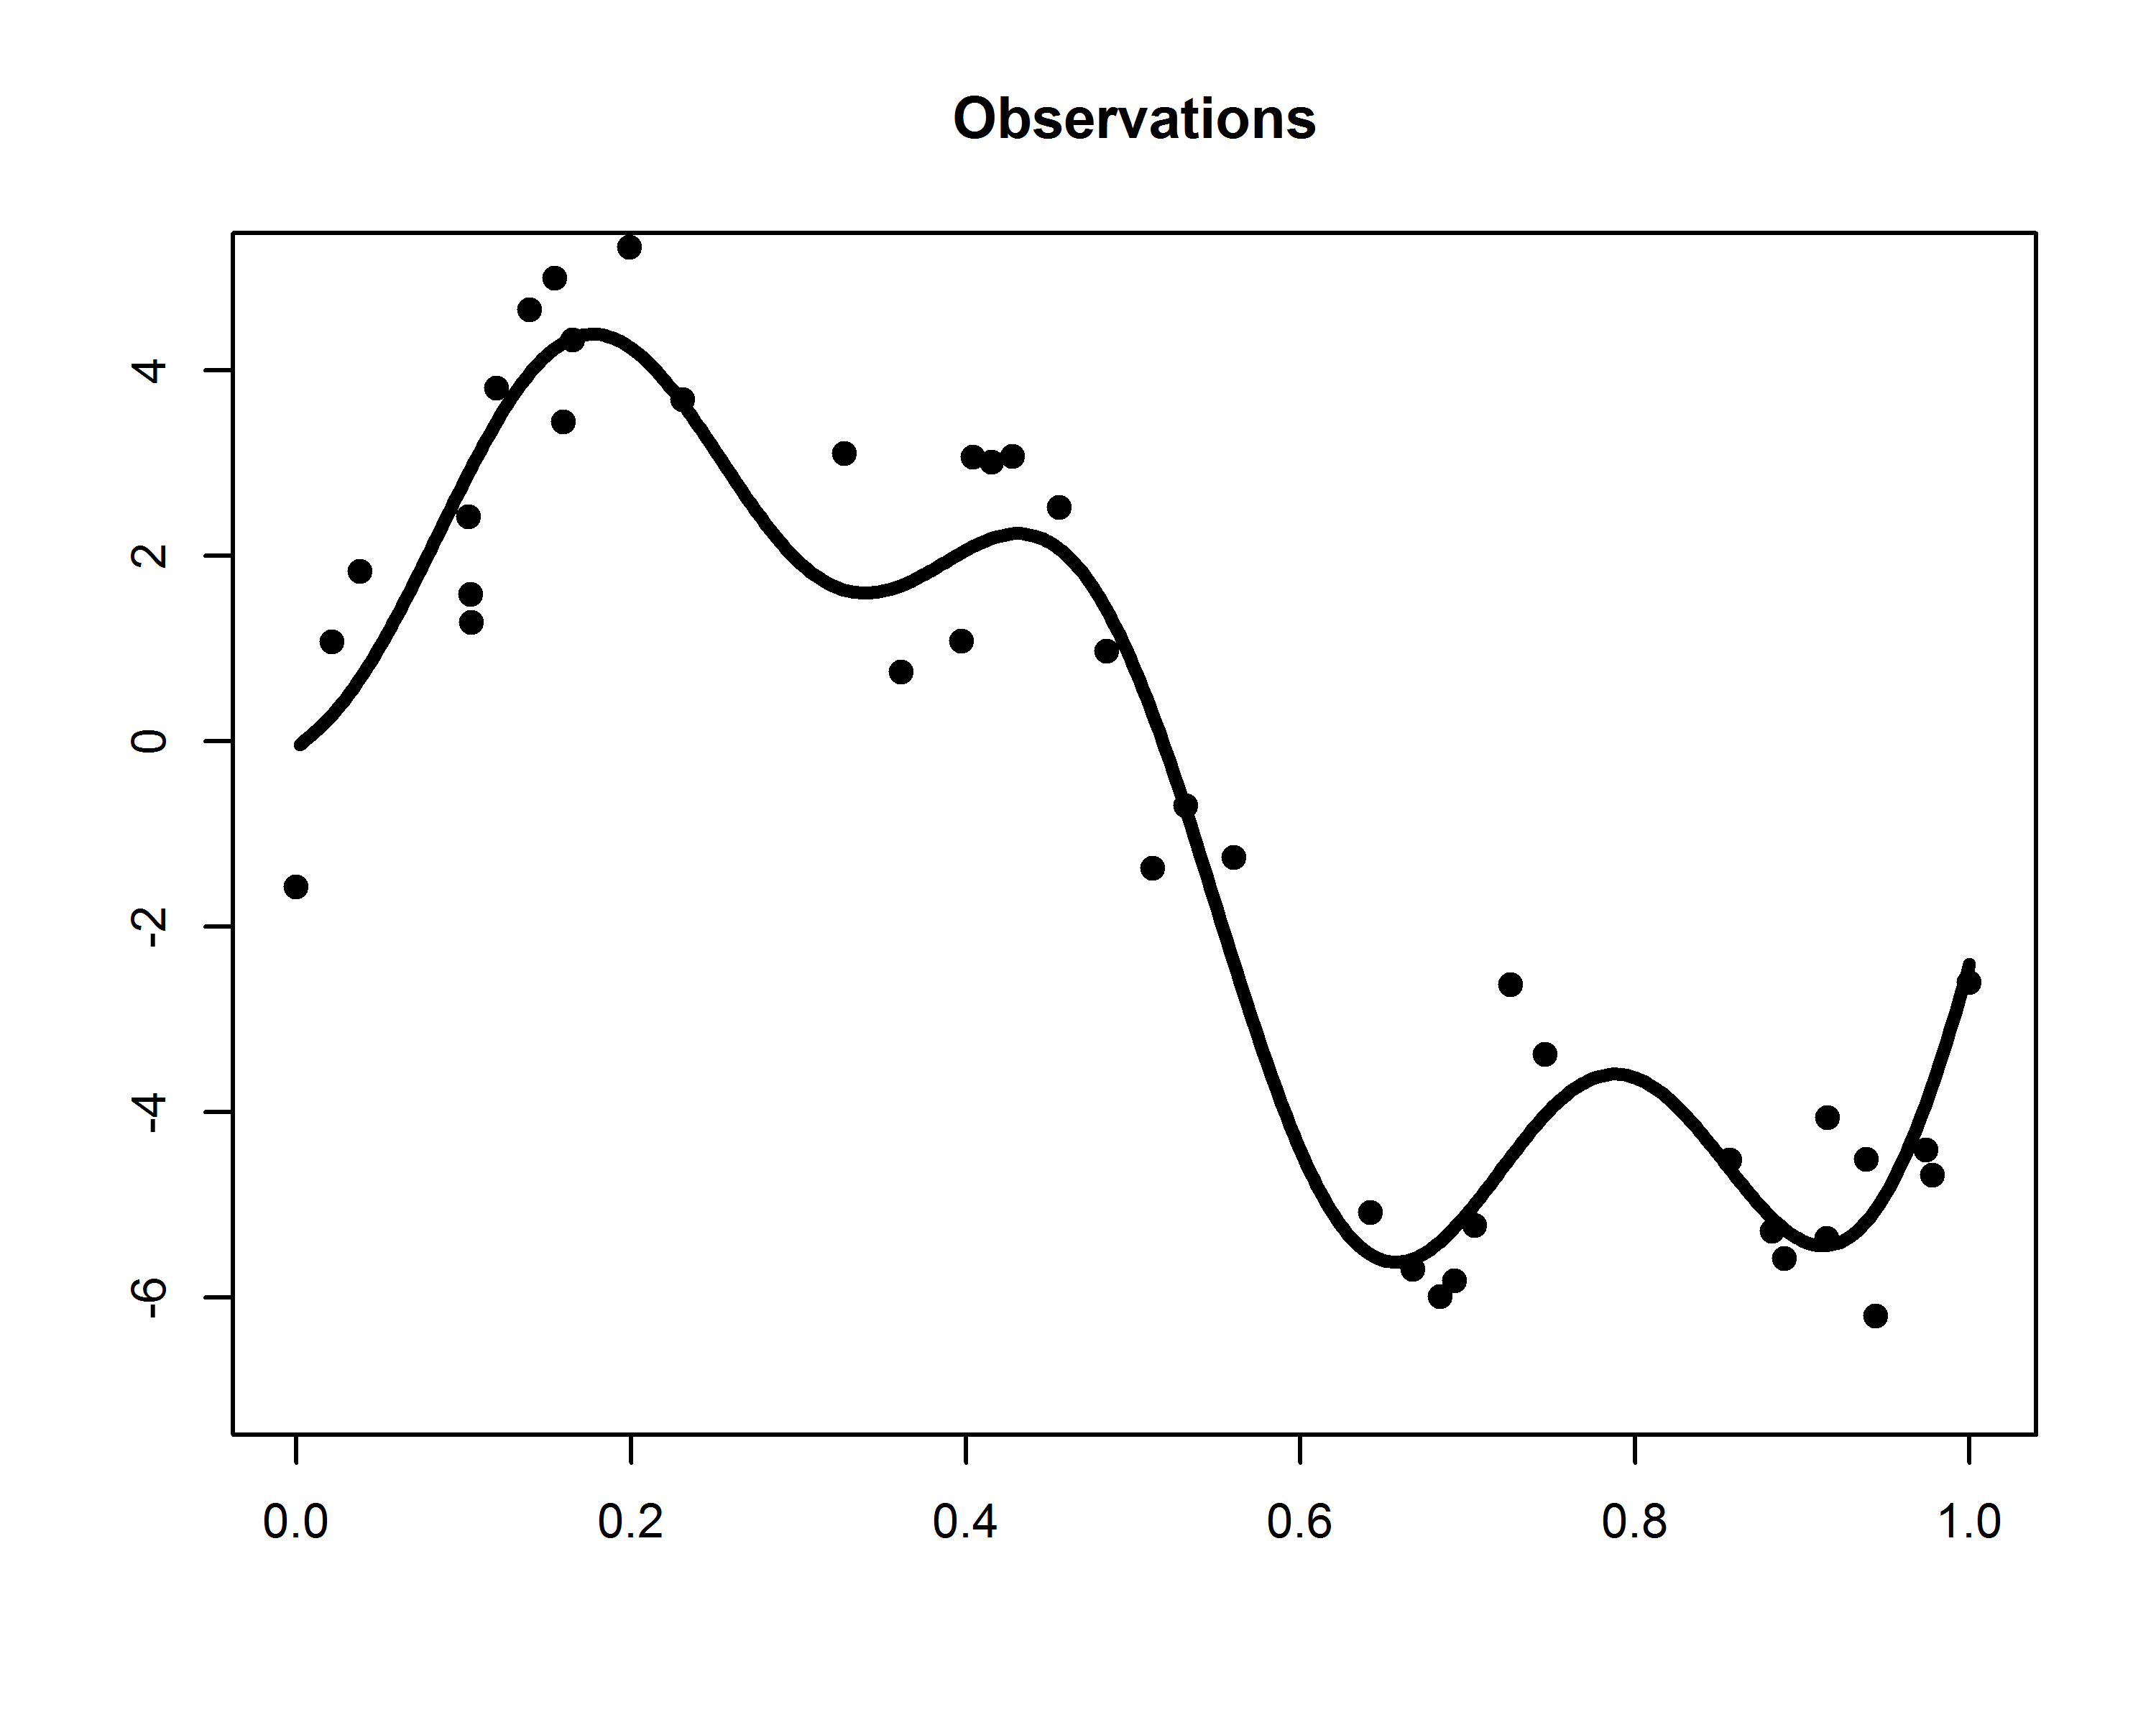
\includegraphics[width = 4in]{figures_julyan/Botond/TrueData2.png}
}


\frame{\frametitle{Parametric fitting}
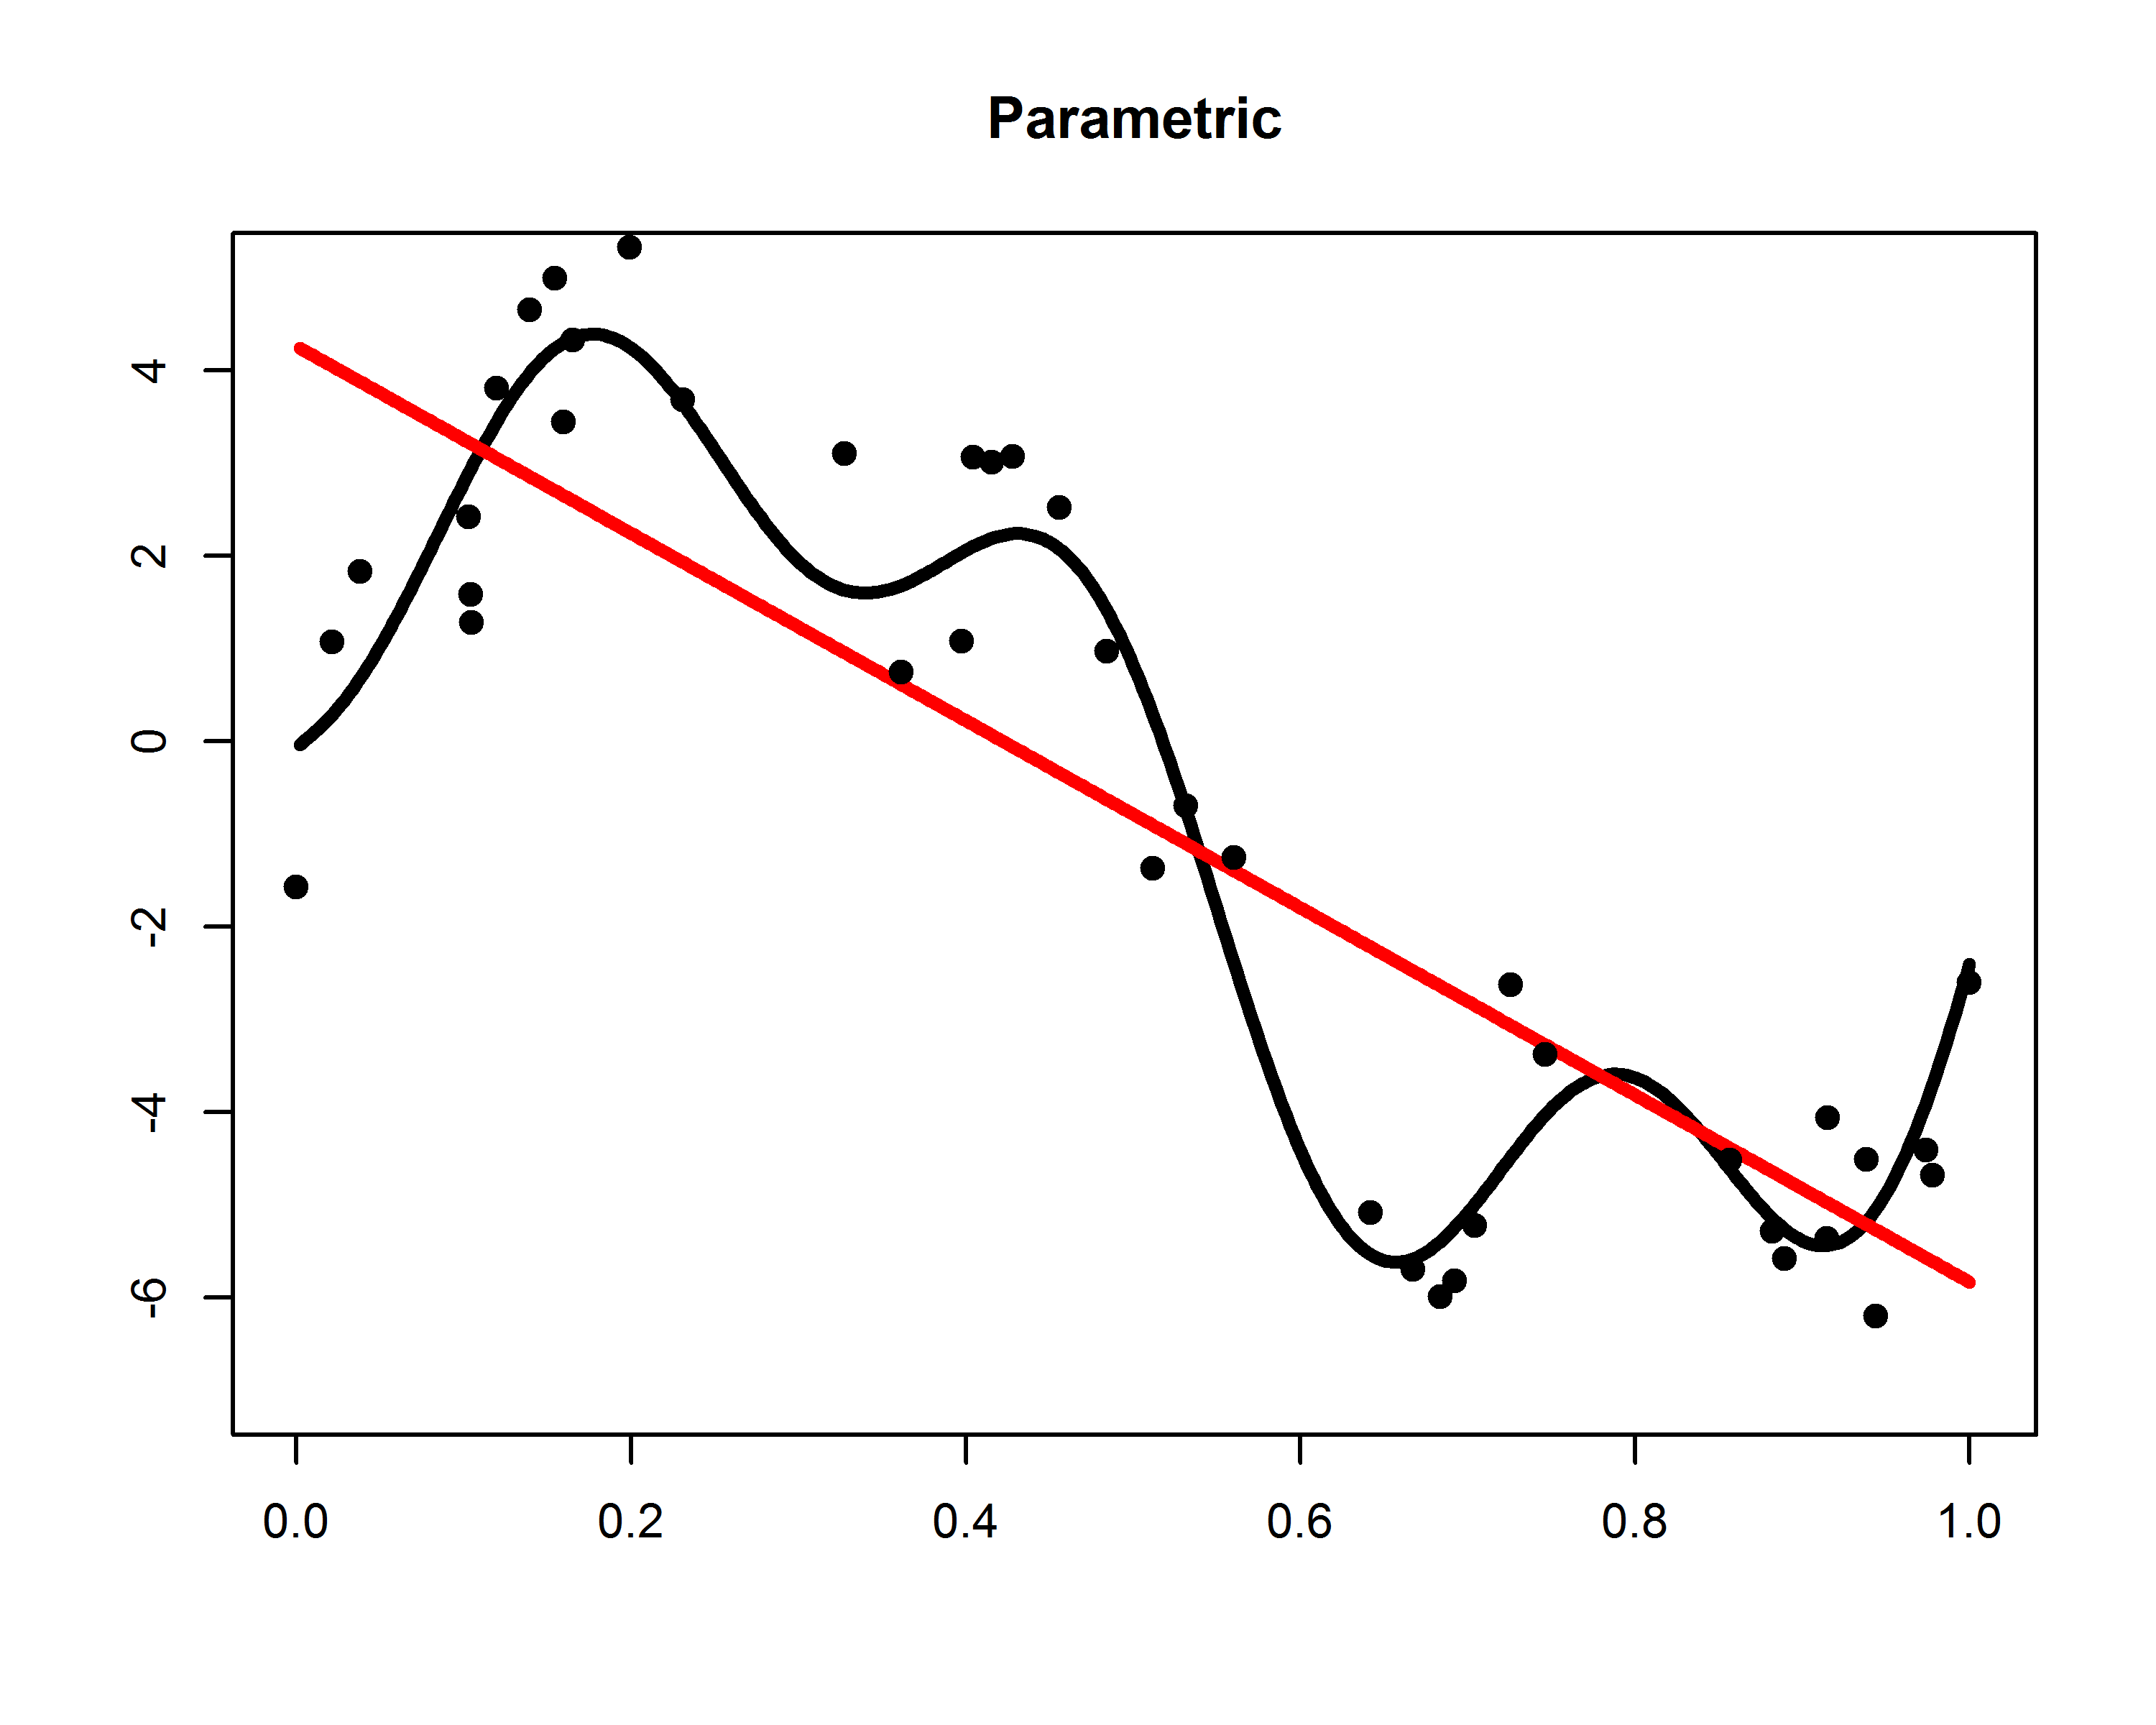
\includegraphics[width = 4in]{figures_julyan/Botond/Parametric.png}
}


\frame{\frametitle{Nonparametric fitting}
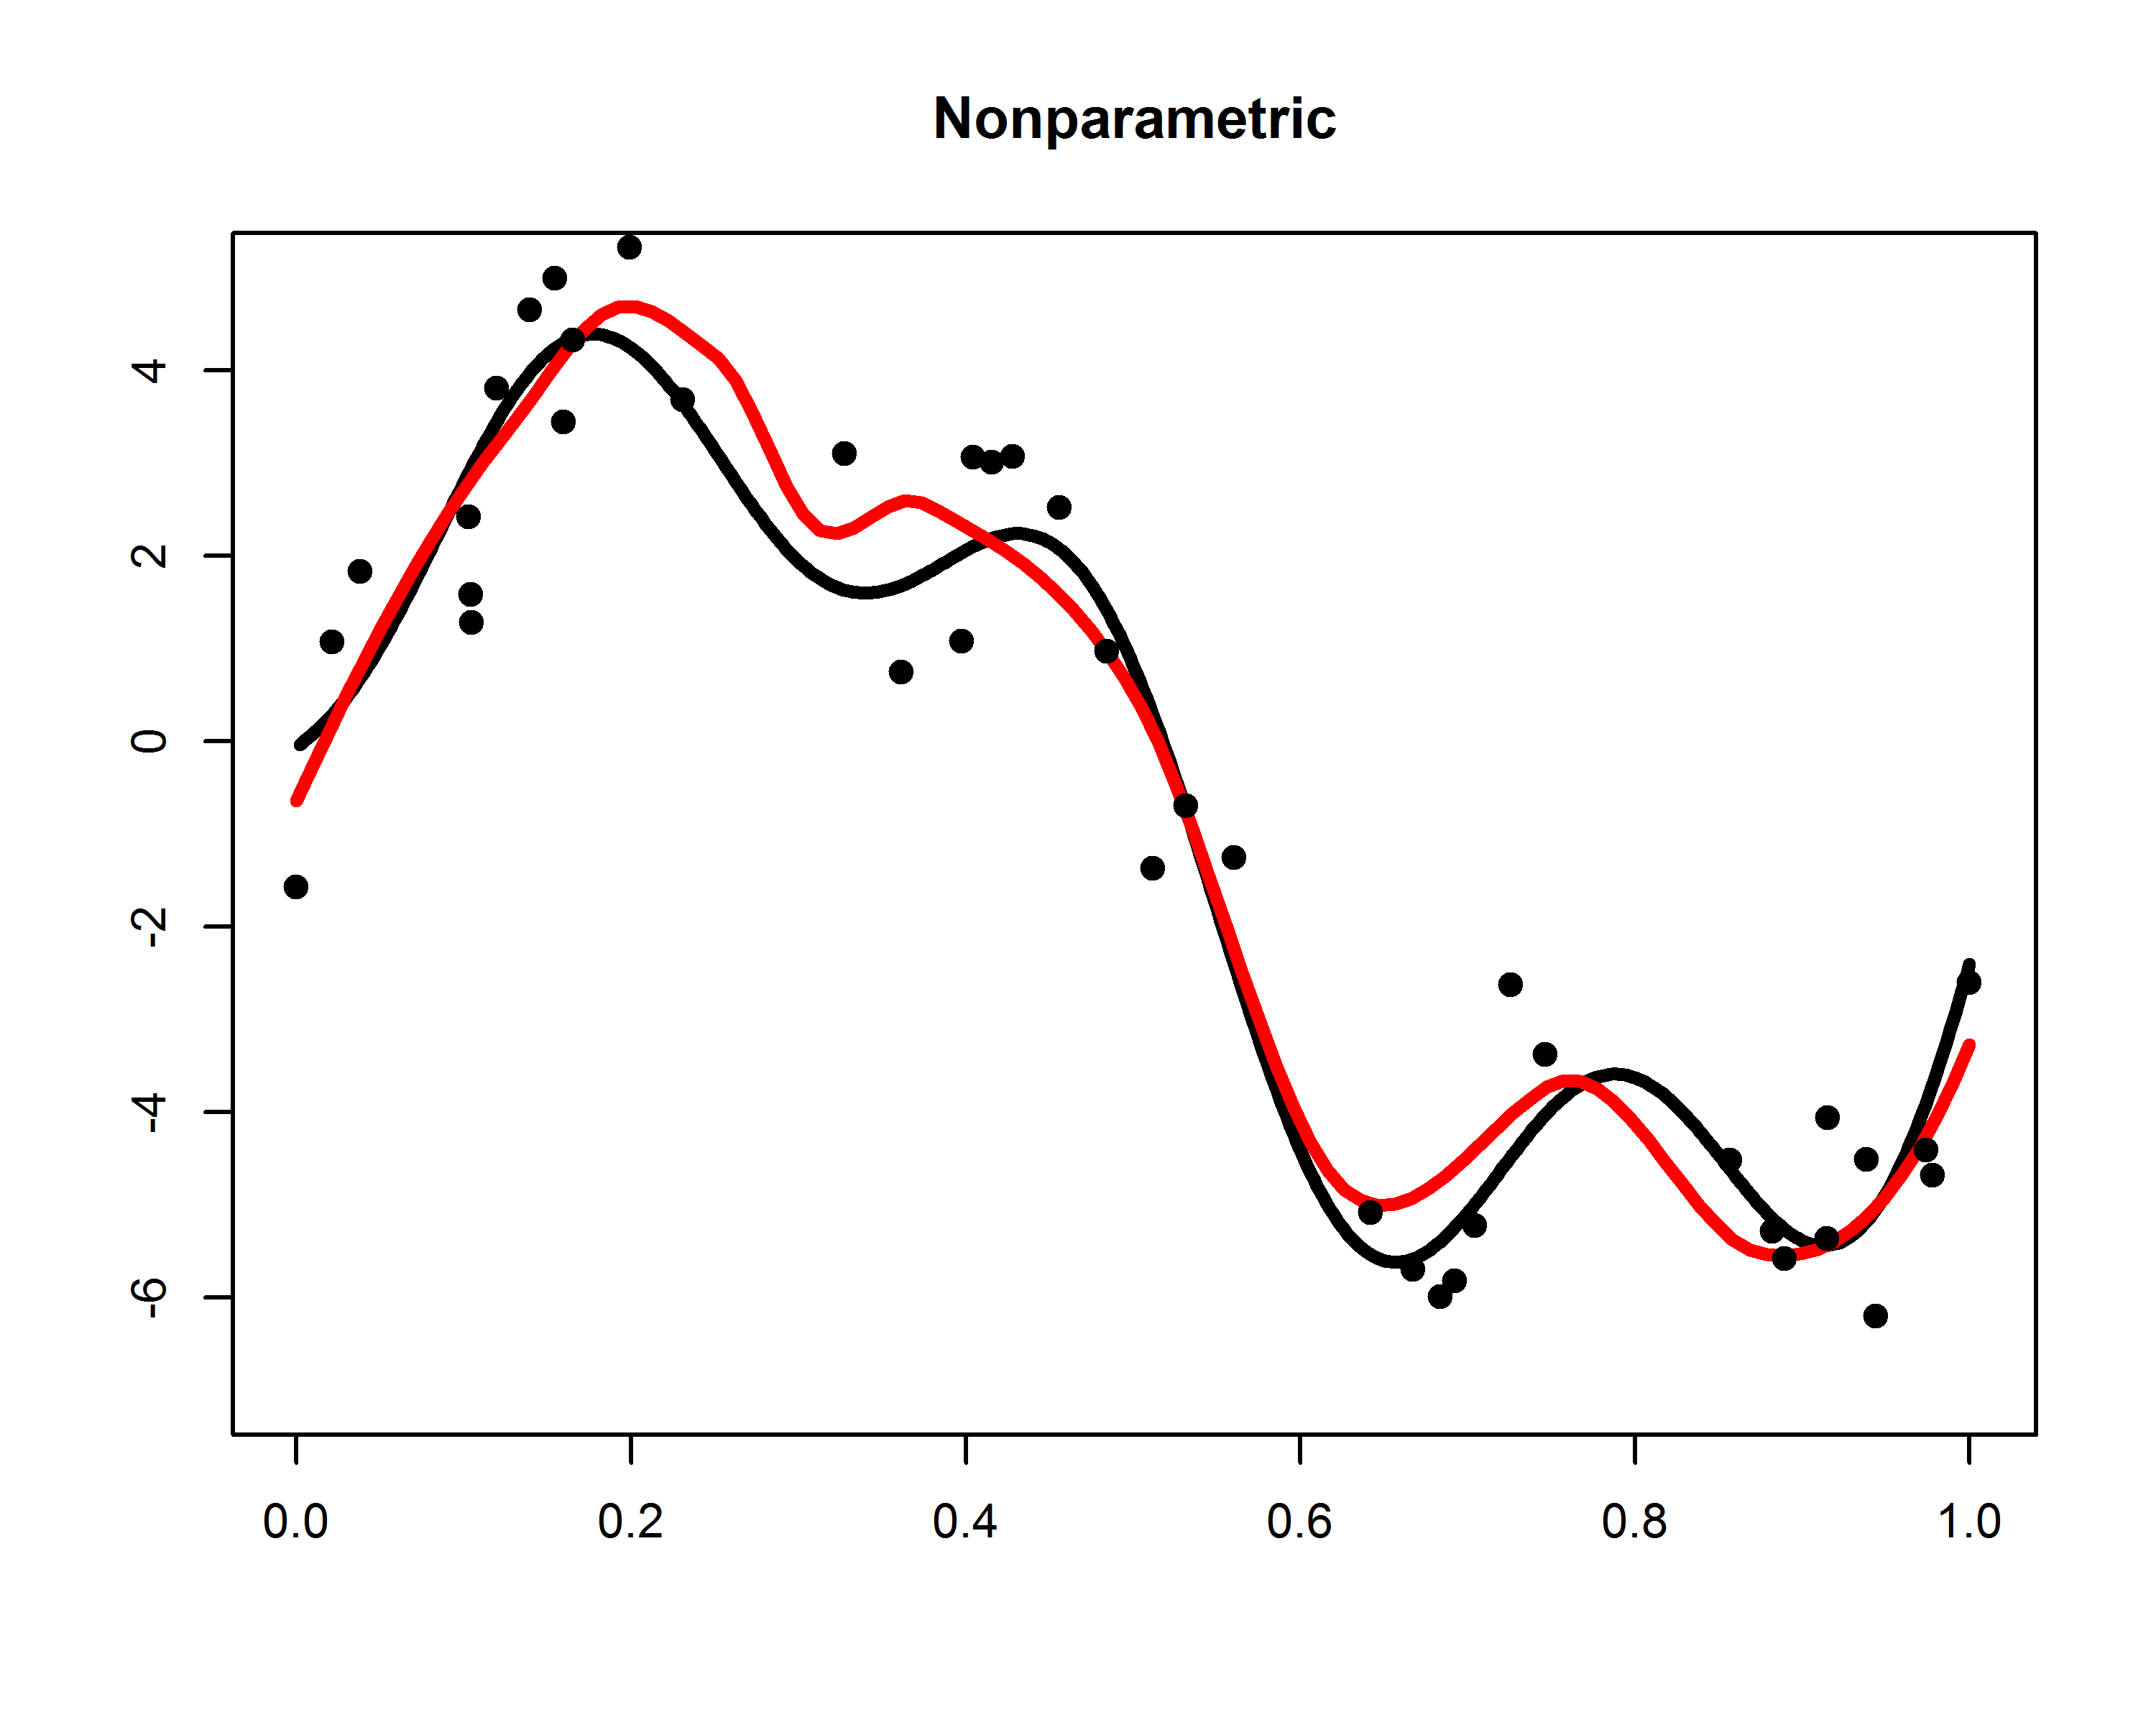
\includegraphics[width = 4in]{figures_julyan/Botond/NP.png}\vspace{-0.3cm}\\
}


\frame{\frametitle{Prior}
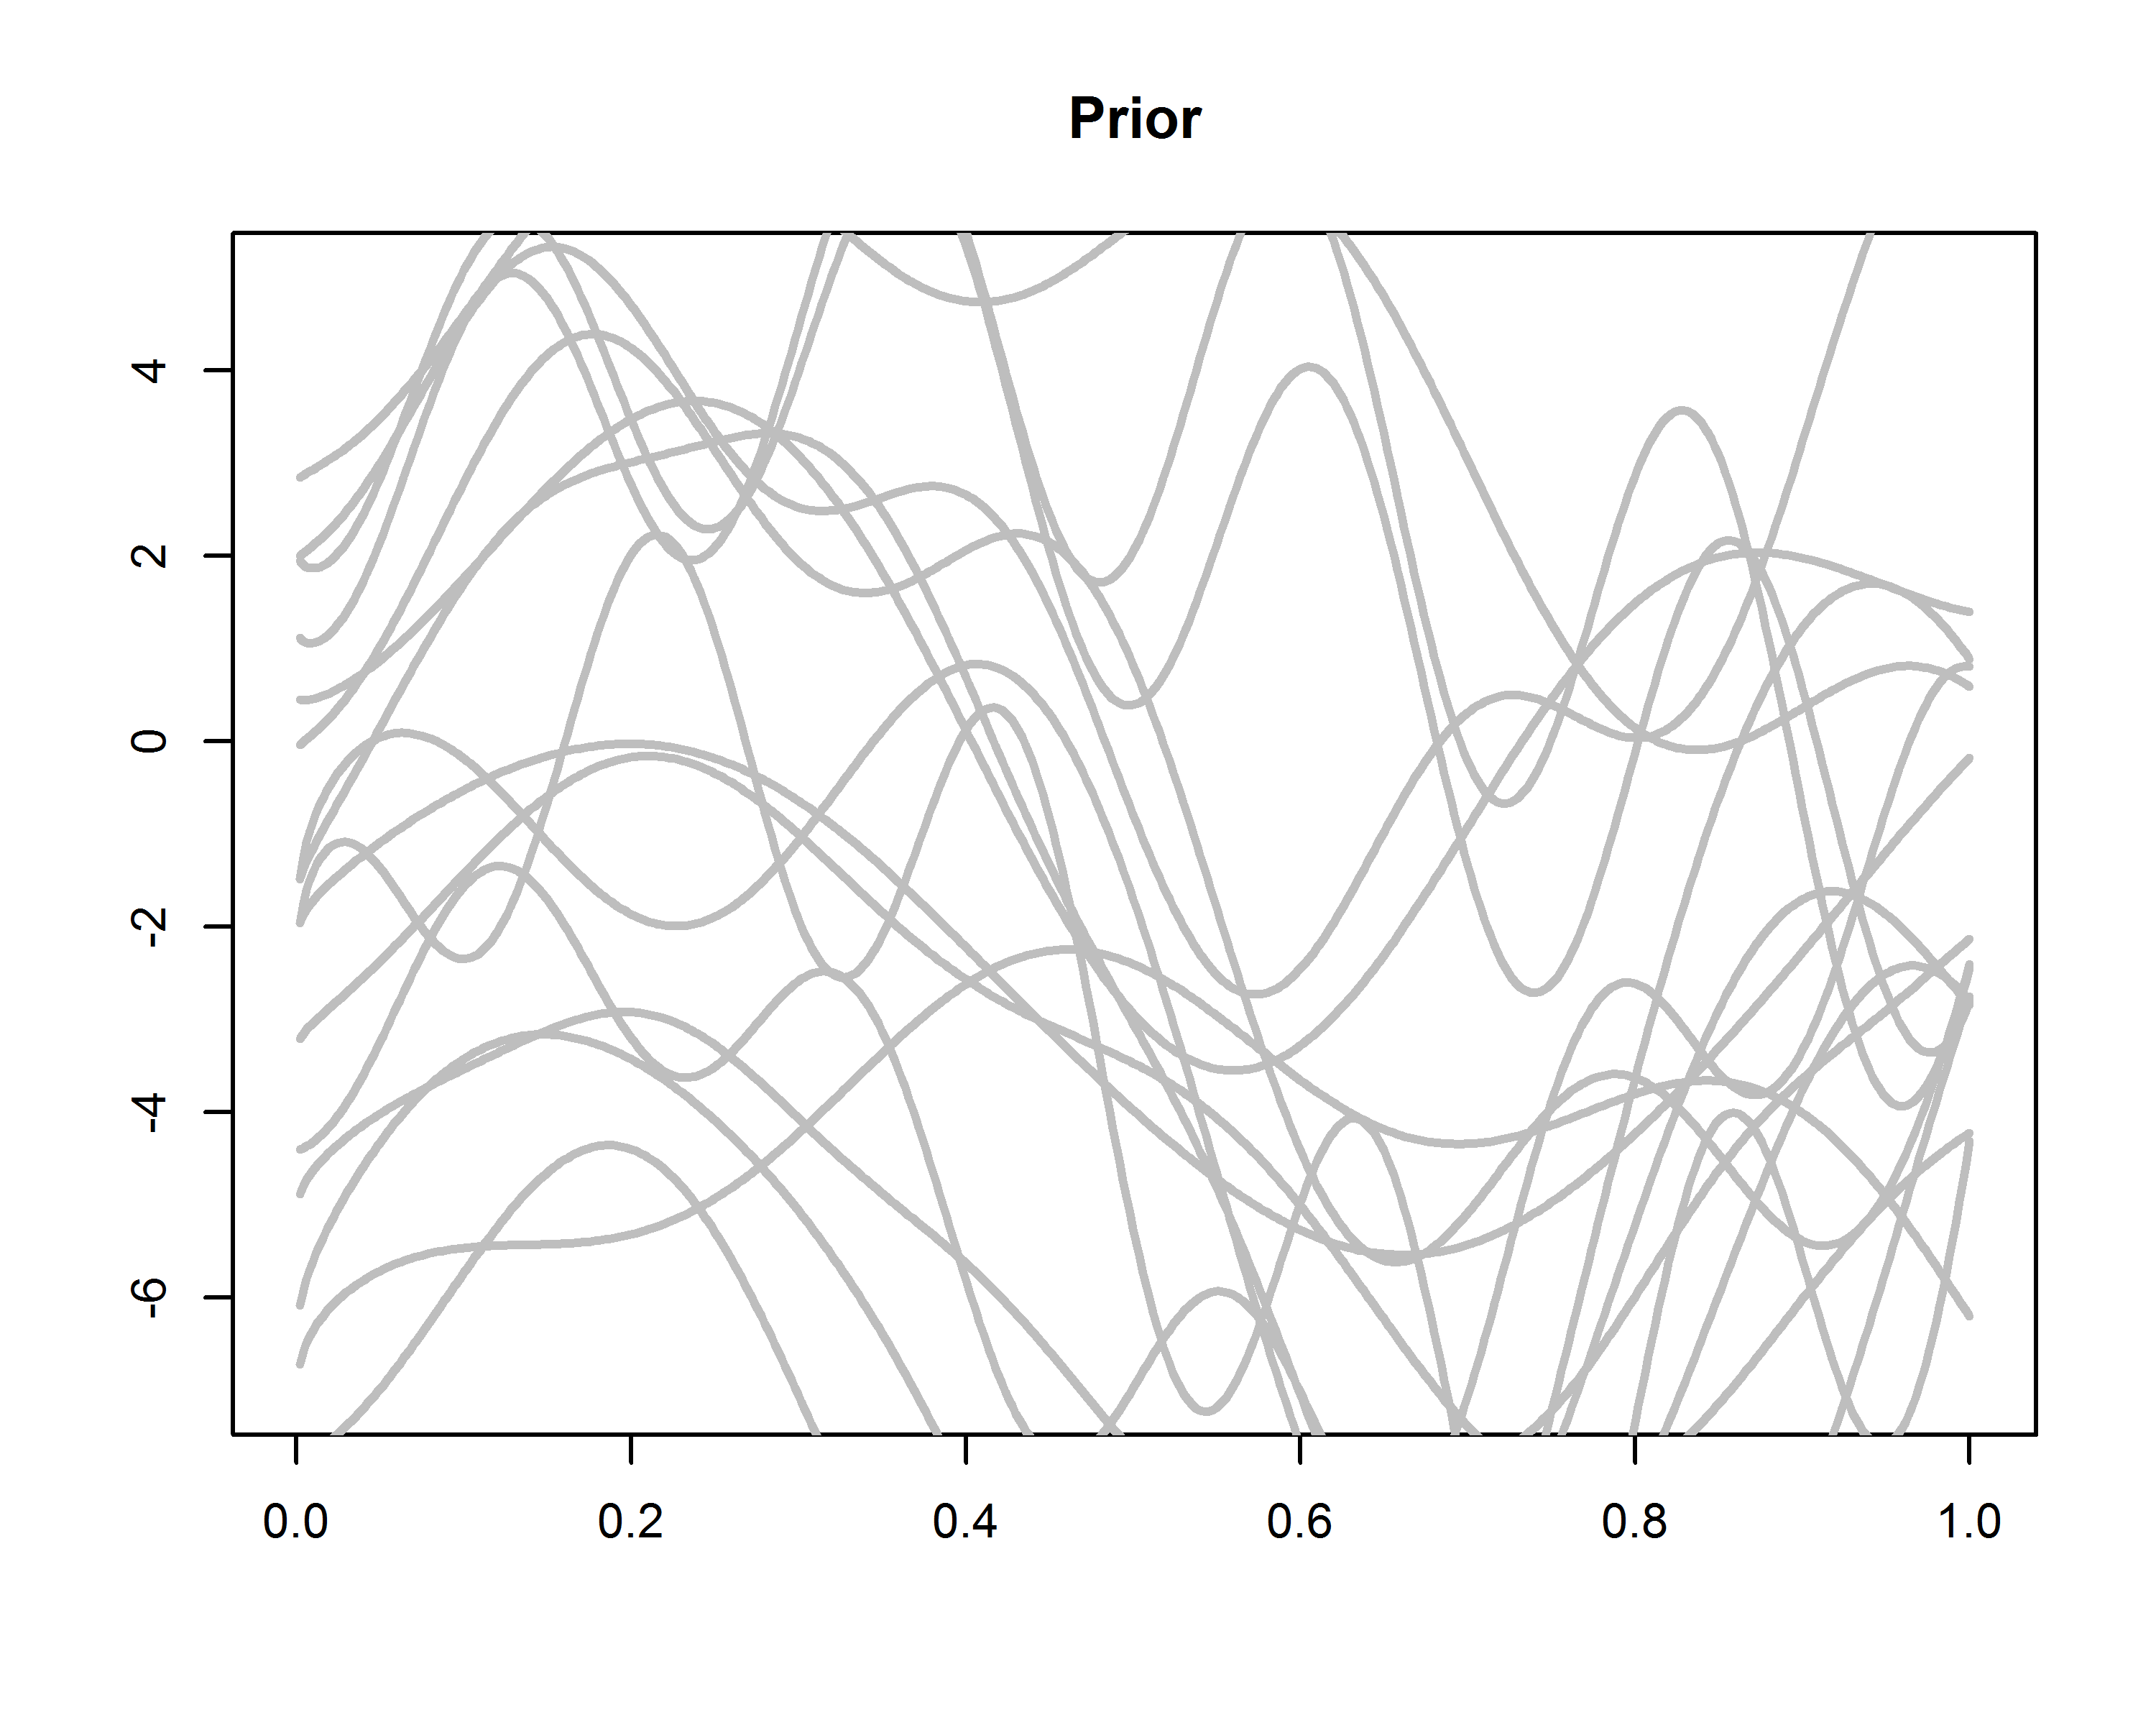
\includegraphics[width = 4in]{figures_julyan/Botond/Prior.png}\vspace{-0.3cm}\\
}


\frame{\frametitle{Posterior}
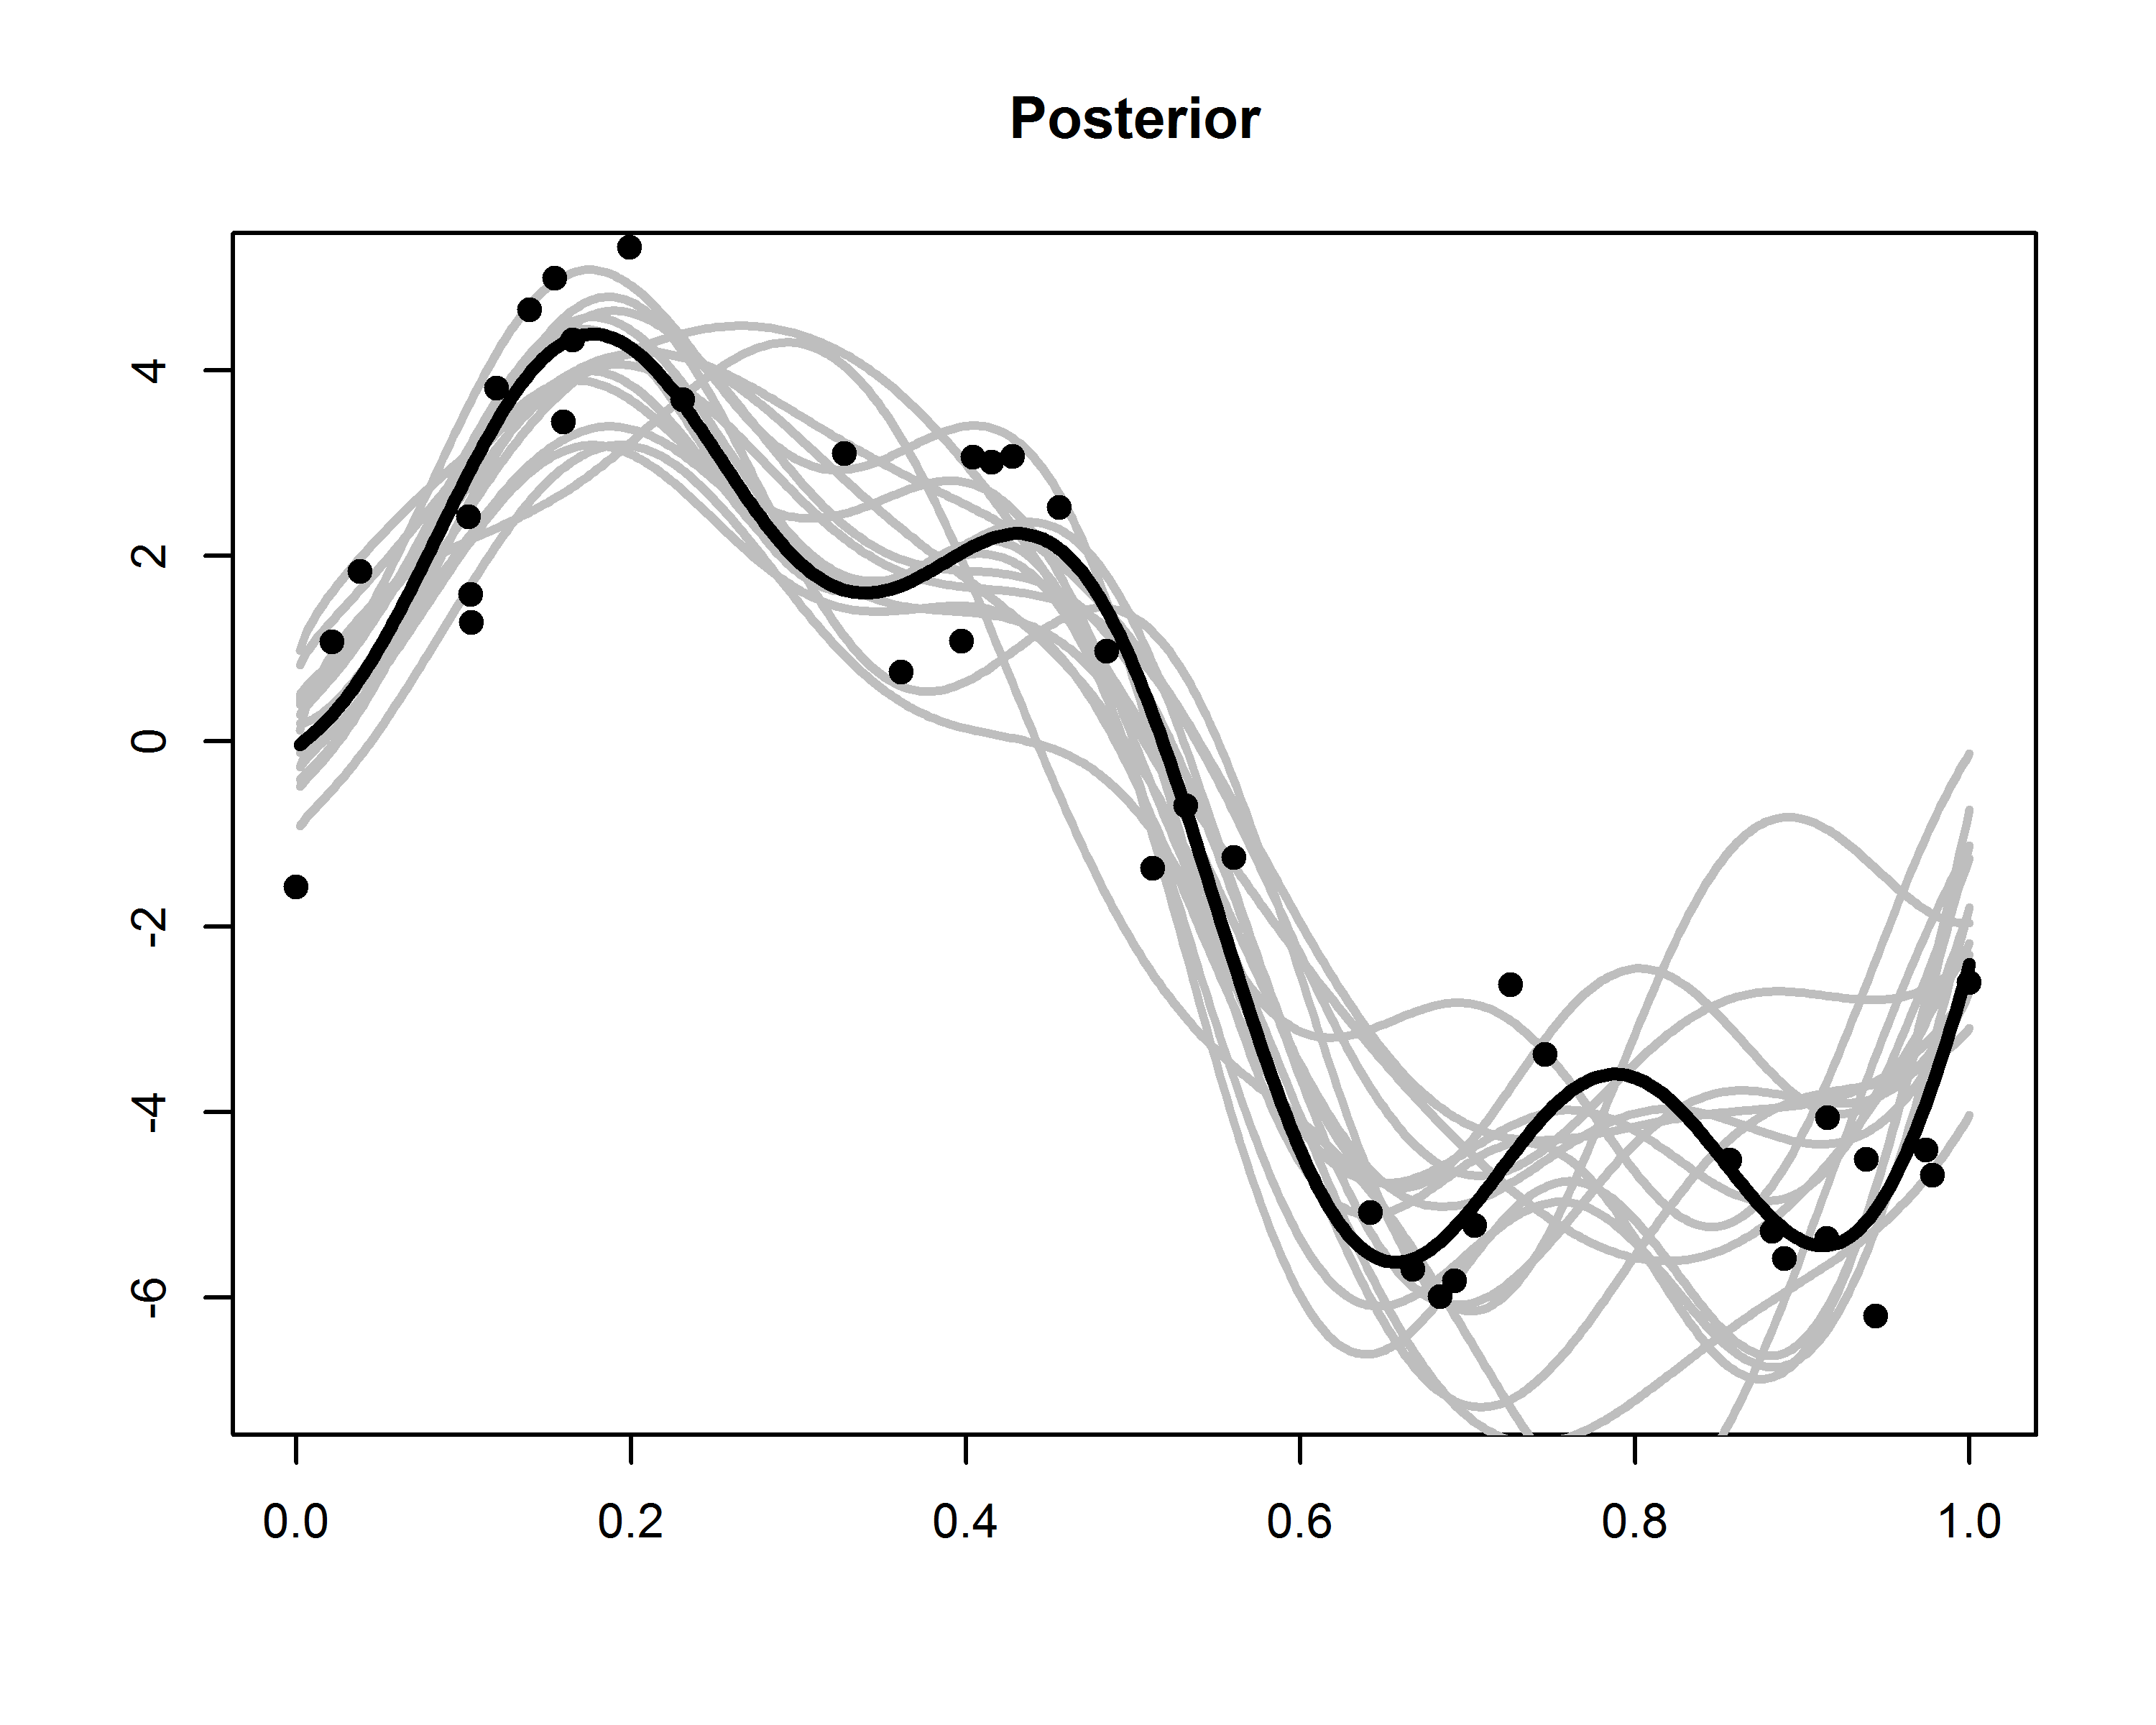
\includegraphics[width = 4in]{figures_julyan/Botond/Posterior.png}\vspace{-0.3cm}\\
}




\begin{frame}{Parametric versus nonparametric}
Complexity of the model $\{P_{\theta}:\, \theta\in\Theta\}$.\\
\vspace{-0.2cm}
\center{
\begin{tabular}{p{15mm}  p{42mm}  p{42mm}}
\toprule
Models&  \textbf{Parametric} & \textbf{Nonparametric}\\
\midrule
Dimension&  \textcolor{red}{Finite} dimensional $\Theta$ & \textcolor{red}{Infinite} dimensional $\Theta$ \\
&&\\
Pros&  \textcolor{red}{Easier} to handle and make interpretations of the results  & \textcolor{red}{Less} chance for \textcolor{red}{misspecifications } \\
& Computationally \textcolor{red}{faster } & More \textcolor{red}{flexible } \\
&&\\
Cons&  Without strong belief in the particular structure of the model \textcolor{red}{not reliable } &
\textcolor{red}{Computationally} and analytically \textcolor{red}{challenging }\\
&&\\
Examples&  \textcolor{red}{Poisson} (number of car crashes, typos in a book)  & Density, regression \textcolor{red}{function} estimation \\
& \textcolor{red}{Normal} distribution (grades of students, height, weight, footsize of people) &
\textcolor{red}{Clustering} (unknown cluster size and number)\\
\bottomrule
\end{tabular}
}
\end{frame}



%%%%%%%%%%%%%%%%%%%%%%%%%%%%%%%%%%%%%%%%%%%%%%%%%%%%%%%%%%%%%%%%%%%%%%%%%%%%%%%%%%%%%%%%%%%%%%%%%%%%%%

\frame{\frametitle{Noisy picture}
\center{

\includegraphics[width = 3.8in]{figures_julyan/Botond/Baby-Seal-Noisy3.jpg}
}}
\frame{\frametitle{Parametric}
\center{

\includegraphics[width = 3.8in]{figures_julyan/Botond/Baby-Seal-LowRes2.jpg}
}}
\frame{\frametitle{Nonparametric}
\center{
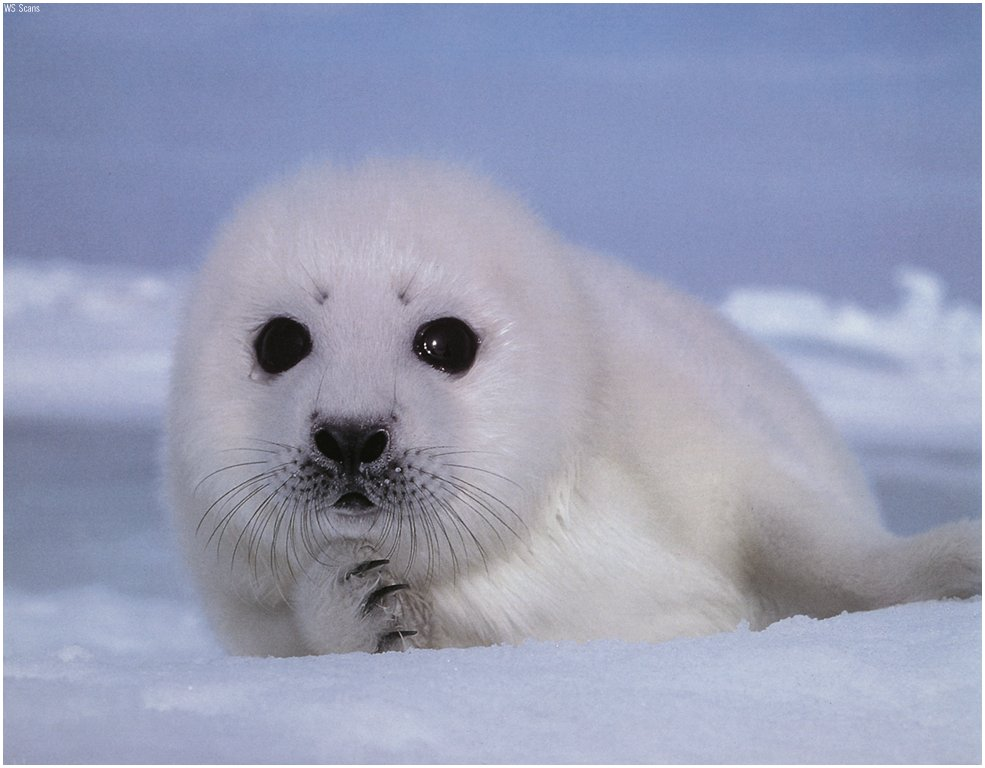
\includegraphics[width = 3.8in]{figures_julyan/Botond/Cute-Baby-Seal.jpg}
}}





\begin{frame}{Bayesian nonparametric priors}
\begin{block}{Two main categories of priors depending on parameter spaces}\medskip
\begin{columns}
\column{.4\textwidth}
%\begin{itemize}
%\item 
\visible<2->{\textcolor<2>{red2}{Spaces of functions\\\textit{random functions}}
\begin{itemize}
\item Continuous stochastic processes\\
e.g. Gaussian processes
\item Random basis expansions
\item Random densities (expon.)
%\end{itemize}
\end{itemize}}
\column{.6\textwidth}
%\begin{itemize}
%\item 
\visible<3->{\textcolor<3>{red2}{Spaces of probability measures\\\textit{random probability measures} (RPM)}
\begin{itemize}%[<+->]
\item \textcolor<4>{red2}{Often discrete proba. measures\\
Cornerstone: Dirichlet process}\\
We'll see others: Pitman--Yor, Normalized generalized gamma process, Normalized stable process, Gibbs-type processes, Normalized random measures, etc}
\end{itemize}
%\end{itemize}
\end{columns}
\end{block}
\begin{center}
\only<2>{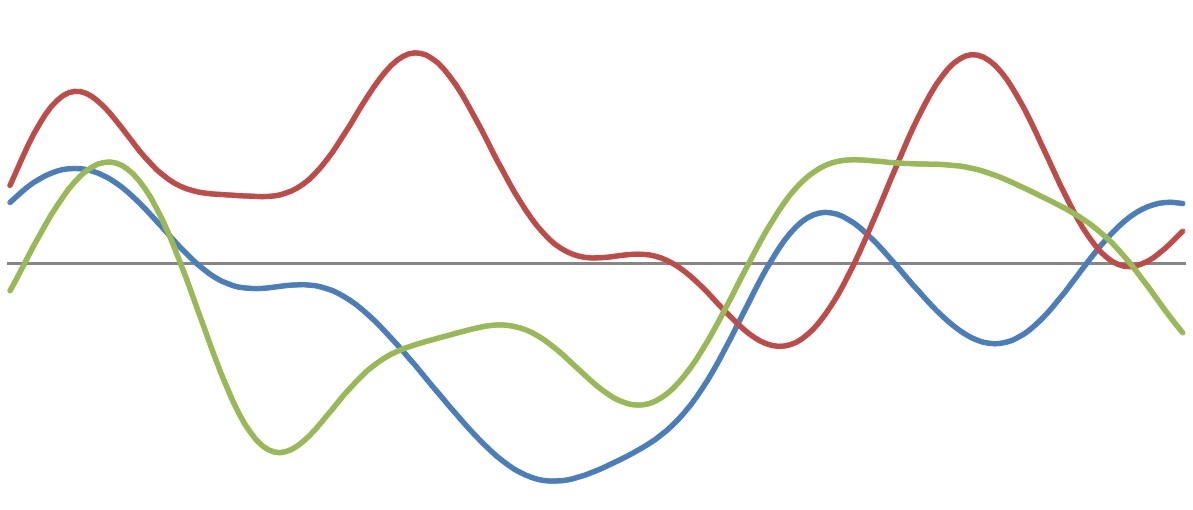
\includegraphics[width=.7\textwidth]{figures_julyan/introRPM/GPsamples}\\
\flushright[Wikipedia]}
\visible<3->{
\begin{center}
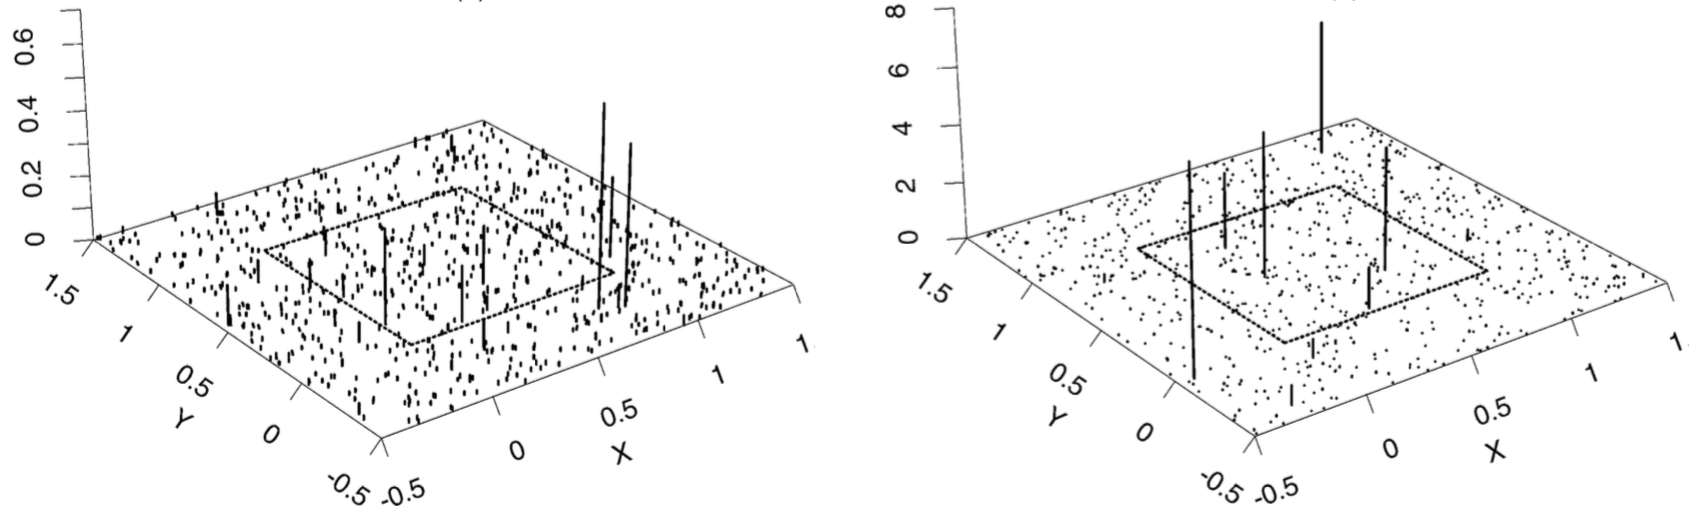
\includegraphics[width=\textwidth]{figures_julyan/introRPM/brix_draws}\\
\flushright %\textcolor{blue}
\citep{brix1999generalized}
\end{center}
}
%\visible<>{\includegraphics[width=\textwidth]{•}}
\end{center}
\end{frame}


%\section{Gaussian processes}


%%%%%%%%%%%%%%%%%%%%%%
\subsection{Introduction}
%%%%%%%%%%%%%%%%%%%%%%

\begin{frame}{What comes to $your$ mind when you hear ``Gaussian processes''?}
\end{frame}

\begin{frame}{Gaussian processes}
\begin{center}
	\only<1>{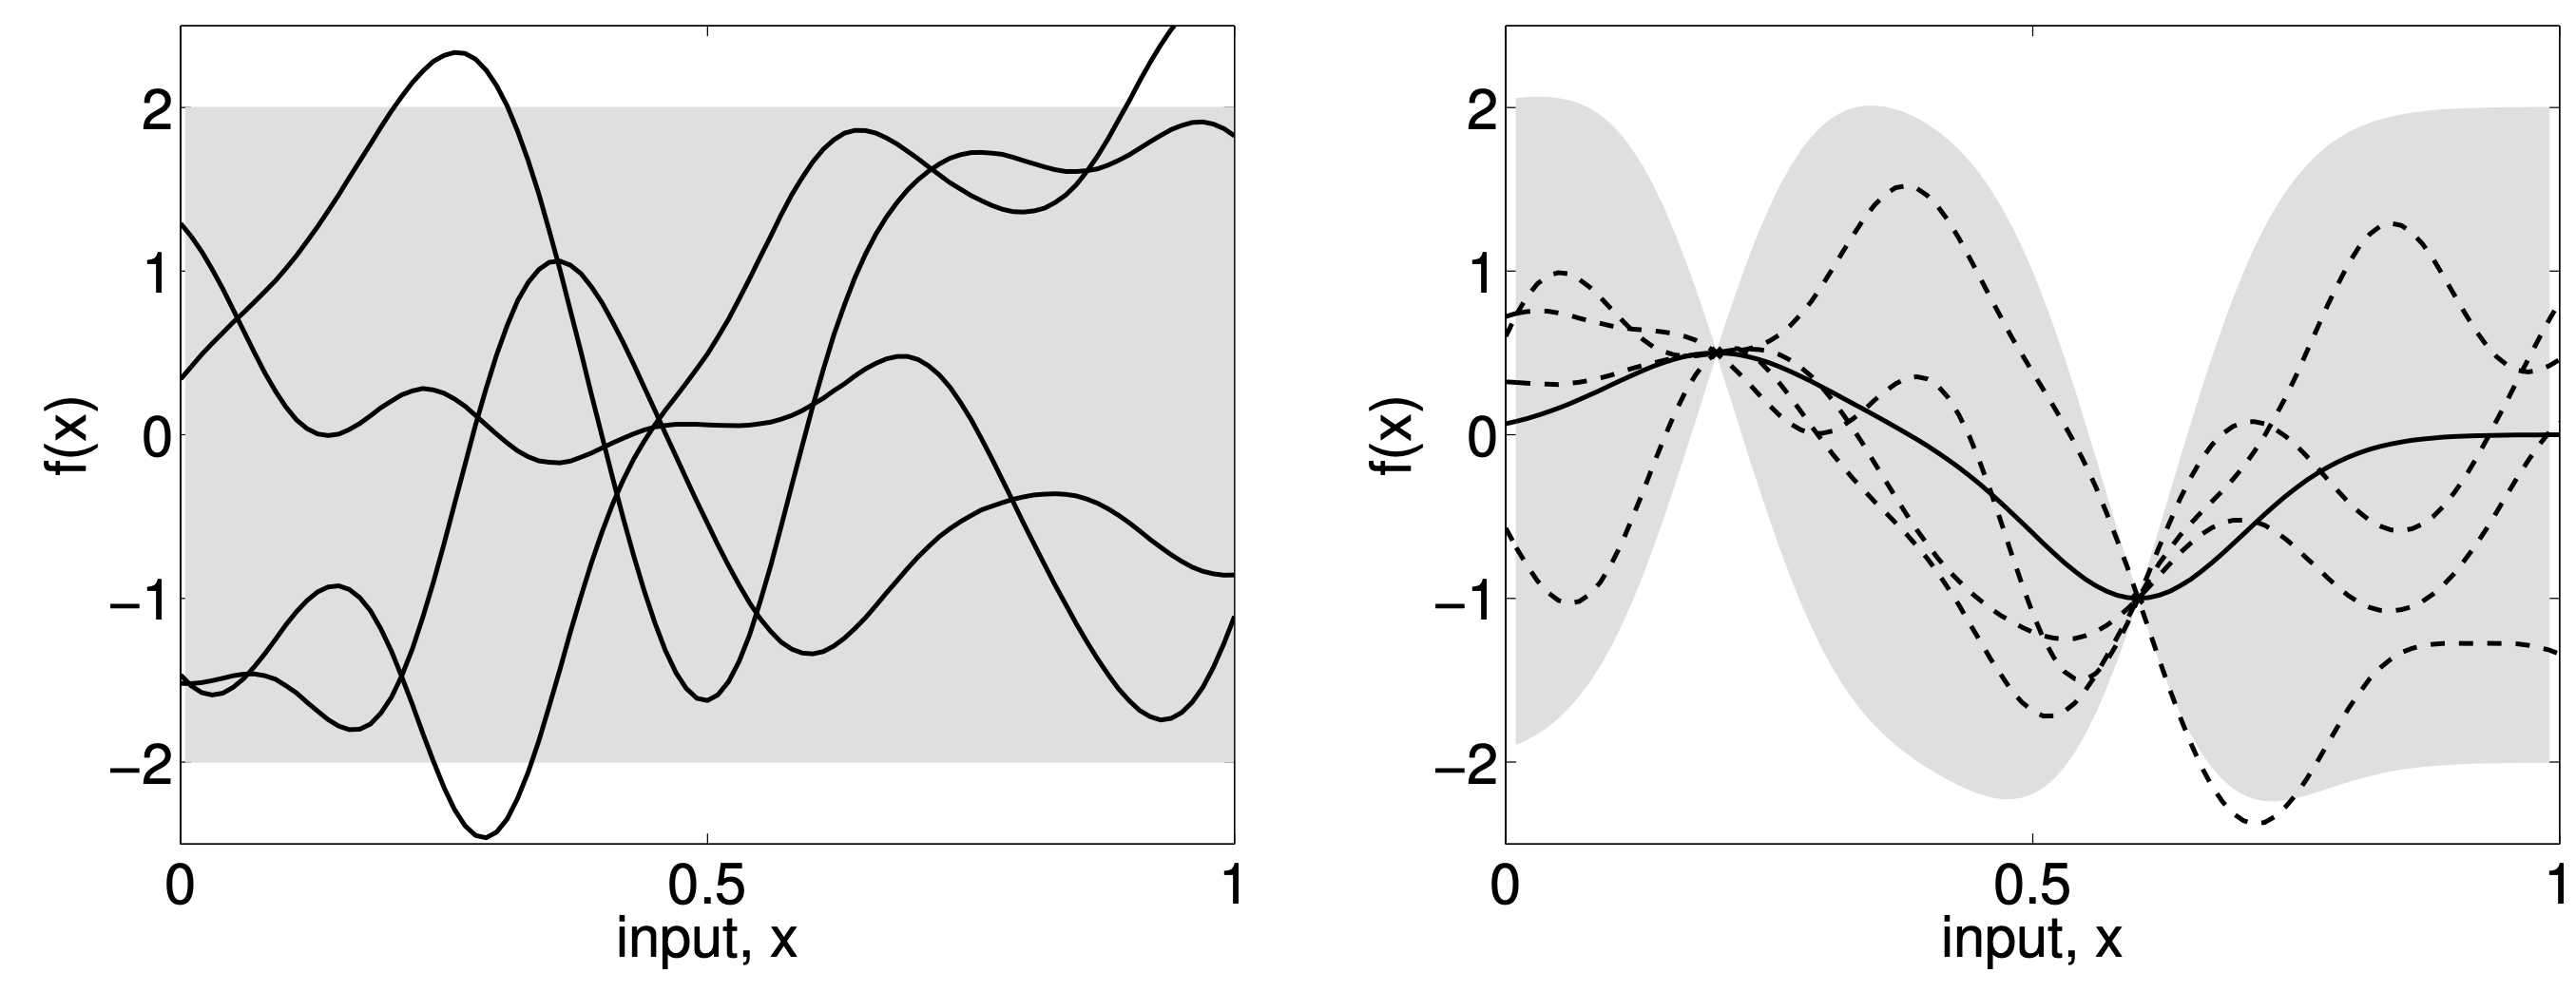
\includegraphics[height=.45\textheight]{figures_julyan/gp/gprw1}}
	\only<2>{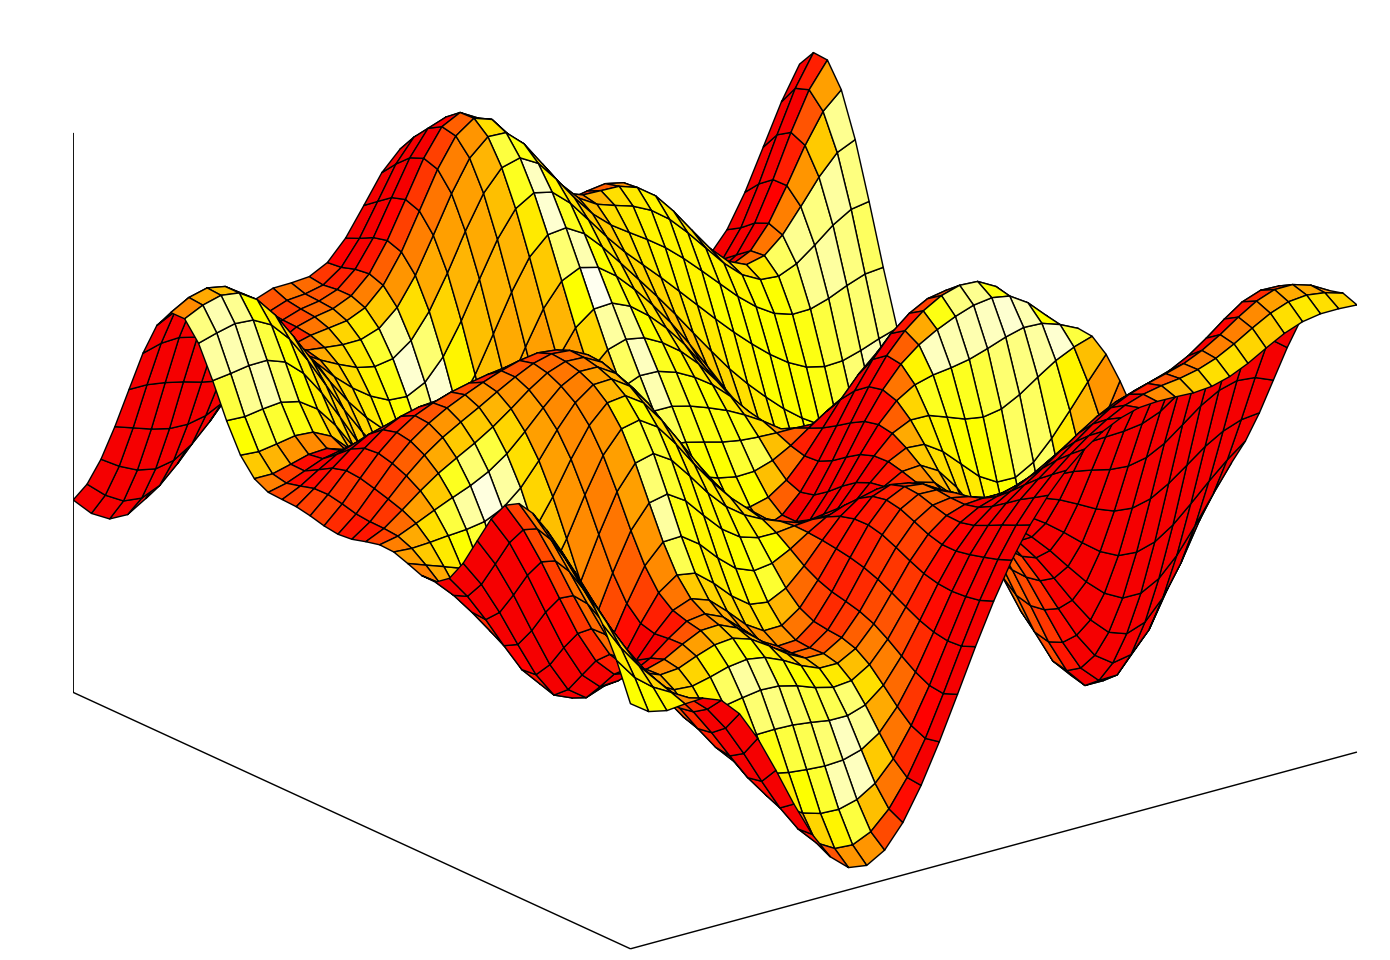
\includegraphics[height=.6\textheight]{figures_julyan/gp/gprw2}}
\end{center}
\hfill From \citet{Rasmussen:2006aa}
\end{frame}

\begin{frame}{Gaussian processes}
%\textcolor{gray}{What this chapter is about:}
%\begin{itemize}
%	\item How to use GPs in Bayesian inference
%	\item RKHS
%\end{itemize}\pause
%\textcolor{gray}{What this chapter is not about:}
%\begin{itemize}
%	\item Relationship with regularization theory, splines, support vector machines
%	\item PAC-Bayes analysis
%	\item Approximation methods: GP prediction methods is intractable for large sample $n$ datasets with complexity $\mathcal{O}(n^3)$ due to inversion of $n\times n$ matrix
%\end{itemize}\pause
\textcolor{gray}{Links with other chapters:}
\begin{itemize}
	\item GPs are used are \alert{BNP priors} on curves
	\item As such, the properties of the induced posterior are studied in the section on  \alert{asymptotics}
	\item Wide limit in  \alert{Bayesian neural networks}
	\item  \alert{SGD} with constant learning rate
	\item GPs are the nonparametric counterpart of the \alert{multivariate Gaussian distribution}, just like the \alert{Dirichlet process} is the nonparametric counterpart of the \alert{Dirichlet distribution}
\end{itemize}
\end{frame}


\begin{frame}{Gaussian process, Dirichlet process, and their parametric counterparts}
	\begin{center}
		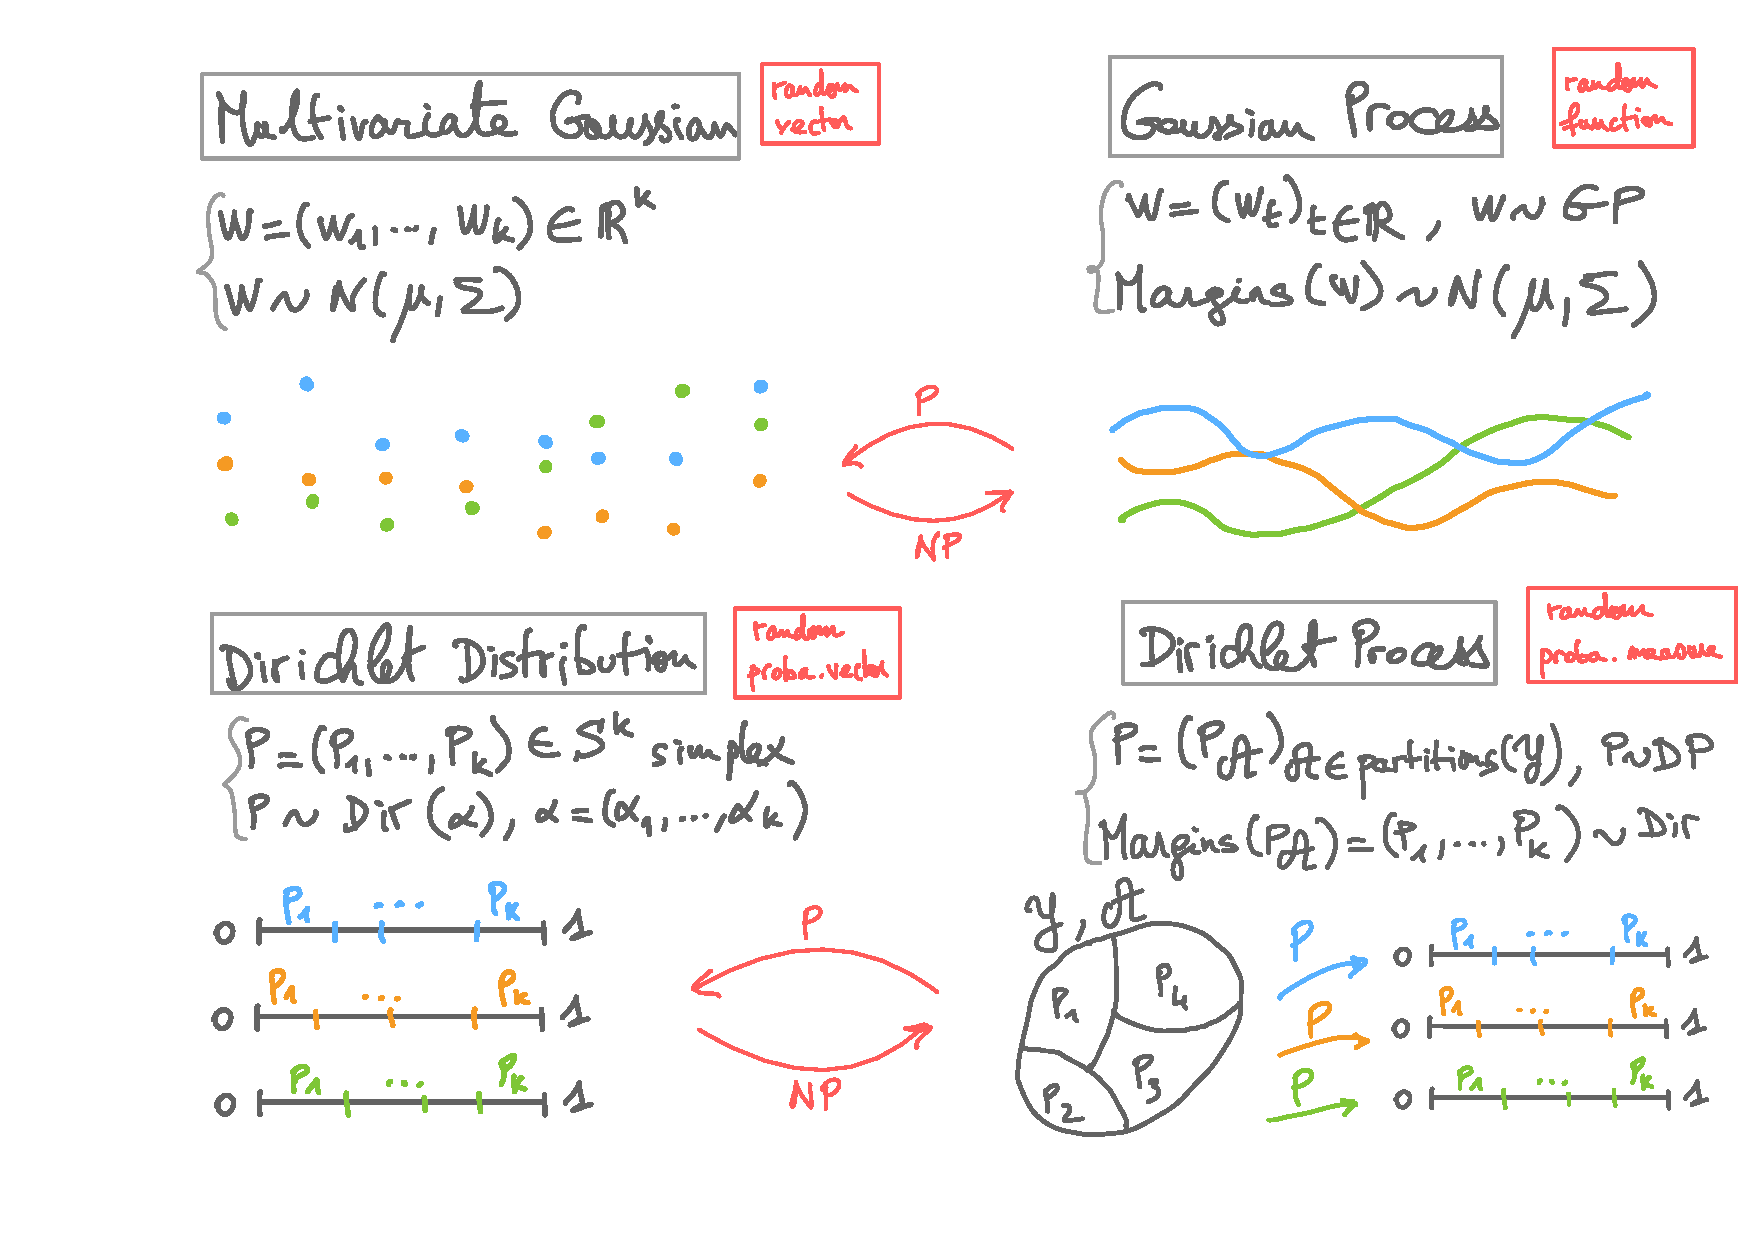
\includegraphics[width=\textwidth]{figures_julyan/gp/gp-and-dp.pdf}
	\end{center}
\end{frame}



\begin{frame}{References}
\begin{itemize}
	\item \alert{Main reference on GPs}: \fullcite{Rasmussen:2006aa}
	\item \alert{GPs in Bayesian inference}: Chapter 11 of \fullcite{ghosal2017fundamentals}
	\item \alert{Chapter 18} on Gaussian processes of \fullcite{murphy2023probabilisticMLadvanced}
\end{itemize}
\end{frame}




\begin{frame}{Supervized learning}

Two common approaches to \alert{supervized learning}:
\begin{itemize}
	\item restrict the class of functions considered, for example only linear functions of the input
	\item give a prior probability to every possible function, where higher probabilities are given to functions that we consider to be more likely
\end{itemize}

\end{frame}



\begin{frame}{Gaussian processes}
\begin{block}{Definition \citep{Rasmussen:2006aa}}
	A \alert{Gaussian process} is a collection of random variables, any finite number of which have a joint Gaussian distribution.
\end{block}

\pause

\begin{block}{Definition \citep{ghosal2017fundamentals}}
	A \alert{Gaussian process} is a stochastic process $W =(W_t: t \in T)$ indexed by an arbitrary set $T$ such that the vector $(W_{t_1},\ldots,W_{t_k})$ possesses a multivariate
normal distribution, for every $t_i\in T$ and $k\in \mathbb{N}$. A Gaussian process $W$ indexed by $\mathbb{R}^d$ is called:
\begin{itemize}
	\item  \alert{self-similar} of index $\alpha$ if $(W_{\sigma t}:t \in \mathbb{R}^d)$ is distributed like $(\sigma^\alpha W_{t}:t \in \mathbb{R}^d)$, for every $\sigma  > 0$, and 
	\item \alert{stationary} if $(W_{t+h}:t \in \mathbb{R}^d)$  has the same distribution of $(W_{t}:t \in \mathbb{R}^d)$, for every $h\in \mathbb{R}^d$.
\end{itemize}
\end{block}

\end{frame}



\begin{frame}{Mean function and covariance kernel}

Vectors $(W_{t_1},\ldots,W_{t_k})$ are called \alert{marginals}, and their distributions \alert{marginal distributions} or \alert{finite-dimensional distributions}

\pause


\begin{block}{Mean function and covariance kernel}
Finite-dimensional distributions are determined by the \alert{mean function} and \alert{covariance kernel}, defined by
$$\mu(t) = \E (W_t), \quad 
K(s, t) = \text{Cov}(W_s, W_t), \quad s, t \in  T.$$
\end{block}
\end{frame}



\begin{frame}{Scaling}

\begin{alertblock}{Scaling}
If $W =(W_t: t \in \mathbb{R}^d)$ is a Gaussian process  with covariance kernel $K$, then the process $(W_{\sigma t}: t \in \mathbb{R}^d)$ is another Gaussian process, with covariance kernel $K(\sigma s, \sigma t)$, for any $\sigma  > 0$. A scaling factor $\sigma  > 1$ shrinks the sample paths, whereas a factor $\sigma  < 1$ stretches them.
\end{alertblock}

\pause

\begin{center}
	\only<2>{
	$\sigma  > 1$ \hspace{4.5cm} $\sigma  < 1$ 
	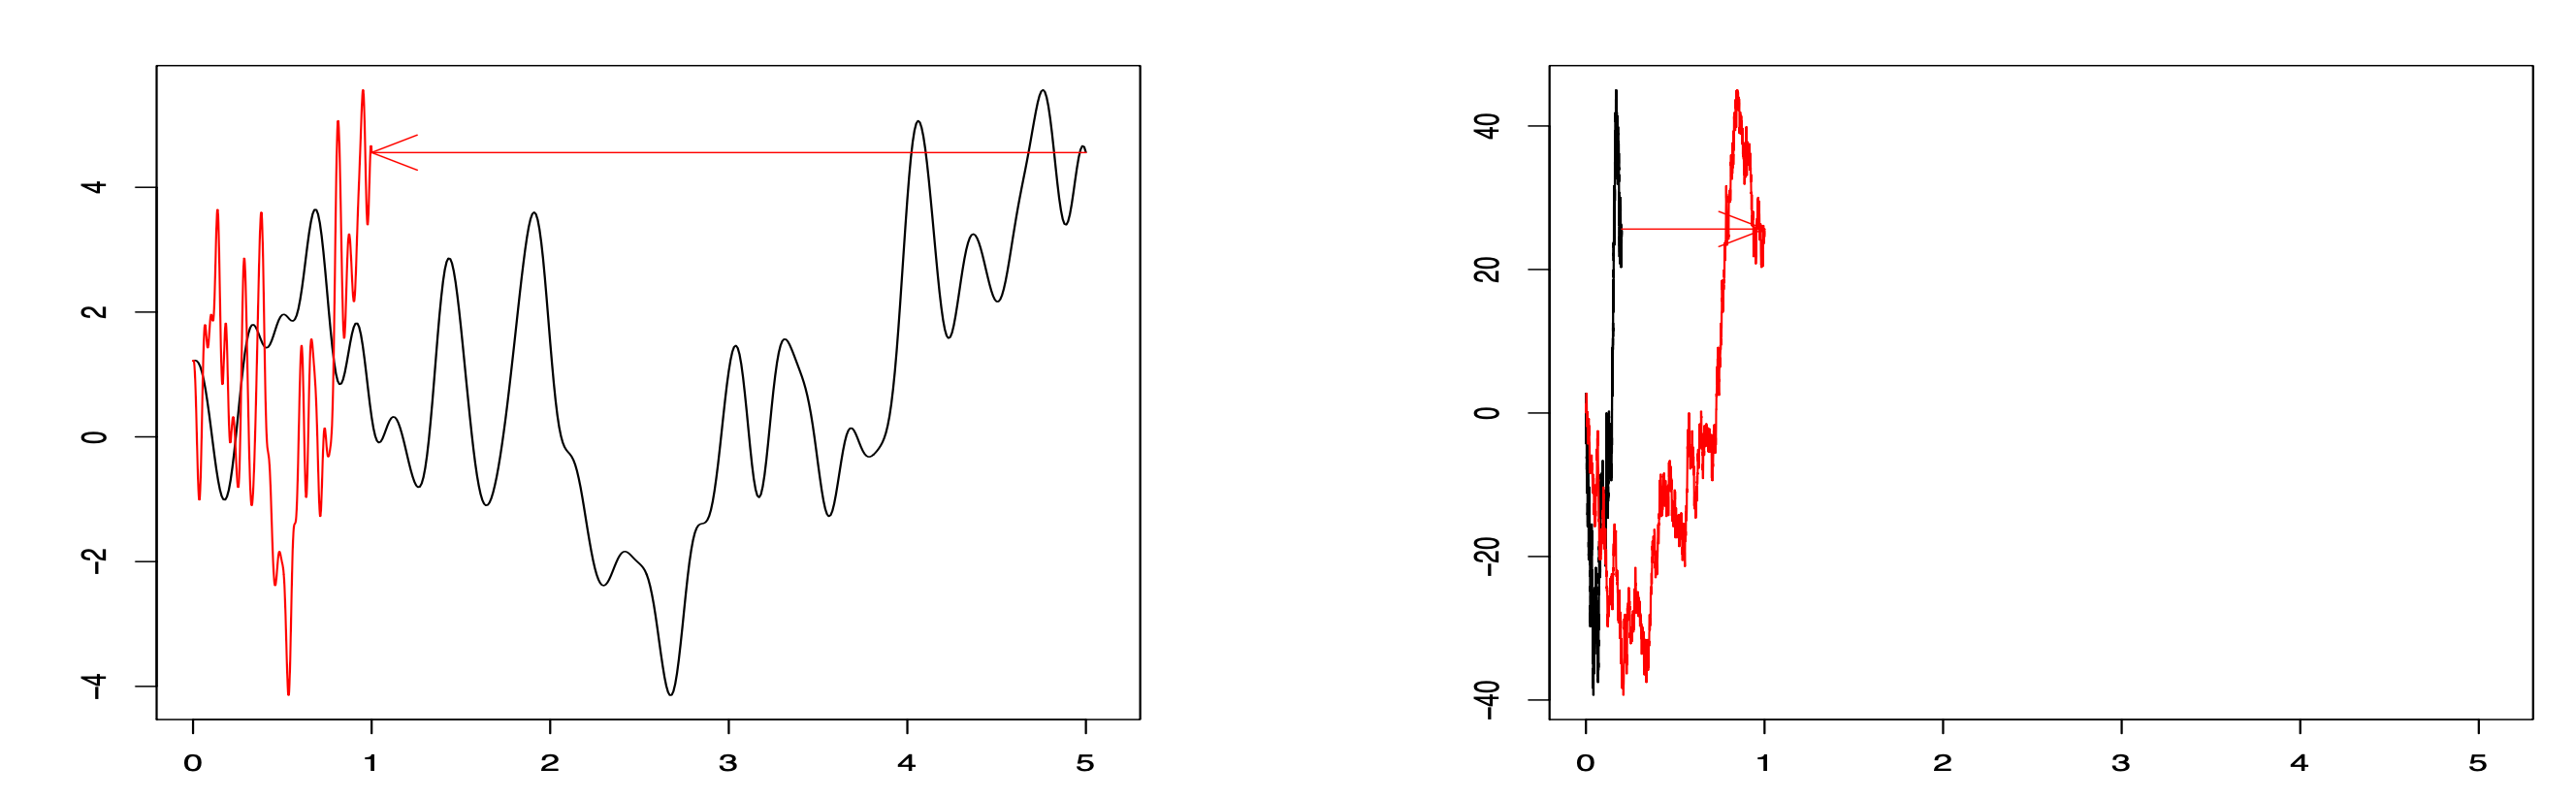
\includegraphics[height=.35\textheight]{figures_julyan/gp/scaling}
	}
\end{center}
\hfill From \citet{ghosal2017fundamentals}


\end{frame}


\subsection{Examples}


\begin{frame}{Examples}
\begin{exampleblock}{Random series}
	If $Z_1,\ldots,Z_m\simiid \mathcal{N}(0,1)$ and $a_1,\ldots,a_m$ are [deterministic] functions, then the \textit{Random series} $W_t = \sum_{i=1}^m a_i(t)Z_i$ defines a Gaussian process with:\bigskip
	
		\indent $\mu(t)=$\bigskip
		
		\indent $K(s, t)=$
%	\begin{align*}
%		\mu(t) & = \\
%		K(s, t) & = 
%	\end{align*}
\end{exampleblock}

\end{frame}


\begin{frame}{Examples}

\begin{exampleblock}{Brownian motion (or Wiener process)}
	The \textit{Brownian motion} is the zero-mean Gaussian process, say on $[0,\infty)$, with continuous sample paths and covariance function $K(s,t)=\min(s,t)$.
\end{exampleblock}

\pause


\begin{alertblock}{Brownian motion properties}
	Let $B_t$ be a Brownian motion, then $\forall s< t$:
	\begin{itemize}
		\item \alert{Stationarity}:  $B_t-B_s\sim \mathcal{N}(0,t-s)$
		\item \alert{Independent increments}:  $B_t-B_s \perp\!\!\!\!\perp (B_u, u\leq s)$
	\end{itemize}
	Thus it is a L\'evy process.
	\begin{itemize}
		\item \alert{Self-similar} of index $1/2$.
	\end{itemize}
\end{alertblock}

\end{frame}


\begin{frame}{Examples}

\begin{exampleblock}{Ornstein--Uhlenbeck}
	The standard \textit{Ornstein--Uhlenbeck process} with parameter $\theta>0$ is a mean-zero, stationary GP with time set $T = [0, \infty)$, continuous sample paths, and covariance function
		$$K(s,t) = (2\theta)^{-1}\exp\left(-\theta|t-s|\right).$$
\end{exampleblock}

\pause

\begin{alertblock}{Properties of Ornstein--Uhlenbeck process}
	The standard Ornstein--Uhlenbeck process with parameter $\theta>0$ can be constructed from a Brownian motion $B$ through the relation 	
	$$W_t = (2\theta)^{-1/2}\exp\left(-\theta t\right)B_{e^{2\theta t}}.$$
\end{alertblock}

\pause

Relationship between [fixed learning rate] \alert{stochastic gradient descent} (SGD) and \alert{Markov chain Monte Carlo} (MCMC) through the Ornstein--Uhlenbeck process: see \citet{mandt2017stochastic}.


\end{frame}


\begin{frame}{Examples}

	
\begin{exampleblock}{Square exponential}
	GP with covariance function (a.k.a. radial basis function kernel)
	$$K(s,t) = \exp\left(-\frac{\Vert t-s\Vert^2}{2\ell^2}\right).$$
	Parameter $\ell$ is called the \textit{characteristic length-scale}.
\end{exampleblock}


\begin{exampleblock}{Fractional Brownian motion}
	The \textit{fractional Brownian motion} (fBm) with \textit{Hurst parameter} $\alpha\in  (0, 1)$ is the mean zero Gaussian process $ W = (W_t : t \in  [0, 1])$ with continuous sample paths and covariance function
	$$K(s,t) = \frac{1}{2}\left(s^{2\alpha}+t^{2\alpha}-|t-s|^{2\alpha}\right).$$
	\begin{itemize}
		\item $\alpha=1/2$ yields the standard Brownian motion.
	\end{itemize}
\end{exampleblock}
	
\end{frame}


\begin{frame}{Practical}
\begin{alertblock}{Practical}
	\ComputerMouse\,\, Try practical on Gaussian process sampling,  \alert{gaussian-process-sampling.ipynb}.
\end{alertblock}
\end{frame}

\subsection{Gaussian process regression}


\begin{frame}{Conditional distributions of a multivariate Gaussian}
Let an $N$-dimensional Gaussian vector $\mathbf {x}$  be partitioned as:\\  
$\mathbf {x}={\begin{bmatrix}\mathbf {x} _{1}\\\mathbf {x} _{2}\end{bmatrix}}$ with sizes $q$ and $N-q$, and accordingly ${\boldsymbol {\mu }}$ and ${\boldsymbol \Sigma}$ are partitioned as
${\boldsymbol {\mu }}={\begin{bmatrix}{\boldsymbol {\mu }}_{1}\\{\boldsymbol {\mu }}_{2}\end{bmatrix}}$ with sizes $q$ and $N-q$ and 
$${\displaystyle {\boldsymbol {\Sigma }}={\begin{bmatrix}{\boldsymbol {\Sigma }}_{11}&{\boldsymbol {\Sigma }}_{12}\\{\boldsymbol {\Sigma }}_{21}&{\boldsymbol {\Sigma }}_{22}\end{bmatrix}}{\text{ with sizes }}{\begin{bmatrix}q\times q&q\times (N-q)\\(N-q)\times q&(N-q)\times (N-q)\end{bmatrix}}}.$$
Then 
\begin{itemize}
	\item the \alert{conditional distribution} of $ \mathbf x_1$, conditioned on $\mathbf x_2 = a$, is multivariate normal $\mathcal{N}_q( \bar{ \boldsymbol {\mu} }, \bar{ \boldsymbol {\Sigma} })$ where
${ {\bar {\boldsymbol {\mu }}}={\boldsymbol {\mu }}_{1}+{\boldsymbol {\Sigma }}_{12}{\boldsymbol {\Sigma }}_{22}^{-1}\left(\mathbf {a} -{\boldsymbol {\mu }}_{2}\right)}$
and 
${ {\bar {\boldsymbol {\Sigma }}}={\boldsymbol {\Sigma }}_{11}-{\boldsymbol {\Sigma }}_{12}{\boldsymbol {\Sigma }}_{22}^{-1}{\boldsymbol {\Sigma }}_{21}}$;
	\item the \alert{marginal (unconditional) distribution} of $ \mathbf x_1$ is multivariate normal $\mathcal{N}_q( \boldsymbol {\mu}_1, \boldsymbol {\Sigma }_{11})$.
\end{itemize}

\end{frame}


\begin{frame}{Gaussian process regression without noise}
	Let a regression function modeled by a Gaussian process as follows:
%
\begin{equation*}
       \mathbf{f} \, \lvert\, \mathbf{X} \sim GP(\mathbf{f} \, \lvert\, \boldsymbol\mu, \mathbf{K}), 	
\end{equation*}
where $\mathbf{X} = [\mathbf{x}_1, \ldots, \mathbf{x}_n ]$ represents the observed data points, $\mathbf{f} = \left[ f(\mathbf{x}_1), \ldots, f(\mathbf{x}_n) \right]$ the function values, $\boldsymbol\mu = \left[ m(\mathbf{x}_1), \ldots, m(\mathbf{x}_n) \right]$ the mean function, and $K_{ij} = k(\mathbf{x}_i,\mathbf{x}_j)$ the kernel function. Assume $\boldsymbol\mu=0$. We want to predict $\mathbf{f}(\mathbf{X}_*)$ at new points $\mathbf{X}_*$. The joint distribution of $\mathbf{f}$ and $\mathbf{f}_*$ is expressed as:
%
    \begin{align}
       \begin{bmatrix}\mathbf{f} \\ \mathbf{f}_*\end{bmatrix} \sim \mathcal{N}\left(\mathbf{0}, \begin{bmatrix}\mathbf{K} & \mathbf{K}_* \\ \mathbf{K}_*^\mathsf{T} & \mathbf{K}_{**}\end{bmatrix}\right), \nonumber
    \end{align}
%
where $\mathbf{K}=K(\mathbf{X}, \mathbf{X})$, $\mathbf{K}_* = K(\mathbf{X}, \mathbf{X}_*)$ and $\mathbf{K}_{**}=K(\mathbf{X}_*, \mathbf{X}_*)$. The conditional distribution of interest is:
\begin{align}
       \mathbf{f}_* \, \vert \, \mathbf{f}, \mathbf{X}, \mathbf{X}_* \sim \mathcal{N} \left(\mathbf{K}_*^\mathsf{T} \, \mathbf{K}^{-1} \, \mathbf{f}, \: \mathbf{K}_{**} - \mathbf{K}_*^\mathsf{T} \, \mathbf{K}^{-1} \, \mathbf{K}_* \right). \nonumber
    \end{align}
\end{frame}


\begin{frame}{Gaussian process regression with noise}
Oftentimes, we only have access to noisy versions of the true function, $y = f(x) + \epsilon$, where $\epsilon$ represents additive i.i.d. Gaussian noise with variance $\alert{\sigma^2}$. Then $\text{cov}(y) = \mathbf{K} + \alert{\sigma^2} \mathbf{I}$. The joint distribution of the observed values and the function values at new testing points is:
%
    \begin{align}
       \begin{pmatrix}\mathbf{y} \\ \mathbf{f}_*\end{pmatrix} \sim\mathcal{N}\left(\mathbf{0}, \begin{bmatrix}\mathbf{K} + \alert{\sigma^2} \mathbf{I} & \mathbf{K}_* \\ \mathbf{K}_*^\mathsf{T} & \mathbf{K}_{**}\end{bmatrix}\right) \ . \nonumber
    \end{align}
%
Using the conditional distribution, we now get:
%
    \begin{align}
       \mathbf{{f}_*} \, \vert \, \mathbf{X}, \mathbf{y}, \mathbf{X}_* \sim \mathcal{N} \left(\mathbf{K}_*^\mathsf{T} [\mathbf{K} + \alert{\sigma^2} \mathbf{I}]^{-1} \mathbf{y}, \mathbf{K}_{**} - \mathbf{K}_*^\mathsf{T} [\mathbf{K} + \alert{\sigma^2} \mathbf{I}]^{-1} \mathbf{K}_*\right). \nonumber
    \end{align}	
\end{frame}

\begin{frame}{Practical}
\begin{alertblock}{Practical}
	\ComputerMouse\,\, Try practical on Gaussian process regression,  \alert{gaussian-process-regression.ipynb}.
\end{alertblock}
\end{frame}


%
%\begin{frame}{Kriging}
%
%\begin{exampleblock}{Kriging}
%	For a given Gaussian process $W = (W_t : t \in T)$ and fixed, distinct points $t_1,\ldots,t_m \in T$, the conditional expectations $W_t^\star  = \E [ W_t|W_{t_1},\ldots,W_{t_m}]$ define another Gaussian process.
%\end{exampleblock}
%
%\pause 
%
%\begin{block}{Exercise}
%	Find the covariance function of $W_t^\star$, say $K^\star(t,s)$, as a function of $(t_1,\ldots,t_m)$.
%\end{block}
%
%\pause 
%
%\begin{alertblock}{Properties of Kriging}
%	\begin{itemize}
%		\item If $W$ has continuous sample paths, then so does $W^\star$. 
%		\item In that case the process $W^\star$ converges to $W$ when $m \to \infty$  and the interpolating points $(t_1,\ldots,t_m)$ grow dense in $T$.
%	\end{itemize}
%\end{alertblock}
%\end{frame}

\subsection{Reproducing kernel Hilbert space}

\begin{frame}{Reproducing kernel Hilbert space}
	To every Gaussian process corresponds a Hilbert space, determined by its covariance kernel. This space determines the support and shape of the process, and therefore is crucial for the properties of the Gaussian process as a prior. 

\pause

Let's break down what each part means:

\alert{Reproducing Kernel}: This refers to a mathematical function that takes in two inputs and calculates a measure of similarity or distance between them. It's called \alert{reproducing} because it has a special property related to the inner product (a mathematical operation) that allows it to reproduce functions.

\alert{Hilbert Space}: This is a mathematical concept from functional analysis, which is basically a fancy way of saying a space where functions live. A Hilbert space is a mathematical structure that generalizes the notion of Euclidean space to infinite-dimensional spaces (formal def: inner product space that is complete wrt the distance function induced by the inner product).

%\pause
%
%\begin{block}{Definition}
%	A \textit{Hilbert space} is an inner product space that is complete wrt the distance function induced by the inner product.
%\end{block}
\end{frame}


\begin{frame}{Reproducing kernel Hilbert space}
For a Gaussian process $W = (W_t : t \in T)$, let $\overline{\text{lin}}(W)$ be the closure of the set of all linear combinations $\sum_I \alpha_i W_{t_i}$ in the $L_2$-space of square-integrable variables. The space $\overline{\text{lin}}(W)$ is a Hilbert space.

\pause

\begin{block}{Definition} 
The \textit{reproducing kernel Hilbert space} (RKHS) of the mean-zero, Gaussian process $W = (W_t : t \in T )$ is the set $\mathbb{H}$ of all functions $z_H:T \to \mathbb{R}$ defined by $z_H(t) = \E(W_t H)$, for $H$ ranging over $\overline{\text{lin}}(W)$. The corresponding inner product is
	$$\langle z_{H_1},z_{H_2}\rangle_{\mathbb{H}} =  \E (H_1H_2).$$
\end{block}
\end{frame}


\begin{frame}[allowframebreaks]{Reproducing kernel Hilbert space}

\begin{alertblock}{Properties of RKHS}
	\begin{itemize}
		\item Correspondance $z_H \leftrightarrow H$ is an isometry (by def of inner product), so the definition is well-posed (the correspondence is one-to-one), and $H$ is indeed a Hilbert space.
		\item Function corresponding to $H=\sum_I \alpha_i W_{s_i}$ is \bigskip
			$z_H=$
		\item For any $s\in T$, function $K(s,\cdot)$ is in RKHS $\mathbb{H}$ associated with $H = W_s$.
	\end{itemize}
\end{alertblock}

\framebreak

\begin{alertblock}{Reproducing formula}
For a general function $z_H \in \mathbb{H}$ we have $$\langle z_H, K(s, \cdot)\rangle_{\mathbb{H}} = \E (H W_s) = z_H(s).$$
That is to say, for any function  $h \in \mathbb{H}$,
	$$h(t) = \langle h, K(t, \cdot)\rangle_{\mathbb{H}}.$$
\end{alertblock}

\end{frame}

\begin{frame}{Example of RKHS: Euclidean space}
Let's consider a simple \alert{Euclidean space}, such as  $\mathbb{R}$. In this case, the RKHS corresponds to a space of functions defined on this real line.

Consider a set of data points on the real line, represented by pairs \((x_i, y_i)\) where \(x_i\) are the input values and \(y_i\) are the corresponding output values.

Let's model this data with a function \(f(x)\). In an RKHS framework, we can express this function as a linear combination of \alert{basis functions} \(k(x, x_i)\), where \(k\) is a  \alert{kernel function} that measures the similarity between input points \(x\) and \(x_i\).

The RKHS then consists of all functions that can be expressed as:
%
\[f(x) = \sum_{i=1}^{n} \alpha_i k(x, x_i)\]
%
where \(\alpha_i\) are coefficients that determine the weighting of each basis function.

Common choices for the kernel function in this context might be the linear kernel \(k(x, x_i) = x \cdot x_i\), the polynomial kernel \(k(x, x_i) = (x \cdot x_i + c)^d\), or the Gaussian kernel \(k(x, x_i) = \exp(-\|x - x_i\|^2 / 2\sigma^2)\).

The RKHS provides a flexible framework for modeling functions in this space using different kernel functions, allowing us to capture various types of relationships between input and output data points.\end{frame}


\section{Discrete random probability measures}


\subsection{Introduction}


\begin{frame}{References}
\begin{itemize}
	\item \alert{One of the first textbooks on the Dirichlet process}: \fullcite{Ghosh2003}
	\item \alert{One that reads very well}: \fullcite{hjort2010bayesian}
	\item \alert{Chapter 14} on Discrete Random Structures of \fullcite{ghosal2017fundamentals}
\end{itemize}
\end{frame}


\subsection{Dirichlet process}

\begin{frame}{Dirichlet distribution}
	The \textit{Dirichlet distribution} on the simplex $\Delta_K$ is a probability distribution with parameter $\boldsymbol{\alpha} = (\alpha_1,\ldots,\alpha_K)$ with $\alpha_j>0$ and density function, for $\boldsymbol{x} = (x_1, \ldots, x_K)\in \Delta_K$,
\begin{displaymath}
f(\boldsymbol{x}; \boldsymbol{\alpha}) = \frac{1}{B(\alpha)}\prod_{i=1}^Kx_i^{\alpha_i - 1}.
\end{displaymath}
% where $(x_i)$ form a simplex. 

The Dirichlet distribution is conjugate for the multinomial distribution. 

\begin{center}
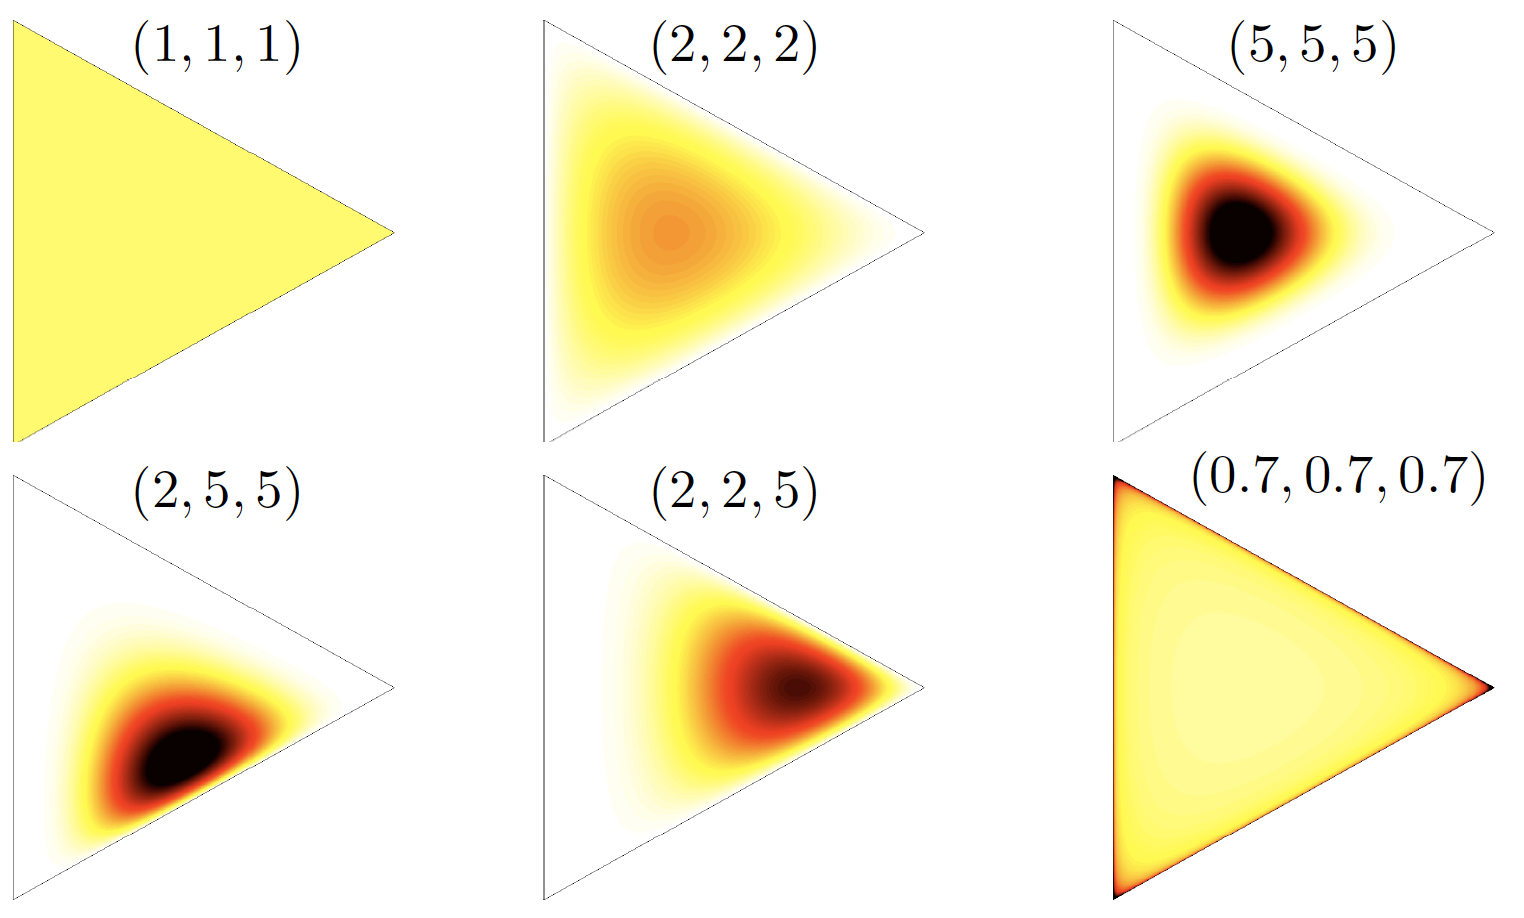
\includegraphics[width = .6\textwidth]{figures_julyan/intro_DP/dirichlet_distribution}
\end{center}
\hfill\textcolor{gray}{[Image by Y.W. Teh]}
\end{frame}


\begin{frame}{Dirichlet process}
A central Bayesian nonparametric prior \citep{ferguson1973bayesian}.\pause

\begin{block}{Definition (Dirichlet process)}
A \alert{Dirichlet process} on the space $\mathcal{Y}$ is a random process $ P $ such that there exist $ \alpha>0 $ (precision parameter) and $ P_0 $ (base/centering distribution) \pause such that for any finite partition $ \{A_1,\ldots,A_k\} $ of $\mathcal{Y}$, the random vector
$ (P(A_1),\ldots,P(A_k)) $ is Dirichlet distributed
\[ (P(A_1),\ldots,P(A_k))\sim \text{Dir}(\alpha P_0(A_1),\ldots,\alpha P_0(A_k)) \]
\textit{Notation}: $ P \sim \text{DP}(\alpha, P_0) $
\end{block}
\begin{center}
\visible<3->{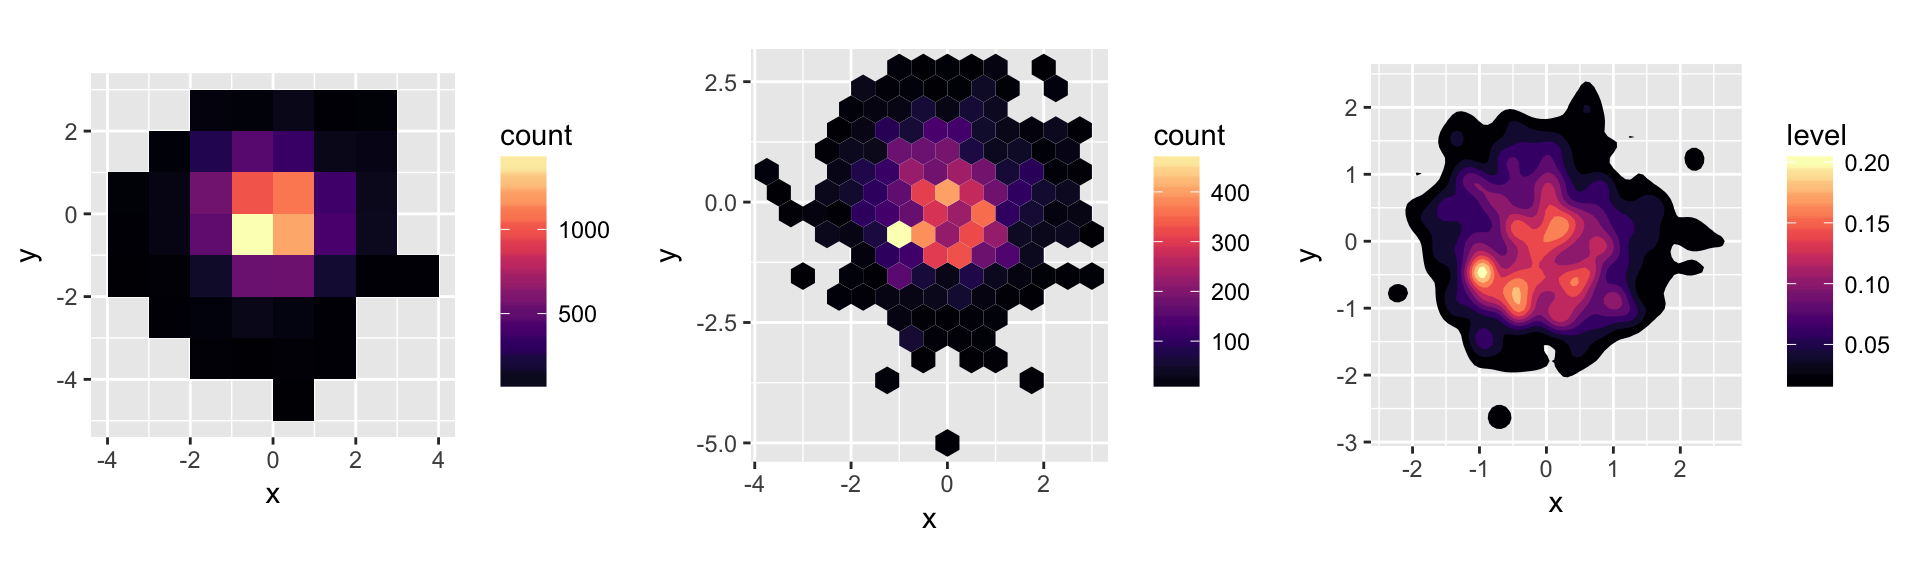
\includegraphics[width=\textwidth]{figures_julyan/intro_DP/DP_marginal}}
%\animategraphics[loop, width=\textwidth]{2}{figures_julyan/intro_DP/density_2D_}{1}{10} % pb ici: should specify pdf for images...
\end{center}
\end{frame}

\begin{frame}[allowframebreaks]{Moments of Dirichlet process}
	\begin{proposition}
Let $P\sim \text{DP}(\PrecisonParam, P_0)$ then for every measurable sets $A, B$ we have
\begin{align*}
    \E[ P(A)] &= P_0(A),\\
    \Var[P(A)] &= \frac{P_0(A)(1-P_0(A))}{1+\PrecisonParam},\\
    \Cov( P(A), P(B) )&=\frac{P_0(A \cap B) - P_0(A)P_0(B) }{1+\PrecisonParam}\label{Dir:Covariance}.
\end{align*}
\end{proposition}

% \begin{enumerate}
%     \item $\E( p(A)) = P_0(A)$,
%     \item ${\rm Var}(p(A)) = \frac{P_0(A)(1-P_0(A))}{1+\PrecisonParam}$,
%     \item $\Cov( p(A), p(B) )=\frac{P_0(A \cap B) - P_0(A)P_0(B) }{1+\PrecisonParam}$.
% \end{enumerate}
\framebreak

\textbf{Proof.}
We will make use of  $p(A)\sim \Beta(\alpha P_0(A), \alpha (1-P_0(A)))$. From this we obtain 
\begin{equation*}
    \E (p(A)) = \frac{\PrecisonParam P_0(A)}{\PrecisonParam( P_0(A) + 1 - P_0(A) )} = P_0(A)
\end{equation*}
and 
\begin{equation*}
    \Var(p(A))=\frac{\PrecisonParam^2 P_0(A)( 1-P_0(A) )}{\PrecisonParam^2 (\PrecisonParam + 1)}.
\end{equation*}
We derive the covariance term in two cases, firstly taking into consideration the one with $A\cap B = \emptyset$. In that case any space $\Omega$ may be decomposed into three sets: 
$$
\Omega = \{A, B, (A\cup B)^c\}.
$$
Using de Morgan's law the last can be written as $(A\cup B)^c = A^c\cap B^c =: C$. Therefore we may write a joint probability vector
\begin{equation*}
    \big( P(A), P(B), P(A^c\cap B^c) \big)\sim \Dir\big(\PrecisonParam P_0(A), \PrecisonParam P_0(B), \PrecisonParam P_0(C) \big)
\end{equation*}
and hence $\Cov(P(A), P(B)) = -P_0(A)P_0(B)/(1+\PrecisonParam) $. 
In the more general case one may decompose 
\begin{align*}
    A &= (A\cap B) \cup (A\cap B^c)\\
    B &= (B\cap A)\cup (B\cap A^c),
\end{align*}
so that 
\begin{equation*}
    \begin{split}
    \Cov (P(A), P(B)) &= \Cov (P(A\cap B) +P(A\cap B^c), P(B\cap A) + P(B\cap A^c) ) 
    % &=\Cov (P(A\cap B) , P(B\cap A)  ) + \Cov (P(A\cap B),  P(B\cap A^c) ) +\\
    % &+\Cov (P(A\cap B^c), P(B\cap A)  ) + \Cov (P(A\cap B^c),  P(B\cap A^c) ),
    \end{split}
\end{equation*}
and so forth using the linearity of covariance.\hfill $\square$
\end{frame}


\begin{frame}{Marginalizing out the DP}
	Property $\E[ P(A)] = P_0(A)$ can be written equivalently as
\begin{equation*}
    \E( P(A)) = P_0(A) = \int P(A)\ddr \text{DP}(P). 
\end{equation*}

%
%The precision parameter $\PrecisonParam$ in $DP(\PrecisonParam, P_0)$ controls variability of $P(A)$ around $P_0(A)$, so called \textit{base measure} of underlying Dirichlet process. 

A Dirichlet process model can be constructed as a two level sampling model:
\begin{equation*}
    \left \{ \begin{matrix}
P \sim \text{DP}(\PrecisonParam, P_0)\\ 
X|P \sim P,
\end{matrix}\right.
\end{equation*}
i.e. we  sample a probability measure $P$ from the Dirichlet process and then given  $P$, we sample random variables $X_i$.\bigskip

\textcolor{red2}{Marginalizing out $P$}, we obtain the marginal distribution of $X$:
$$X\sim P_0.$$

\end{frame}


\begin{frame}[allowframebreaks]{Posterior distribution}
	Let $X_{1:n} := (X_1,\ldots, X_n)$ be sampled from the hierarchical model 
\begin{equation*}
    \left \{ \begin{matrix}
P \sim \text{DP}(\PrecisonParam, P_0)\\ 
X_{1:n}|P \simiid P.
\end{matrix}\right.
\end{equation*}
This model is usually used as a building block in a larger hierarchical model, e.g. mixture models, graphs, etc. 
\begin{theorem}[DP posterior distribution] 
The DP is \alert{conjugate}, with posterior equal to
\begin{equation*}
    P|X_{1:n}\sim \text{DP}(\PrecisonParam P_0 + \sum_{i=1}^n\delta_{X_i}).
\end{equation*}
The \alert{predictive distribution}, called \alert{P\'olya urn} or \alert{Blackwell--MacQueen scheme}, is given by
\begin{equation*}
    \P(X_{n+1} | X_{1:n}) = \frac{\PrecisonParam}{\PrecisonParam +n} P_0 + \frac{1}{\PrecisonParam + n}\sum_{i=1}^n\delta_{X_i}.
\end{equation*}
\end{theorem}

\framebreak

\textbf{Proof.}
The posterior distribution of $\boldsymbol{a} = (a_1, \ldots, a_k) = ( P(A_1), \ldots, P(A_k) )$ depends on the observations only via their cell counts $\boldsymbol{N}= (N_1, \ldots, N_k)$, $N_j = \# \{ i : X_i \in A_j\}$  (it comes from \textit{tail--free} property), so
\begin{equation*}
  \boldsymbol{a} \vert X_{1:n}\sim \boldsymbol{a} \vert N_{1:k}.
\end{equation*}
The prior  and model are
\begin{equation*}
    \left \{ 
    \begin{matrix}
\boldsymbol{a} \sim \Dir_k (\PrecisonParam P_0(A_1), \ldots, \PrecisonParam P_0(A_k))
\\
\boldsymbol{N}\vert P \sim {\rm Multinom}_k (\boldsymbol{a}).
\end{matrix}\right.
\end{equation*}
This results in the posterior of form 
\begin{align*}
    p(\boldsymbol{a}\vert \boldsymbol{N}) 
    &\propto a_1^{\PrecisonParam P_0(A_1) +N_1-1}\cdots a_k^{\PrecisonParam P_0(A_k)+N_k -1}\\ 
    &= \Dir_k\big( \PrecisonParam P_0(A_1) +N_1, \ldots, \PrecisonParam P_0(A_k) +N_k\big).
\end{align*} \hfill $\square$
%Property (\ref{Dir:predictive}) is a result of taking the expected value of (\ref{Dir:posterior}). \hfill $\square$
\end{frame}


%----------------
% Combinatorial properties: Number of distinct values
\begin{frame}[allowframebreaks]{Combinatorial properties: Number of distinct values}

Assume that the base measure $P_0$ is non-atomic. Then  with probability 1:
$$
X_i\notin\{X_1,\ldots, X_{i-1}\} \Leftrightarrow X_i \sim P_0.
$$
% what means that $X_i$ is a new value.
Let $D_i =  \mathbb{I}(X_i \text{ is a new value})$ and lets denote $K_n=\sum_{i=1}^nD_i$, a number of distinct values $X_1,\ldots, X_n$ with distribution $\mathcal{L}(K_n)$.
\begin{proposition}[Asymptotics for $K_n$]
Random variables $D_i$ are distributed i.i.d. with respect to $Bernoulli(\PrecisonParam/(\PrecisonParam + i - 1))$. Therefore for fixed $\PrecisonParam$ and for $n\rightarrow \infty$ we have:
\begin{enumerate}
    \item[i)] $\E K_n\sim \PrecisonParam \log n \sim \Var(K_n)$
    \item[ii)] $K_n/\log(n)\xrightarrow{a.s.} \PrecisonParam$
    \item[iii)] $(K_n - \E K_n)/\text{sd}(K_n)\rightarrow N(0,1) $
    \item[iv)] $\text{d}_{\text{TV}}\big( \mathcal{L}(K_n), \text{Poisson}(\E K_n) \big)=o \big(1 / \log(n)\big)$ where $$
    \text{d}_{\text{TV}}(P,Q)=\text{sup}|P(A)-Q(A)|
    $$
    over measurable  partition $A$
\end{enumerate}
\end{proposition}

\framebreak

\textbf{Proof.}
\begin{enumerate}
    \item[i)] $\E K_n = \sum_{i=1}^n \frac{\PrecisonParam}{\PrecisonParam+i-1} $ and $ \Var(K_n) = \sum_{i=1}^n\frac{\PrecisonParam(i-1)}{(\PrecisonParam + i -1)^2}$.
    \item[ii)] Since $D_i$'s are $\mathbb{I}$ one may use Kolmogorov law of strong numbers and 
    $$
    \sum_{i=1}^\infty \frac{\Var (D_i)}{ (\log i)^2 }= \sum_{i=1}^\infty \frac{\PrecisonParam(i-1)}{(\PrecisonParam +i-1)^2 (\log i)^2}<\infty$$
    by e.g. the fact that $\sum_i (1/i(\log i)^2)$ converges.
    \item[iii)]By Lindeberg central limit theorem.
    \item[iv)] This is implied from Chein--Stein approximation. %https://faculty.math.illinois.edu/~psdey/414CourseNotes.pdf 
\end{enumerate}
\hfill $\square$
\framebreak

A central limit theorem for independent random variables (possibly not identically distributed).

\begin{theorem}[Lindeberg central limit theorem]
Suppose $X_i$ are i.i.d. such that $\E X_i = \mu_i$ and $\Var X_i = \sigma_i^2 <\infty$. Define $Y_i = X_i - \mu_i,\ T_n = \sum_{i=1}^n Y_i,\ s_n^2 = \Var (T_n) = \sum_{i=1}^n\sigma_i^2$. Then provided that
\begin{equation*}
    \forall \epsilon > 0\quad \frac{1}{s_n^2}\sum_{i=1}^n\E \big(Y_i^2 \mathbb{I}(|Y_i|>\epsilon s_n) \big)\xrightarrow{n\rightarrow \infty} 0 \text{[Lindeberg condition],}
\end{equation*}
we have the central limit theorem: $T_n/s_n \xrightarrow{\small{d}}N(0,1)$.
\end{theorem}

\end{frame}



%------------
% Combinatorial properties: Distribution of distinct values
\begin{frame}[allowframebreaks]{Combinatorial properties: Distribution of distinct values}
	We have now the limits of $K_n$ and we know its approximate distribution $\mathcal{L}(K_n)$. The \alert{exact distribution of $K_n$} is:
\begin{proposition}[Distribution of $K_n$]
If $P_0$ is non-atomic then 
\begin{equation}\label{distr_of_Kn}
    \P(K_n=k) = \mathfrak{C}_n(k) n!\PrecisonParam ^k \frac{\Gamma(\PrecisonParam)}{\Gamma(\PrecisonParam+n)},
\end{equation}
where 
\begin{equation}\label{mathfrakC_def}
\mathfrak{C}_n(k)=\frac{1}{n!}\sum_{S\in\mathfrak{J}_n(k)} \prod_{j\in S}j    
\end{equation}
and $\mathfrak{J}_n(k)=\{ S\subset \{ 1,\ldots,n-1\},\ |S|=n-k \}$.
\end{proposition}

 Recall the definition of the \alert{Gamma function} $\Gamma(x)=\int_0^\infty u^{x-1}e^{-u}du$.
 
\framebreak



Let us consider when we may deal with events $K_n = k$: we have two cases
\begin{equation*}
    \left \{ \begin{matrix}
K_{n-1}=k-1 \text{ and } X_n \text{ is a new value}\\
K_{n-1} = k \text{ and } X_n \text{ is not a new value}.
\end{matrix}\right.
\end{equation*}
 This results in
% either in proceeding case $K_{n-1}$ we have $K_{n-1}=k-1 $ and $X_n$ is a new value or we have $K_{n-1} = k$ and $X_n$ does not take new value.
\begin{equation}\label{CombinatorialProperties}
    p_n(k,\PrecisonParam) := \P(k_n = k|\PrecisonParam) = \frac{\PrecisonParam}{\PrecisonParam +n -1 }p_{n-1} (k-1,\PrecisonParam)+\frac{n-1}{\PrecisonParam +n -1}p_{n-1}(k,\PrecisonParam).
\end{equation}
Now let us remark that $\mathfrak{C}_n(k)=p_n(k,\PrecisonParam =1)$. Therefore
\begin{equation}\label{mathfrakC_property}
    \mathfrak{C}_n(k)=\frac 1n \mathfrak{C}_{n-1}(k-1)+\frac{n-1}{n}\mathfrak{C}_{n-1}(k).
\end{equation}
By induction over $n$: first we check case $n=1$:
\begin{equation*}
    p_1(1,\PrecisonParam)=\mathfrak{C}_1(1)\frac{\PrecisonParam}{\PrecisonParam}=\mathfrak{C}_1(1).
\end{equation*}
To check case $n>1$ we use (\ref{distr_of_Kn}) and then (\ref{CombinatorialProperties}):
\begin{equation*}
    \begin{split}
        p_n(k,\PrecisonParam)&=\frac{\PrecisonParam}{\PrecisonParam +n -1 }p_{n-1} (k-1,\PrecisonParam)+\frac{n-1}{\PrecisonParam +n -1}p_{n-1}(k,\PrecisonParam) \\
        &=\frac{\PrecisonParam}{\PrecisonParam +n -1 }\mathfrak{C}_{n-1}(k-1)(n-1)!\PrecisonParam^{k-1}\frac{\Gamma (\PrecisonParam)}{\Gamma(\PrecisonParam+n-1)} +\\
        &+\frac{n-1}{\PrecisonParam +n -1}\mathfrak{C}_{n-1}(k)(n-1)!\PrecisonParam^{k}\frac{\Gamma (\PrecisonParam)}{\Gamma(\PrecisonParam+n-1)}\\
        &=\frac{\PrecisonParam^k}{\PrecisonParam+n-1}(n-1)!\frac{\Gamma(\PrecisonParam)}{ \Gamma(\PrecisonParam+n-1) }n\bigg(\frac 1n \mathfrak{C}_{n-1}(k-1) + \frac{n-1}{n} \mathfrak{C}_{n-1}(k)\bigg)\\
        &=\mathfrak{C}_{n}(k)n!\PrecisonParam^k\frac{\Gamma(\PrecisonParam)}{\Gamma(\PrecisonParam+n)},
    \end{split}
\end{equation*}
which proves property (\ref{distr_of_Kn}).

To prove (\ref{mathfrakC_def}) let use define a polynomial $A_n(s)$ as $A_n(s) = \sum_{i=1}^\infty \mathfrak{C}_n(k)s^k$. Then using (\ref{mathfrakC_property}) polynomial $A_n(s)$ can be written as
\begin{equation*}
\begin{split}
    A_n(s)&=\sum_{k=1}^\infty \bigg(  \frac 1n \mathfrak{C}_{n-1}(k-1)+\frac{n-1}{n}\mathfrak{C}_{n-1}(k)   \bigg) s_k\\
    &=\frac{1}{n}( s A_{n-1}(s) +(n-1) A_{n-1}(s) )=\frac{s+n-1}{n}A_{n-1}(s)\\
    &=\ldots=A_1(s)\prod_{j=2}^n\frac{s+j-1}{j}=\frac{s(s+1)\cdot\ldots\cdot(s+n-1)}{n!}.
\end{split}
\end{equation*}
Last equality implies from the fact that $\mathfrak{C}_1(k)=\ind\{k=1\}$ and hence $A_1(s)=s$. Checking terms after the expansion finishes the proof of (\ref{mathfrakC_def}).


\end{frame}




%------------
% Combinatorial properties: CRP
\begin{frame}[allowframebreaks]{Combinatorial properties: Chinese Restaurant process}
A culinary metaphor of the \alert{random partition} induced by the DP. Customers join tables with probability proportional to \alert{$n_j$}, the number of clients already sitting, or sit at new table with probability  proportional to \alert{$\PrecisonParam$}.
\begin{center}
	
\includegraphics[width = .5\textwidth]{figures_julyan/intro_DP/CRP}
\end{center}

\begin{proposition}[Chinese Restaurant process]
A random sample $X_{1:n}$ from a DP with precision parameter $\PrecisonParam$ induces a partition of $\{1,\ldots,n\}$ into $k$ sets of sizes $n_1,\ldots,n_k$ with probability 
\begin{equation*}
    p(n_1,\ldots,n_k)=p(\{n_1,\ldots,n_k\})=\PrecisonParam^k\frac{\Gamma(\PrecisonParam)}{\Gamma(\PrecisonParam+n)}\prod_{j=1}^k\Gamma (n_j).
\end{equation*}
\end{proposition}

\framebreak
\textbf{Proof.}
	We use the P\'olya urn scheme slightly changed by using $n_1,\ldots, n_k$
\begin{equation*}
    \P(X_{n+1}|X_{1:n})=\frac{\PrecisonParam}{\PrecisonParam + n}P_0 + \frac{1}{\PrecisonParam + n}\sum_{j=1}^kn_j\delta_{X^*_j}.
\end{equation*}
    By exchangeability, the distribution of $\{n_1,\ldots, n_k\}$ does not depend on the order of the observations. Let's compute $p(n_1,\ldots, p_k)$ as the probability of one draw where the first table consists of first $n_1$ observations etc. 
    
    To proceed, let us use P\'olya urn scheme: we denote $\bar{n}_j=\sum_{i=1}^jn_i$ and hence $\bar{n}_k=n$, the total number of observations. We can observe the following pattern: first ball open new table, following $n_j-1$ ones fill in that table and so forth. That quantity can be rewritten as 
    $$
    \frac{\PrecisonParam^k}{\PrecisonParam(\PrecisonParam+1)\ldots(\PrecisonParam+n-1)}\prod_{j=1}^k(n_j-1)!,
    $$
where one can rewrite both terms using Gamma function $\Gamma(x)=\int_0^\infty u^{x-1}e^{-u}du$: the first  term  can be written as 
$$
\frac{\PrecisonParam^k}{\PrecisonParam(\PrecisonParam+1)\ldots(\PrecisonParam+n-1)}=\frac{\Gamma(\PrecisonParam+n)}{\Gamma(\PrecisonParam)},
$$
while the second one as
$(n_j-1)!=\Gamma(n_j)$.

One should remark that for ordered partitions we have 
$$
\bar{p}(n_1,\ldots,n_k)=\frac{p(n_1,\ldots,n_k)}{k!}.
$$
\hfill $\square$
\end{frame}


%
%%------------
%% Combinatorial properties: Ewens
%\begin{frame}[allowframebreaks]{Combinatorial properties: Ewens sampling formula}
%\end{frame}
%
%



%------------
% Combinatorial properties: Ewens
\begin{frame}[allowframebreaks]{Combinatorial properties: Ewens sampling formula}

Ewens sampling formula (ESF), presented originally by \citet{ewens1972sampling}, is the distribution of multiplicities $m=(m_1,\ldots, m_n)$, $m_\ell$ is the number of groups of size $\ell$.
Also known as allelic partitions in population genetics, when there is no selective difference between types: null hypothesis in non Darwinian theory.
See also \citet{antoniak1974mixtures}.

\begin{proposition}[Ewens sampling formula]\label{ESF}
The distribution of the multiplicities $(m_1,\ldots, m_n)$ induced by a DP is
\begin{equation*}
    p(m_1,\ldots, m_n)=\frac{\PrecisonParam^k}{\PrecisonParam_{(n)}}\frac{n!}{\prod_{\ell=1}^n \ell^{m_\ell}m_\ell!}.
\end{equation*}
\end{proposition}\bigskip

Notation $n_{(k)}:=n(n-1)\cdots(n-k+1)$.



%\vskip -1cm
%\begin{center}
%	
\includegraphics[width = .6\textwidth]{figures_julyan/CRP}
%\end{center}

\framebreak
\textbf{Proof.}
Two steps: 1) Compute probability of particular sequence of $X_1, \ldots, X_n$ in given class $(m_1,\ldots,m_n)$, note that all such sequences are equally likely and 2) multiply obtained quantity by the number of such sequences. 

\begin{itemize}
    \item[1)] Consider a sequence $X_1,\ldots, X_n$ such that $X_1, \ldots, X_{m_1}$ occur each only once, then the next $m_2$ occur only twice and so on. This sequence has probability which may be obtained by the P\'olya Urn scheme in the same fashion as CRP:
    \begin{equation*}
        \frac{\PrecisonParam^{m_1} (\PrecisonParam \cdot 1)^{m_2} \ldots \big( \PrecisonParam \cdot 1 \cdot\ldots \cdot (n-1) \big)^{m_n}  }{\PrecisonParam_{(n)}}=\frac{\PrecisonParam^k}{\PrecisonParam_{(n)}}\prod_{\ell=1}^n ((\ell-1)!)^{m_\ell}.
    \end{equation*}
%    Each term in the numerator comes from $m_\ell$ species observed $\ell$ times.
    \item[2)] Number of sequences $X_1,\ldots,X_n$ with frequencies $(m_1, \ldots, m_n)$ is a number of ways of putting $n$ distinct objects into bins, so called multinomial coefficient. Since ordering of the $m_\ell$ bins of frequency $\ell$ is irrelevant,  divide by $m_\ell!$:
    \begin{equation*}
        \frac{1}{\prod_{l=1}^n (m_\ell)!}
        \begin{pmatrix}
n\\ 
1\times \# m_1, 2\times \# m_2, \ldots, n\times \# m_n
\end{pmatrix}
= \frac{n!}{\prod_{\ell=1}^n m_\ell!(\ell!)^{m_\ell}}
    \end{equation*}
\end{itemize}
To finish one needs to multiply results obtained in 1) and 2). \hfill $\square$
\end{frame}




%-------------
% Stick-breaking

\begin{frame}{Stick-breaking representation}
The \alert{DP} has almost surely \alert{discrete} realizations (Sethuraman, 1994)\pause

\begin{minipage}{.55\textwidth}
$$P=\sum_{j=1}^{\infty}\pi_{j}\delta_{\theta_{j}}\,\text{ }$$
\begin{itemize}
\item locations $\theta_{j}\simiid G_{0}$ %(Sethuraman 1994)%\citp{se}
\item %weights $p_{j}$ defined by 
weights $\pi_{j}=\tilde \pi_j\prod_{l<j}(1-\tilde \pi_{l})$ with $\tilde \pi_{j}\simiid Beta(1,\alpha)$,\pause
\end{itemize}\medskip
\visible<4->{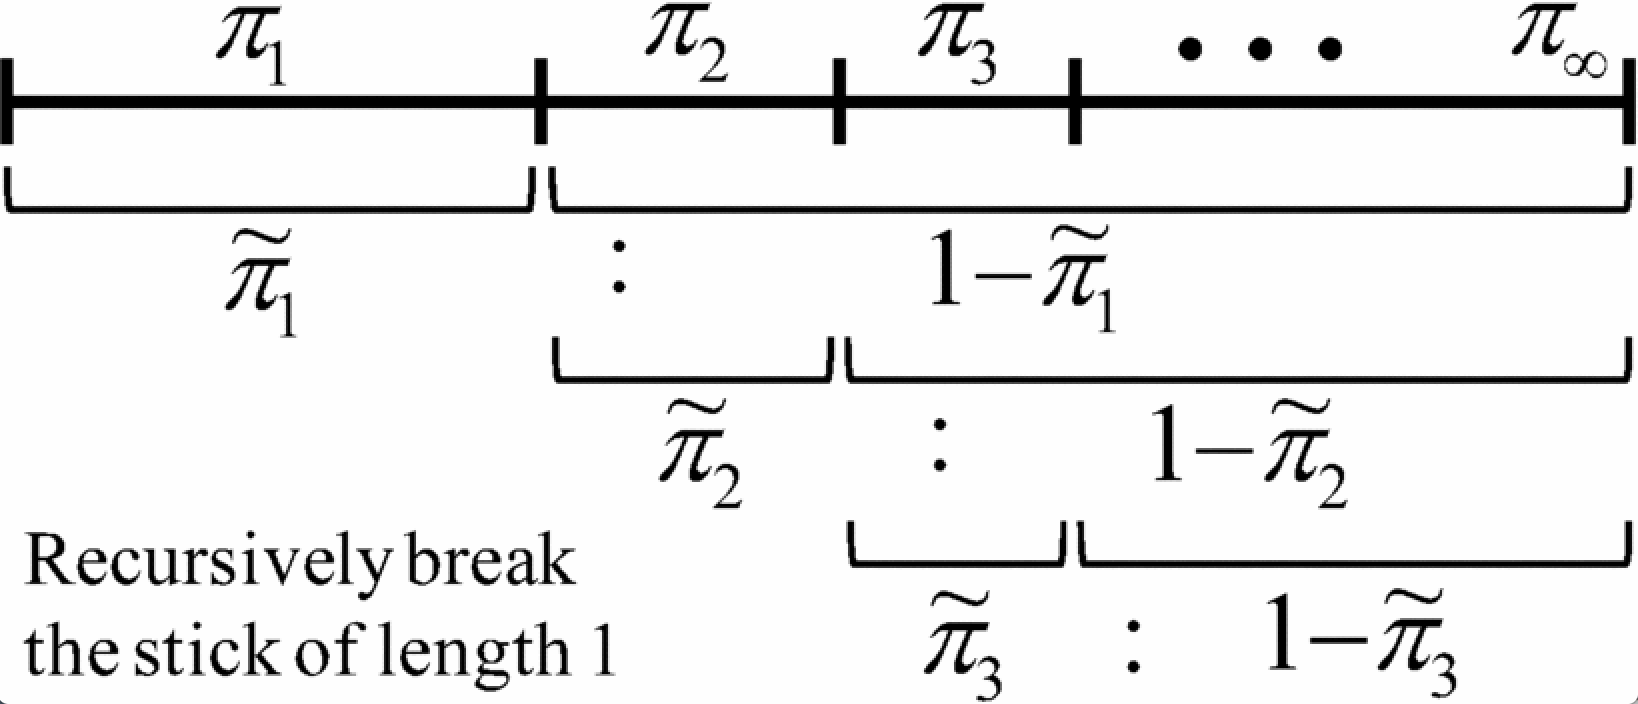
\includegraphics[width=\textwidth]{figures_julyan/intro_DP/sb}}
\end{minipage}\hskip.5cm
\begin{minipage}{.4\textwidth}
\visible<5->{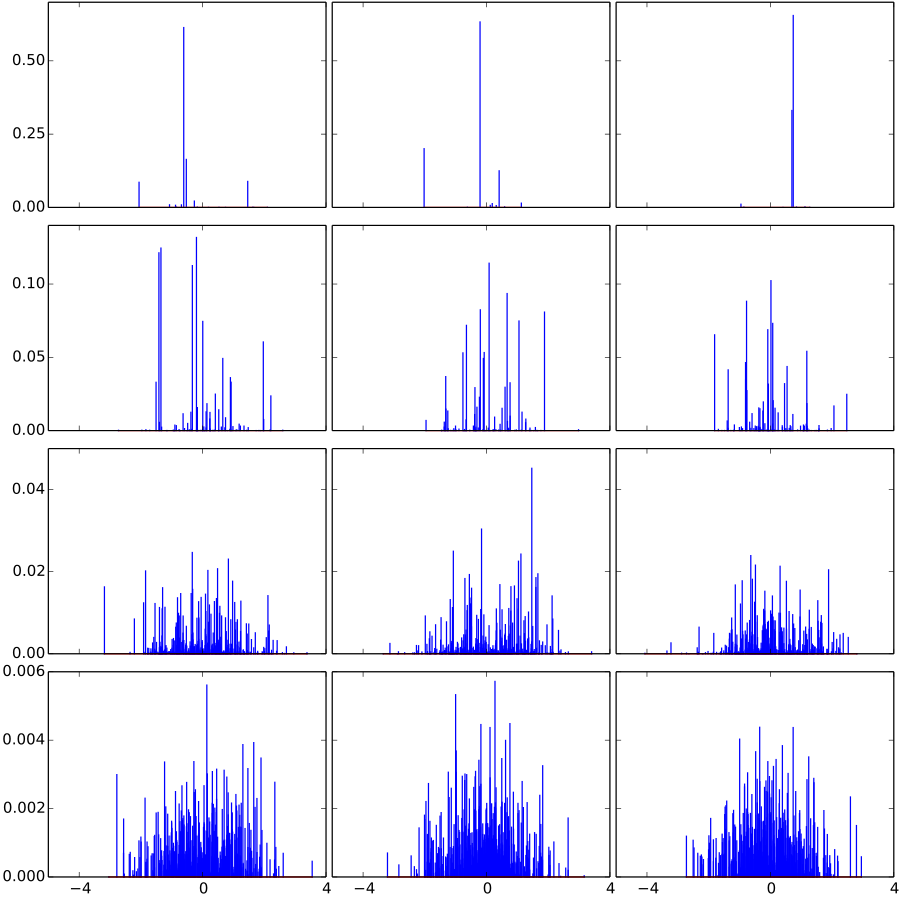
\includegraphics[width=\textwidth]{figures_julyan/intro_DP/DP}}
%\visible<5->{\includegraphics[width=\textwidth]{figures_julyan/intro_DP/SB-1}}
%\visible<6->{\includegraphics[width=\textwidth]{figures_julyan/intro_DP/SB-2}}
%\visible<7->{\includegraphics[width=\textwidth]{figures_julyan/intro_DP/SB-3}}
%\visible<8->{\includegraphics[width=\textwidth]{figures_julyan/intro_DP/SB-4}}
\end{minipage}
%($\delta_{\theta_{j}}$ stands for the Dirac mass at point $\theta_{j}$)

\end{frame}

\begin{frame}[allowframebreaks]{Stick-breaking representation}

A constructive representation of the DP due to \citet{sethuraman1994constructive}.
\begin{theorem}[Stick-breaking]\label{theorem:sethuraman}
If $V_1, V_2, \ldots \simiid Be(1, \PrecisonParam)$ and $\phi_1, \phi_2, \ldots \simiid P_0$ are i.i.d. variables, then define $p_1=V_1$ and 

$$
p_j=V_j \prod_{1\leq l \leq j}(1-V_l)
$$ 
then 
$$
P=\sum_{i=1}^\infty p_i\delta_{\phi_i}\sim \text{DP}(\PrecisonParam, P_0).
$$
\end{theorem}

\pause

\begin{lemma}
For independent $\phi\sim P_0$ and $V\sim Be(1,\PrecisonParam)$ the DP is the only solution of the distributional equation 
\begin{equation*}\label{Dir:distributional_equation}
    P \sim V\delta_\phi + (1-V)P, 
\end{equation*}
where $P\sim \text{DP}(\PrecisonParam, P_0)$.
\end{lemma}

%We say that such a RPM is solution of (\ref{Dir:distributional_equation}) if $P$ is independent of $(V, \phi)$ and if for every measurable partition $(A_1, \ldots, A_k)$ of $X$ both sides of (\ref{Dir:distributional_equation}) are random vectors equal in distribution in $\mathbb{R}^k$. 
%Proof of the lemma follows from properties of Dirichlet distribution. We are ready now to prove the  theorem.

\framebreak

\textbf{Proof.}
1) The weights $(p_1, p_2,\ldots)$ need to form a probability vector. The leftover mass at stage $j$ is 
$$
1-\bigg(\sum_{i=1}^j p_i\bigg)=\prod_{i=1}^j(1-V_i) =: R_j.
$$
One may notice that $R_j$ is decreasing and for every $j$ we have $R_j\in [0,1]$, hence we obtain almost sure convergence which is equivalent with convergence in mean. Therefore
$$
\E R_j=\E \prod_j (1-V_j)= \prod_j \E(1-V_j) = \bigg( \frac{\PrecisonParam}{\PrecisonParam + 1}\bigg)^j \rightarrow 0.
$$
So ($p_1, \ldots$) is a probability vector almost surely and $P$ is a probability measure almost surely. 

\framebreak

2) Now one may write 
$$
P=p_1\delta_{\phi_1}+\sum_{j=2}^\infty p_j\delta_{\phi_j} = V_1\delta_{\phi_1}+(1-V_1)\sum_{j=1}^\infty \Tilde{p_j}\delta_{\Tilde{\phi}_j},
$$
where $\Tilde{p}_j=\frac{p_{j+1} }{1-V_1}=V_{j+1}\prod_{l=2}^j(1-V_l)$ and $\Tilde{\phi}_j=\phi_{j+1}$, then $(\Tilde{p}_j)$ and $(\Tilde{\phi}_j)$ satisfy the same distributional definitions as $(p_j)$ and $(\phi_j)$, hence $\Tilde{P}\sim P$ and so $P$ is solution of the Lemma equation (\ref{Dir:distributional_equation}) whose only solution is the DP.
\hfill $\square$
\end{frame}






%------------
% Normalization
\begin{frame}[allowframebreaks]{DP as a normalized Gamma process}
The DP can be obtained by \alert{normalizing a Gamma process}. It is a generic way to obtain random probability measures from almost surely finite random measures. Let us restrict to $\mathcal{Y}=\mathbb{R}$.
\begin{definition}
Gamma process on $\mathbb{R}_+$ is a process $(S(u):u \geq 0)$ with independent increments satisfying
\begin{equation*}
    \forall u_1: 0 \leq u_1 \leq u_2:\quad S(u_2) - S(u_1)\simind Ga(u_2-u_1,1).
\end{equation*}
This ensures that the process has non-decreasing right continuous sample path $u\mapsto S(u)$.
\end{definition}

\begin{theorem}
For every $\PrecisonParam>0$ and for every cumulative distribution function $G$, a random cumulative distribution function such that
\begin{equation*}
    F(t) = \frac{S(\PrecisonParam G(t))}{S(\PrecisonParam)}
\end{equation*}
is the distribution of a $\mathsf{DP}(\PrecisonParam,G)$.
\end{theorem}

\textbf{Proof.}
For any set of $t_i$ satisfying $-\infty = t_0 < t_1 < \ldots < t_k = \infty$ we have 
$$
S(\PrecisonParam G(t_i)) - S(\PrecisonParam G(t_{i-1})) \sim Ga\big( \PrecisonParam G(t_i)-\PrecisonParam G(t_{i-1}),1\big).
$$
Use property that if $Y_i \simind Ga(\PrecisonParam_i, 1)$ then $(Y_1, \ldots, Y_n)/\sum_i Y_i \sim \Dir_n (\PrecisonParam_1,\ldots, \PrecisonParam_n)$ to obtain 
$$
\big(F(t_1)-F(t_0), \ldots, F(t_k) - F(t_{k-1}) \big) \sim \Dir_k\big(\PrecisonParam G(t_1) -\PrecisonParam G(t_0), \ldots, \PrecisonParam G(t_k) -\PrecisonParam G(t_{k-1})\big).
$$
Hence the definition of DP holds for every partition in intervals. These form a measure determining class, so that the definition holds for every partition in general. \hfill $\square$

\end{frame}






%------------
% P\'olya Urn charact
\begin{frame}{Definition via the P\'olya urn scheme}
A P\'olya sequence with parameter $\PrecisonParam P_0$ is a sequence of random variables $X_1, \ldots, X_n$ whose joint distribution satisfies
\begin{equation*}
    X_1 \sim P_0,\ X_{n+1}|X_1,\ldots,X_n\sim \frac{\PrecisonParam}{\PrecisonParam + n}P_0 + \frac{1}{\PrecisonParam + n}\sum_{i=1}^n \delta_{X_i}.
\end{equation*}\pause

\begin{theorem}
If $X_1,X_2,\ldots $ is a P\'olya sequence then exists random probability measure $P$ such that $X_i|P\simiid P$ and $P\sim \text{DP}(\PrecisonParam, P_0)$.
\end{theorem}\pause

\textbf{Proof.}
We can consider P\'olya sequence as an outcome of P\'olya urn, we see that it is exchangeable. By de Finetti theorem exists such probability measure $P$ such that $X_i|P \simiid P$. So far we have proved existence of the DP and know that DP generates a P\'olya sequence. Since the RPM given by de Finetti's theorem is unique this proves that
$P\sim \text{DP}(\PrecisonParam, P_0)$.\hfill $\square$

\end{frame}








\subsection[Mixture models]{Mixture models and model-based clustering}

\begin{frame}{Parametric mixtures}
 A mixture model with $K$ components has the form
 $$p(X|\pi,\phi) = \sum_{k=1}^K \pi_k p(x|\phi_k),$$
where the vector of weights $\pi = (\pi_1,\ldots,\pi_K)$ is a probability vector.

It mixes the parametric kernel (density) $p(\cdot|\phi)$ with the mixing measure
	
$$G = \sum_{k=1}^K \pi_k \delta_{\phi_k},$$
	
where $\delta_{\phi_k}$ is a point mass (Dirac Measure) at ${\phi_k}$.
	
\begin{center}
		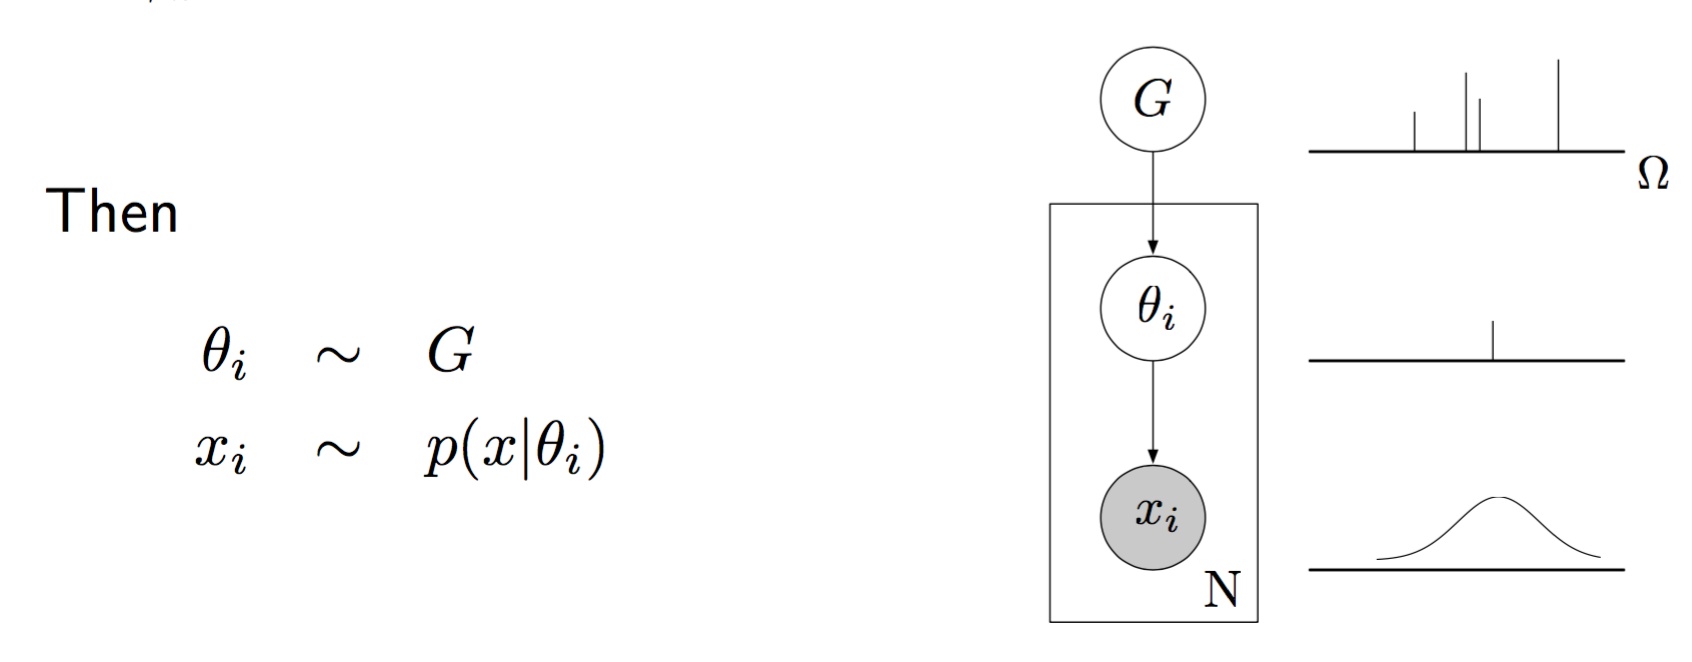
\includegraphics[width=.8\textwidth]{figures_julyan/mixtures/plate_mixture}
\end{center}
\end{frame}



\begin{frame}{Bayesian parametric mixtures}
	 For \alert{Bayesian}   mixture models, we need a distribution over the probability measure $G$, that is a distribution over weights $\pi = (\pi_1,\ldots,\pi_K)$ and over cluster-specific parameters $\phi_k$ (eg mean and covariance  $\phi_k = (\mu_k,\Sigma_k)$):

\begin{itemize}
	\item $\pi\sim \text{Dir}(\alpha/K, \ldots,\alpha/K)$
	\item $(\mu_k,\Sigma_k)\sim \text{Normal}\times\text{Inverse-Wishart}$
\end{itemize}
This makes $G = \sum_{k=1}^K \pi_k \delta_{\phi_k}$ a random probability measure (with finitely many atoms).

\begin{center}
		\includegraphics[width=.8\textwidth]{figures_julyan/mixtures/plate_bayes_mixture}
\end{center}
\end{frame}

\begin{frame}{Choosing the number of components $K$}
There are several options for choosing the \alert{number of components} $K$
\begin{itemize}
	\item Model selection with  \alert{information criteria}: AIC, BIC, or cross-validation, etc
	\item  \alert{Hierarchical model}, with a prior on $K$
	\item  \alert{Nonparametric model}, and let $K$ get large... or even possibly infinite. 
\end{itemize}
	
\end{frame}



\begin{frame}{A {Bayesian nonparametric} approach}
	 \alert{Bayesian nonparametric}   mixture models.
	 
	 We now move to $G$ being an infinite sum $G = \sum_{k=1}^\infty \pi_k \delta_{\phi_k}$ 
	
We need a distribution over this infinite random probability measure $G$. This is exactly what the \alert{Dirichlet process} does. It is parameterized by a precision parameter $\alpha$ and a base measure $G_0$.

\begin{columns}
\column{.45\textwidth}
\begin{itemize}
	\item $\pi = (\pi_1,\pi_2,\ldots)\sim \text{GEM}(\alpha)$
	\item $\phi_k\simiid G_0$
\end{itemize}

\column{.45\textwidth}
\begin{center}
		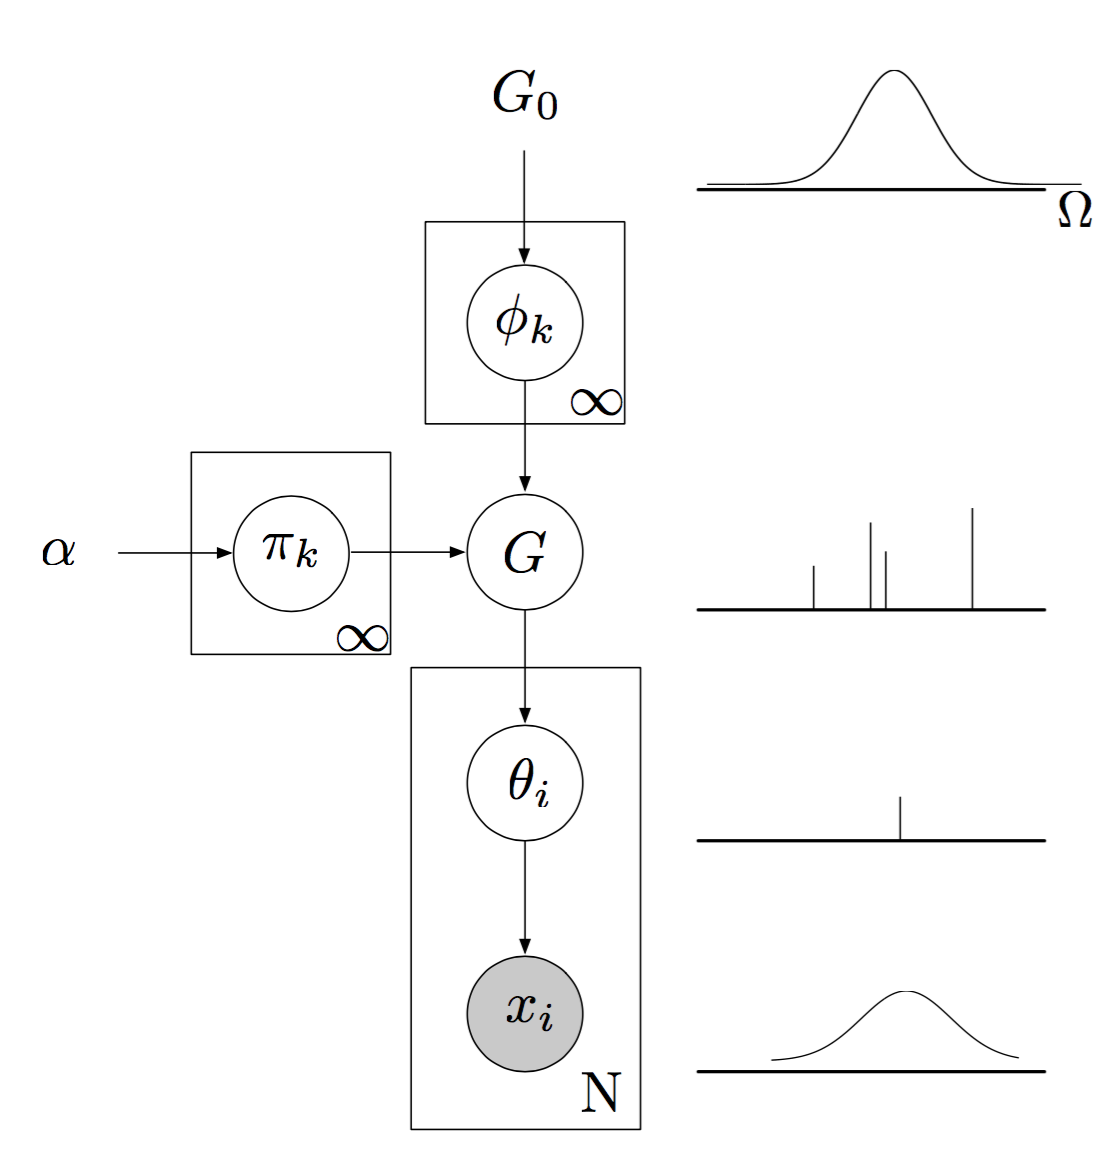
\includegraphics[height=.4\textheight]{figures_julyan/mixtures/plate_SB_mixture}
\end{center}
\end{columns}
\end{frame}



\begin{frame}{Posterior sampling}
Markov chain Monte Carlo (MCMC) methods:
\begin{itemize}
\item \alert{Marginal methods}: marginalizing over the posterior DP $P$, and sampling using the posterior P\'olya urn scheme \citep[easy in conjugate case, see][]{neal2000markov}
\item \alert{Conditional methods}: sampling a finite but sufficient number of parameters
 \citep{ishwaran2001gibbs}. \alert{BNPdensity} R package \citep{arbel2021BNPdensity}.
\end{itemize}
Variational approximations \citep{blei2006variational}
\end{frame}



\begin{frame}[allowframebreaks]{Warning on interpretation of $K_n$}
\begin{columns}

\column{.45\textwidth}

	Consider a simple DP mixture model with
	\begin{itemize}
		\item  Gaussian base measure, 
		\item Gaussian kernel,
		\item where data are sampled  iid from some distribution.
	\end{itemize}
	
Then the \alert{posterior on $K_n$ is inconsistent} \citep{miller2013simple}.
\column{.45\textwidth}
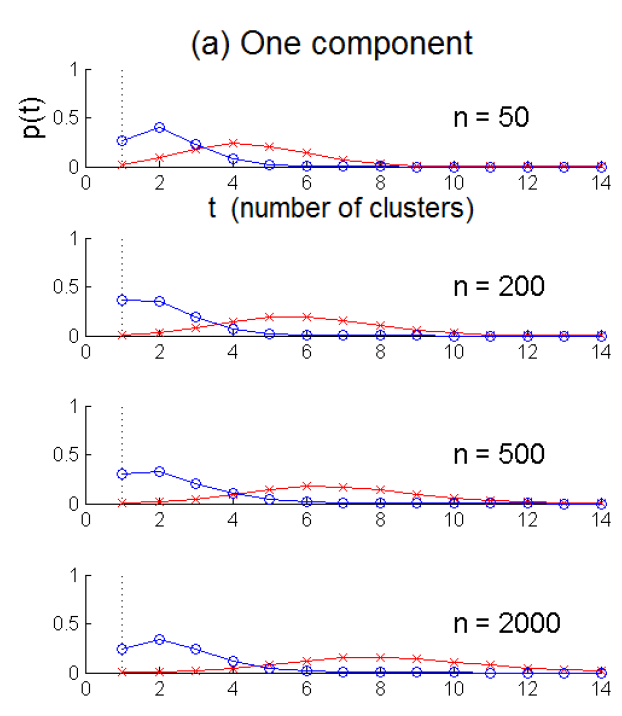
\includegraphics[width=\textwidth]{figures_julyan/mixtures/miller_DP}
\end{columns}
\framebreak

From \citet{miller2013simple} (here $K_n$ is denoted $T_n$):\bigskip

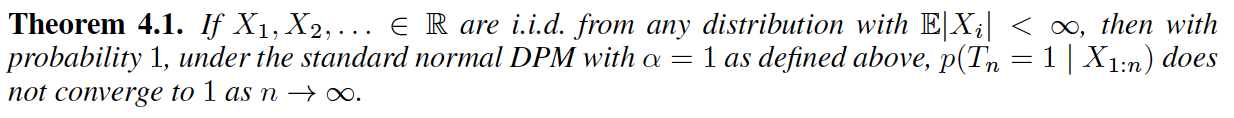
\includegraphics[width=\textwidth]{figures_julyan/mixtures/miller_inconsistency1}\bigskip

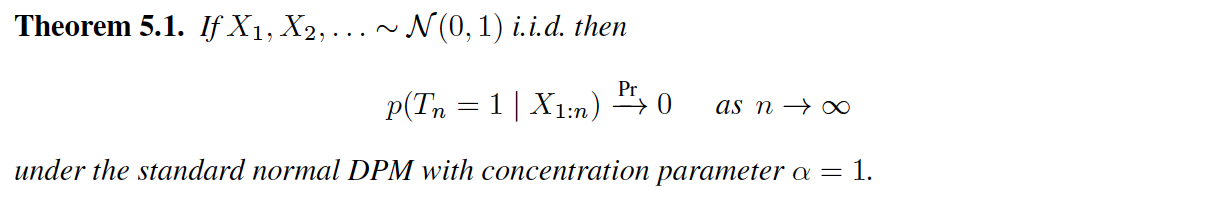
\includegraphics[width=\textwidth]{figures_julyan/mixtures/miller_inconsistency2}\bigskip


But there is some hope...
\end{frame}



\begin{frame}{Bayesian decision theory}
	From decision theory: a Bayes estimator minimizes a posterior expected loss.
	
\begin{equation*}
\hat{a}_L = \arg \inf_{a \in A} \mathbb{E}_{\pi(\theta)}[L_a(\theta)].
\end{equation*}\pause

Examples with Euclidean parameter spaces:
\begin{itemize}
	\item $L^2$, squared loss $\longrightarrow$ posterior mean
	\item $L^1$, absolute loss $\longrightarrow$ posterior median
	\item $0-1$ loss  $\longrightarrow$ mode a posteriori (MAP)
\end{itemize}
\end{frame}

\begin{frame}{Deriving an optimal clustering}

The posterior expected loss of clustering $c'$, denoted by $L(c')$, is obtained by \alert{averaging the loss with respect to posterior weights}
$$L(c') = \sum_{c\in\Ac_n} L(c,c')p(c|\bx),$$
and the decision is taken by choosing the best

\begin{equation*}
\hat c = \arg \min_{c' \in \Ac_n} \sum_{c\in\Ac_n} L(c,c')p(c|\bx)
\end{equation*}\pause
Several losses have been considered:
	\begin{itemize}
		\item 0-1 loss \citep{rajkowski2019analysis},
		\item Binder loss \citep{dahl2006model},
		\item Variation of information \citep{wade2018bayesian}.
	\end{itemize}
\end{frame}

\begin{frame}{Simplest loss: $L_{0-1}$}

\begin{align*}
	L_{0-1}(c') = \sum_{c\in\Ac_n} L_{0-1}(c,c')p(c|\bx) &= \sum_{c\in\Ac_n,\,c\neq c'} p(c|\bx),\\
	& = 1 - p(c'|\bx)\pause
\end{align*}
which is to say that the expected loss of $c'$ is \alert{all the posterior mass except that of $c'$.} So that it is easily minimized at the value $c'$ which has \alert{maximum} posterior weight:
$$\hat c =  \arg \min_{c' \in \Ac_n} L_{0-1}(c') =   \arg \max_{c' \in \Ac_n} p(c'|\bx):= MAP.$$\pause

Negative results by \citet{rajkowski2019analysis} show that the \alert{maximum a posteriori (MAP) is inconsistent}.
	
\end{frame}

%\begin{frame}{Variation of information}
%\alert{Variation of information} (VI) by \citet{meila2007comparing} for cluster comparison. From information theory, compares information in two clusterings with information shared between the two clusterings:
%\begin{align*}
%&\VI(\bc,\widehat{\bc})=\En(\bc)+\En(\widehat{\bc})-2\I(\bc,\widehat{\bc})
%\end{align*}
%\end{frame}
%
%
%\begin{frame}{Variation of information}
%\citet{wade2018bayesian} 
%compare Binder and VI:\bigskip
%
%\begin{center}
%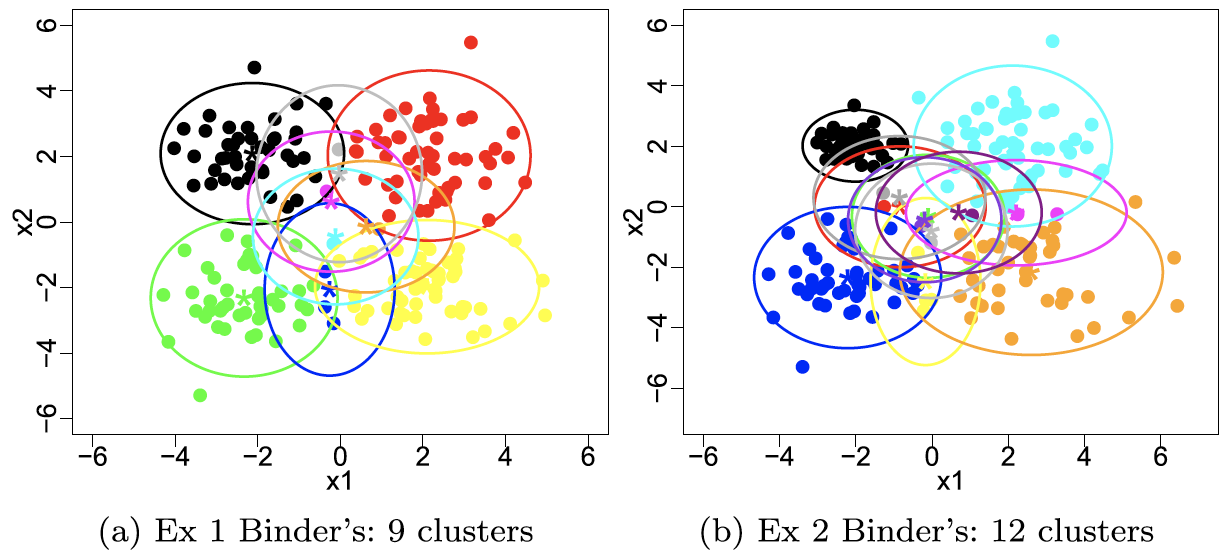
\includegraphics[width=.7\textwidth]{figures_julyan/mixtures/wade_example_binder}
%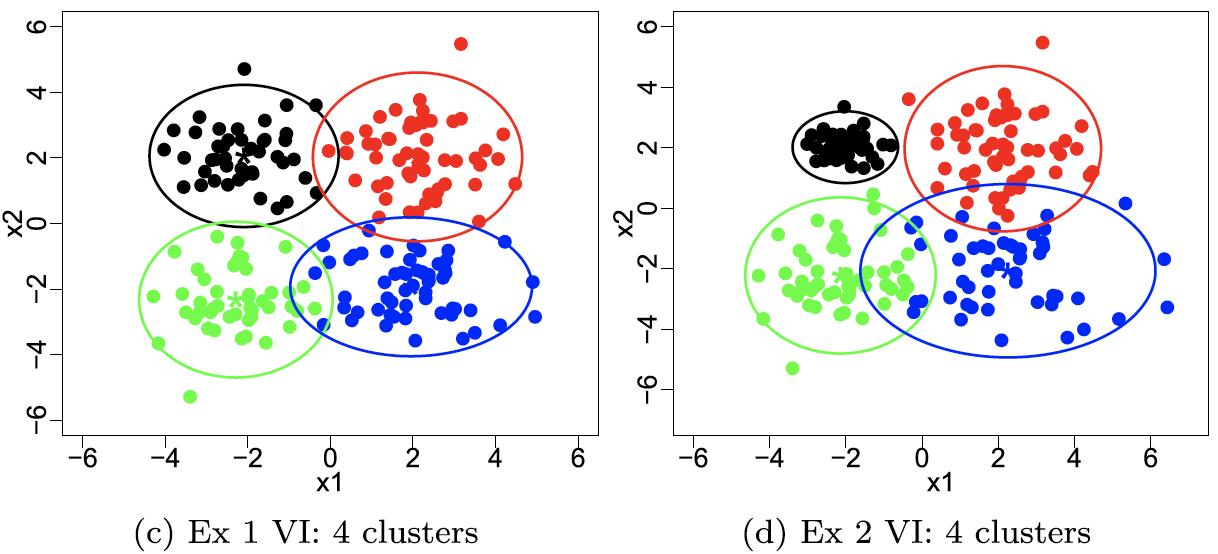
\includegraphics[width=.7\textwidth]{figures_julyan/mixtures/wade_example_VI}	
%\end{center}
%\end{frame}
%
%
%\begin{frame}{Variation of information}
%\citet{wade2018bayesian} 
%also provide \alert{credible balls} around the estimated clustering, based on Hasse diagram:\bigskip
%
%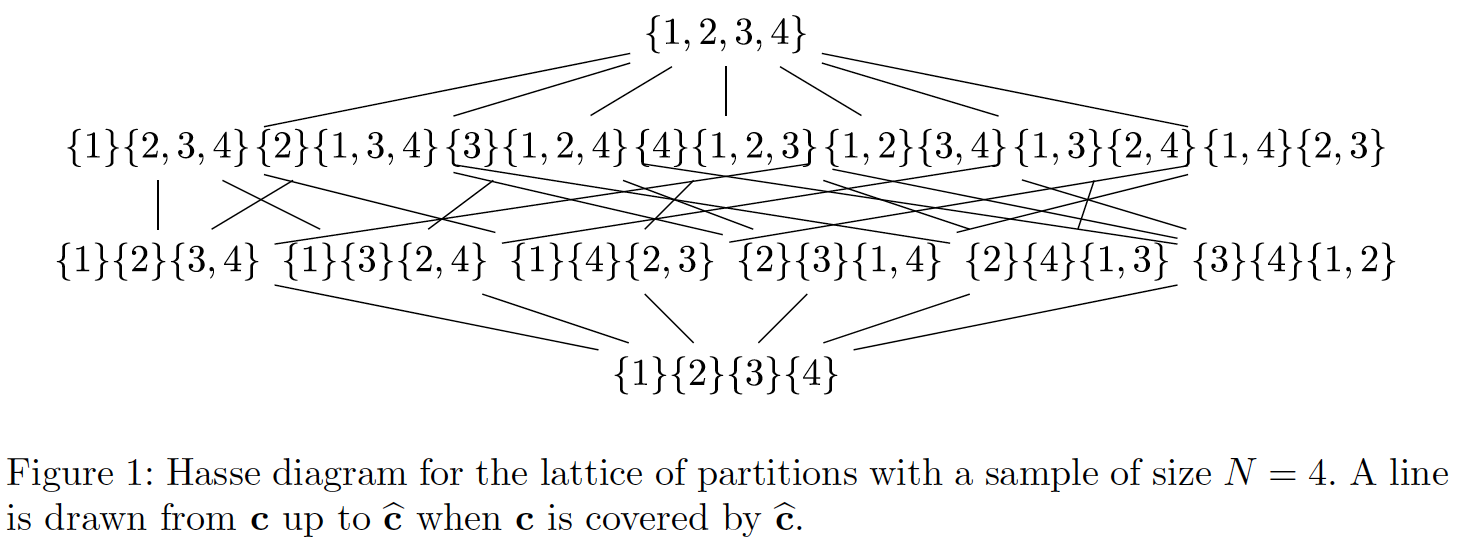
\includegraphics[width=\textwidth]{figures_julyan/mixtures/hasse_diagram}
%\end{frame}


 \subsection[Other priors]{Priors beyond the DP}
 
 \begin{frame}{Need for a power-law for $K_n$}
 	\citet{newman2005power,clauset2009power} show that ``\textit{Power-law distributions occur in many situations of scientific interest and have
significant consequences for our understanding of natural and man-made phenomena}''.
		\visible<2->{
		\begin{center}
			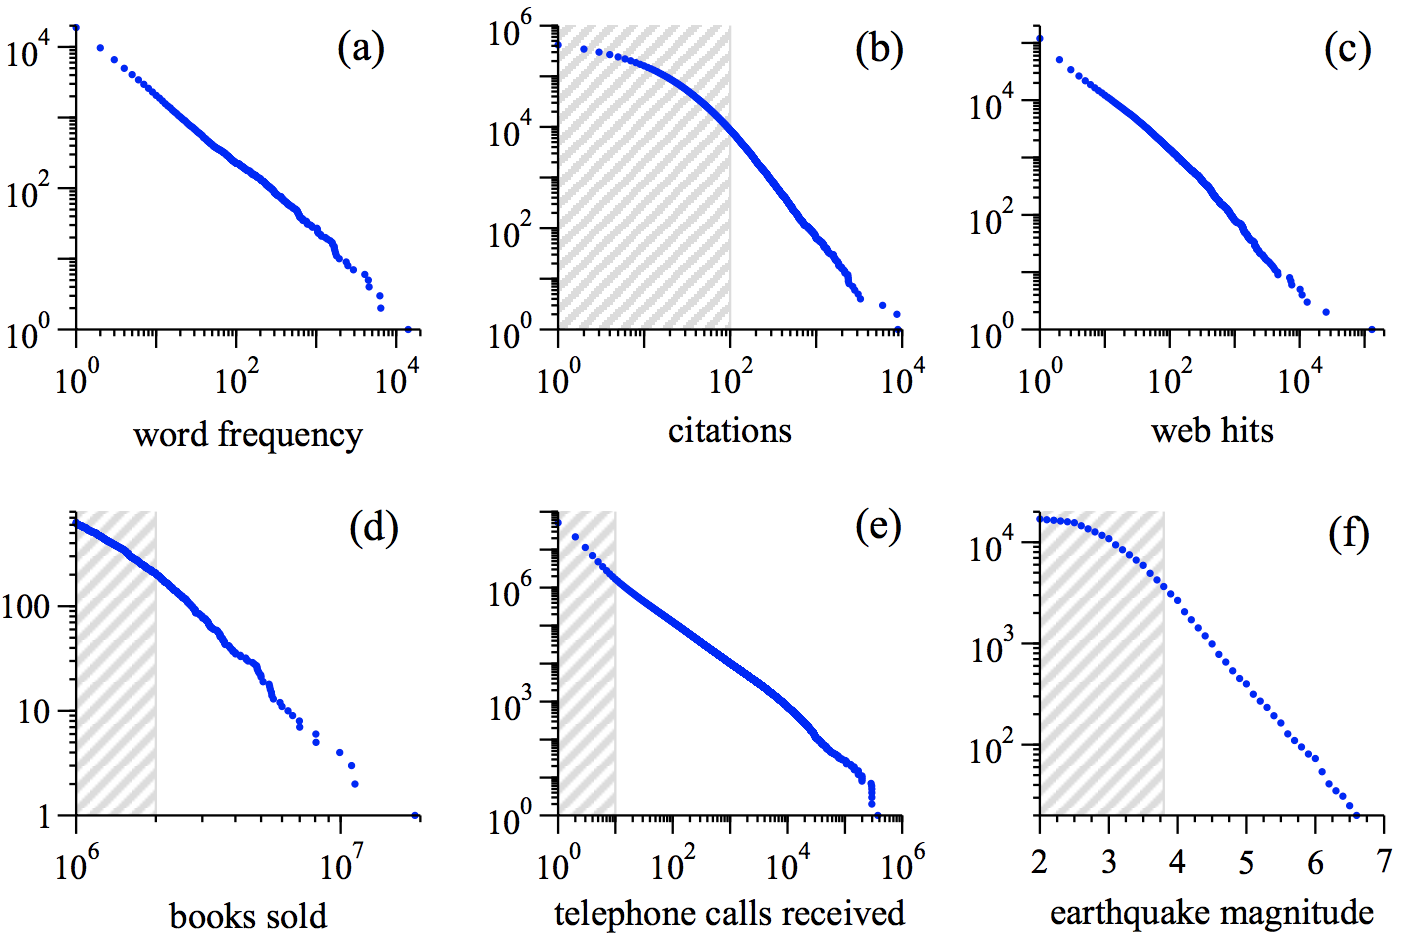
\includegraphics[width=.7\textwidth]{figures_julyan/beyond_DP/power_laws_newman}
		\end{center}
		\hfill\textcolor{gray}{[Image from \citet{newman2005power}]}\\
		}\pause
		Hence the need to depart from $K_n\sim \alpha \log n$ induced by a Dirichlet process.
 \end{frame}

 
\begin{frame}{Chinese restaurant process}
Consider discrete data $X_1,\ldots X_n\vert P\simiid P$, and $ P \sim \mathcal{Q}$

Features $k_n\leq n$ unique values $X_1^*,\ldots,X_{k_n}^*$ with resp. frequencies $n_1,\ldots,n_{k_n}$\medskip 


{Discrete random probability measures} are characterized by  \alert{predictive distr.}
\medskip

\only<1>{\alert{Dirichlet process} by \citet{ferguson1973bayesian}: $P\sim DP(\alpha, G_0)$

$$\P[X_{n+1}\in \cdot\, \vert\, X_1,\ldots X_{n}]=\frac{\alpha}{\alpha+n}G_{0}(.)+\frac{1}{\alpha+n}\sum_{j=1}^{{k_n}}n_j\delta_{X_{j}^*}(.)$$

\begin{center}
Log rate for number of clusters \alert{$k_n \asymp \alpha \log n$}
\end{center}

\medskip

\textcolor{gray}{
Product form exchangeable partition probability function  
$$p(n_1,\ldots,n_{k_n})=\alpha^{k_n}\frac{\Gamma(\alpha)}{\Gamma(\alpha+k_n)}\prod_{j=1}^{k_n}(n_j-1)!$$}
}


\only<2>{\alert{Pitman--Yor process} by \citet{pitman1997two}: $P\sim PY(\alert{\sigma},\alpha, G_0),\,\sigma\in(0,1)$

$$\P[X_{n+1}\in \cdot\, \vert\, X_1,\ldots X_{n}]=\frac{\alpha+\alert{\sigma k_n}}{\alpha+n}G_{0}(.)+\frac{1}{\alpha+n}\sum_{j=1}^{{k_n}}(n_j-\alert{\sigma})\delta_{X_{j}^*}(.)$$

\begin{center}
Power law rate for number of clusters \alert{$k_n \asymp S n^\sigma$}
\end{center}

\medskip

\textcolor{gray}{
Product form exchangeable partition probability function  
$$p(n_1,\ldots,n_{k_n})=\frac{\prod_{i=1}^{k_n-1}(\alpha+i\sigma)}{(\alpha+1)_{(n-1)}}\prod_{j=1}^{k_n}(1-\sigma)_{(n_j-1)}$$}
}


\only<3>{\alert{Gibbs-type processes} by \citet{pitman2003poisson}: $P\sim Gibbs(\alert{\sigma},(V_{n,k})_{n,k}, G_0),\,\sigma<1$

$$\P[X_{n+1}\in \cdot\, \vert\, X_1,\ldots X_{n}]=\alert{\frac{V_{n+1,{k_n}+1}}{V_{n,{k_n}}}}G_{0}(.)+\alert{\frac{V_{n+1,{k_n}}}{V_{n,{k_n}}}}\sum_{j=1}^{{k_n}}(n_j-\alert{\sigma})\delta_{X_{j}^*}(.)$$

\begin{center}
Rate for number of clusters 
$\alert{k_n \asymp }
\left\{
\begin{array}{l}
\alert{K} \text{ random variable a.s. finite if }\sigma<0\\
\alert{\alpha \log n}  \text{  if }\sigma=0\\
\alert{S n^\sigma} \text{ if }\sigma\in(0,1), (S \text{ random variable)}.
\end{array}
\right.
$
\end{center}
\medskip

\textcolor{gray}{
Product form exchangeable partition probability function  
$$p(n_1,\ldots,n_{k_n})=V_{n,{k_n}}\prod_{j=1}^{k_n}(1-\sigma)_{(n_j-1)}$$}
}
\end{frame}



\begin{frame}{Beyond the DP from predictive function viewpoint} 
%According to the de Finetti representation theorem, $(X_{i})_{i\geq1}$ is an exchangeable sequence. The distribution of such a sequence, and hence $\mathscr{Q}$, is 
%characterized by conditional probability of discovering a new species at $(n+1)$-th step, i.e.
%\vspace{0.1cm}
%\begin{equation}\label{eq:newspecies} \tag{$\ast$}
%\P[X_{n+1}\hbox{ is ``new''} \: |\: \boldsymbol{X}_{n}].
%\end{equation}

A discrete random probability measure $P$ can be classified in 3 main categories according to $\P[X_{n+1}\hbox{ is ``new''} \: |\: \boldsymbol{X}_{n}]$
    \begin{itemize}
    \smallskip
    \item<2->[1)] $\P[X_{n+1}\hbox{ is ``new''} \: |\: \boldsymbol{X}_{n}]=\alert{f(n, \hbox{model parameters})}$

     $ \hspace{1.2cm} \Longleftrightarrow \ $ depends on $n$ but not on $k_{n}$ and $(n_{1},\ldots,n_{k_{n}})$

     $ \hspace{1.2cm} \Longleftrightarrow \ $ Dirichlet process \citep{ferguson1973bayesian};\\[4pt]
     
    \smallskip

    \item<3->[2)] $\P[X_{n+1}\hbox{ is ``new''} \: |\: \boldsymbol{X}_{n}]=\textcolor{red2}{f(n, k_{n}, \hbox{model parameters})}$

    $ \hspace{1.2cm} \Longleftrightarrow \ $ depends on $n$ and $k_{n}$  but not on $(n_{1},\ldots,n_{k_{n}})$

    $ \hspace{1.2cm} \Longleftrightarrow \ $\textcolor{red2}{Gibbs-type prior} \citep{pitman2003poisson};\\[4pt]

\smallskip

    \item<4->[3)] $\P[X_{n+1}\hbox{ is ``new''} \: |\: \boldsymbol{X}_{n}]=\alert{f(n, k_{n}, (n_{1},\ldots,n_{k_{n}}), \hbox{model parameters})}$

    $ \hspace{1.2cm} \Longleftrightarrow \ $ depends on  $n$, $k_{n}$ and $(n_{1},\ldots,n_{k_{n}})$
    
    $ \hspace{1.2cm} \Longleftrightarrow \ $ tractability issues
    
 \end{itemize}
\end{frame}


\begin{frame}{Tree of discrete random probability measures}
\only<1>{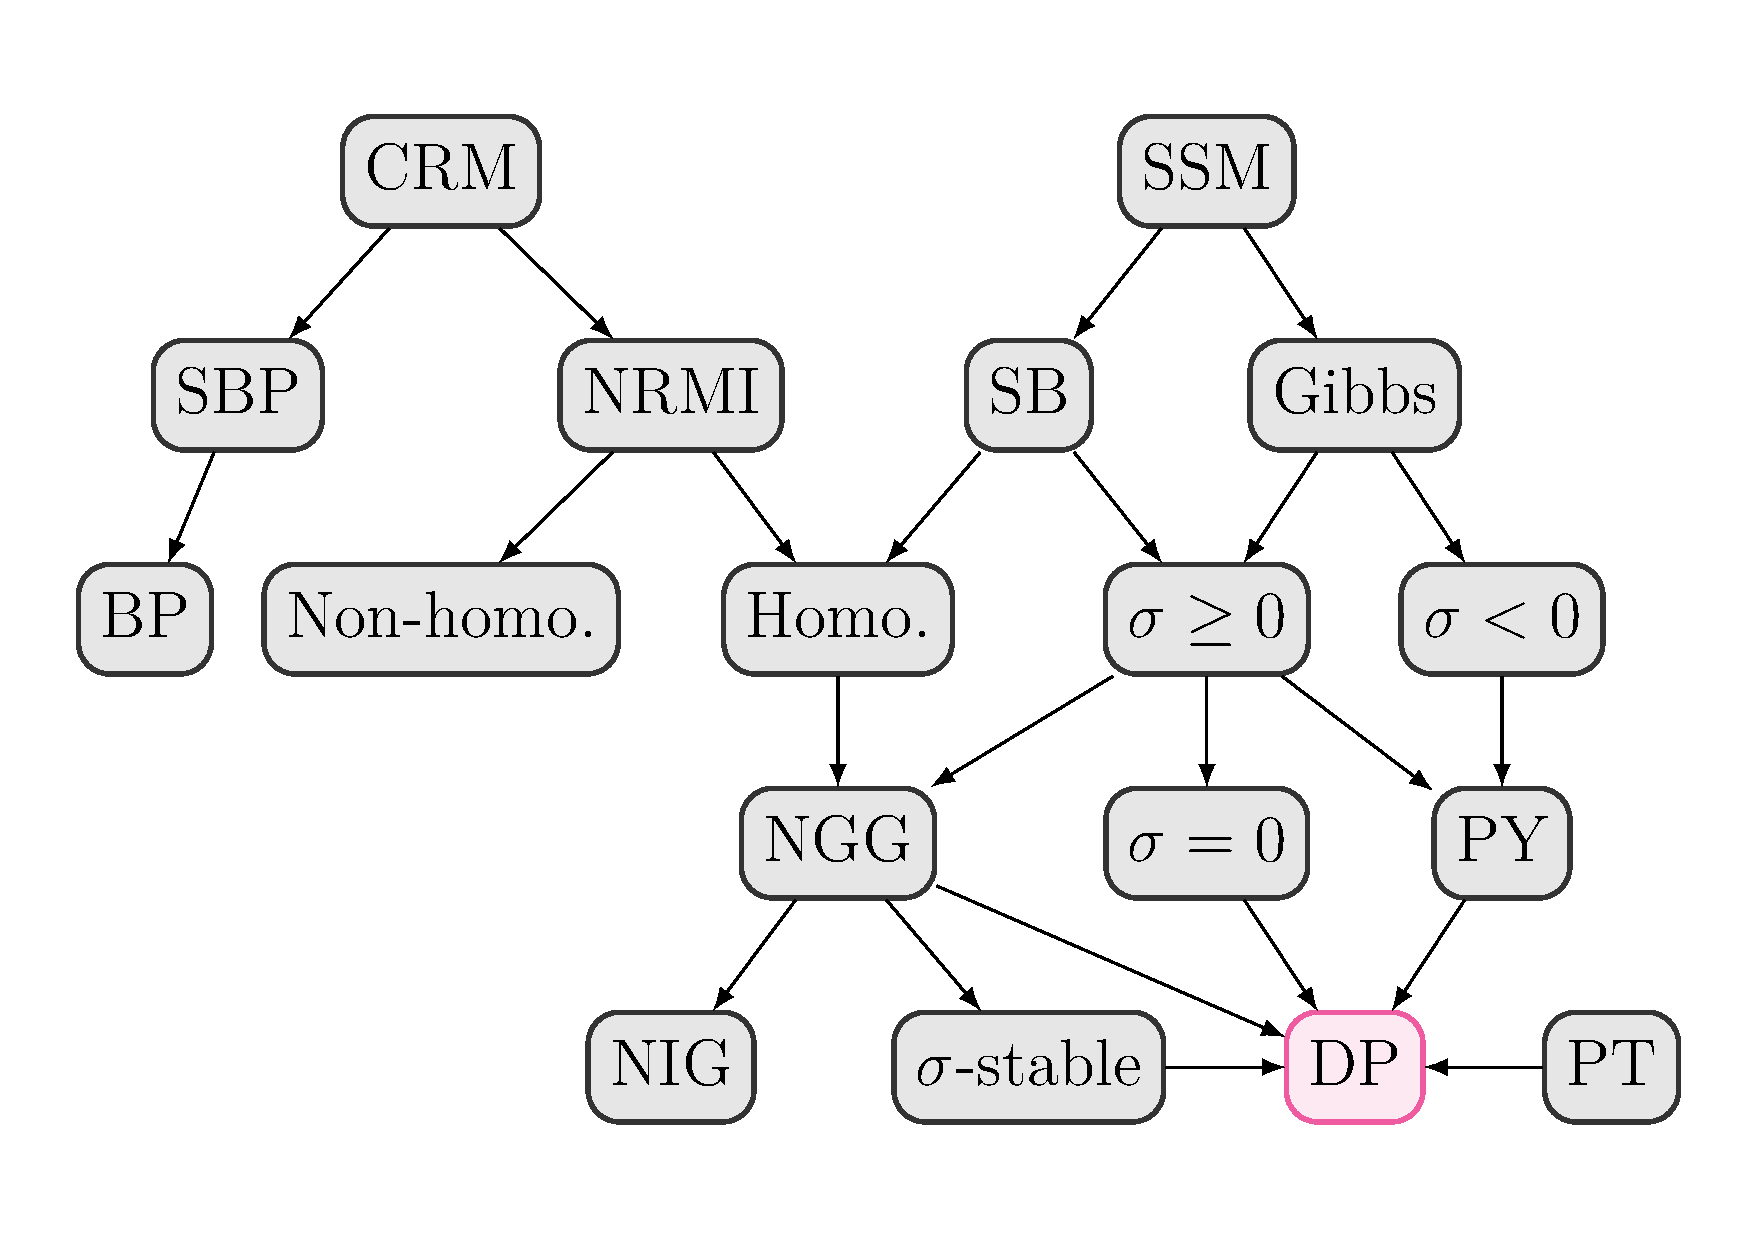
\includegraphics[width=\textwidth]{figures_julyan/introRPM/graph_model}}
\only<2>{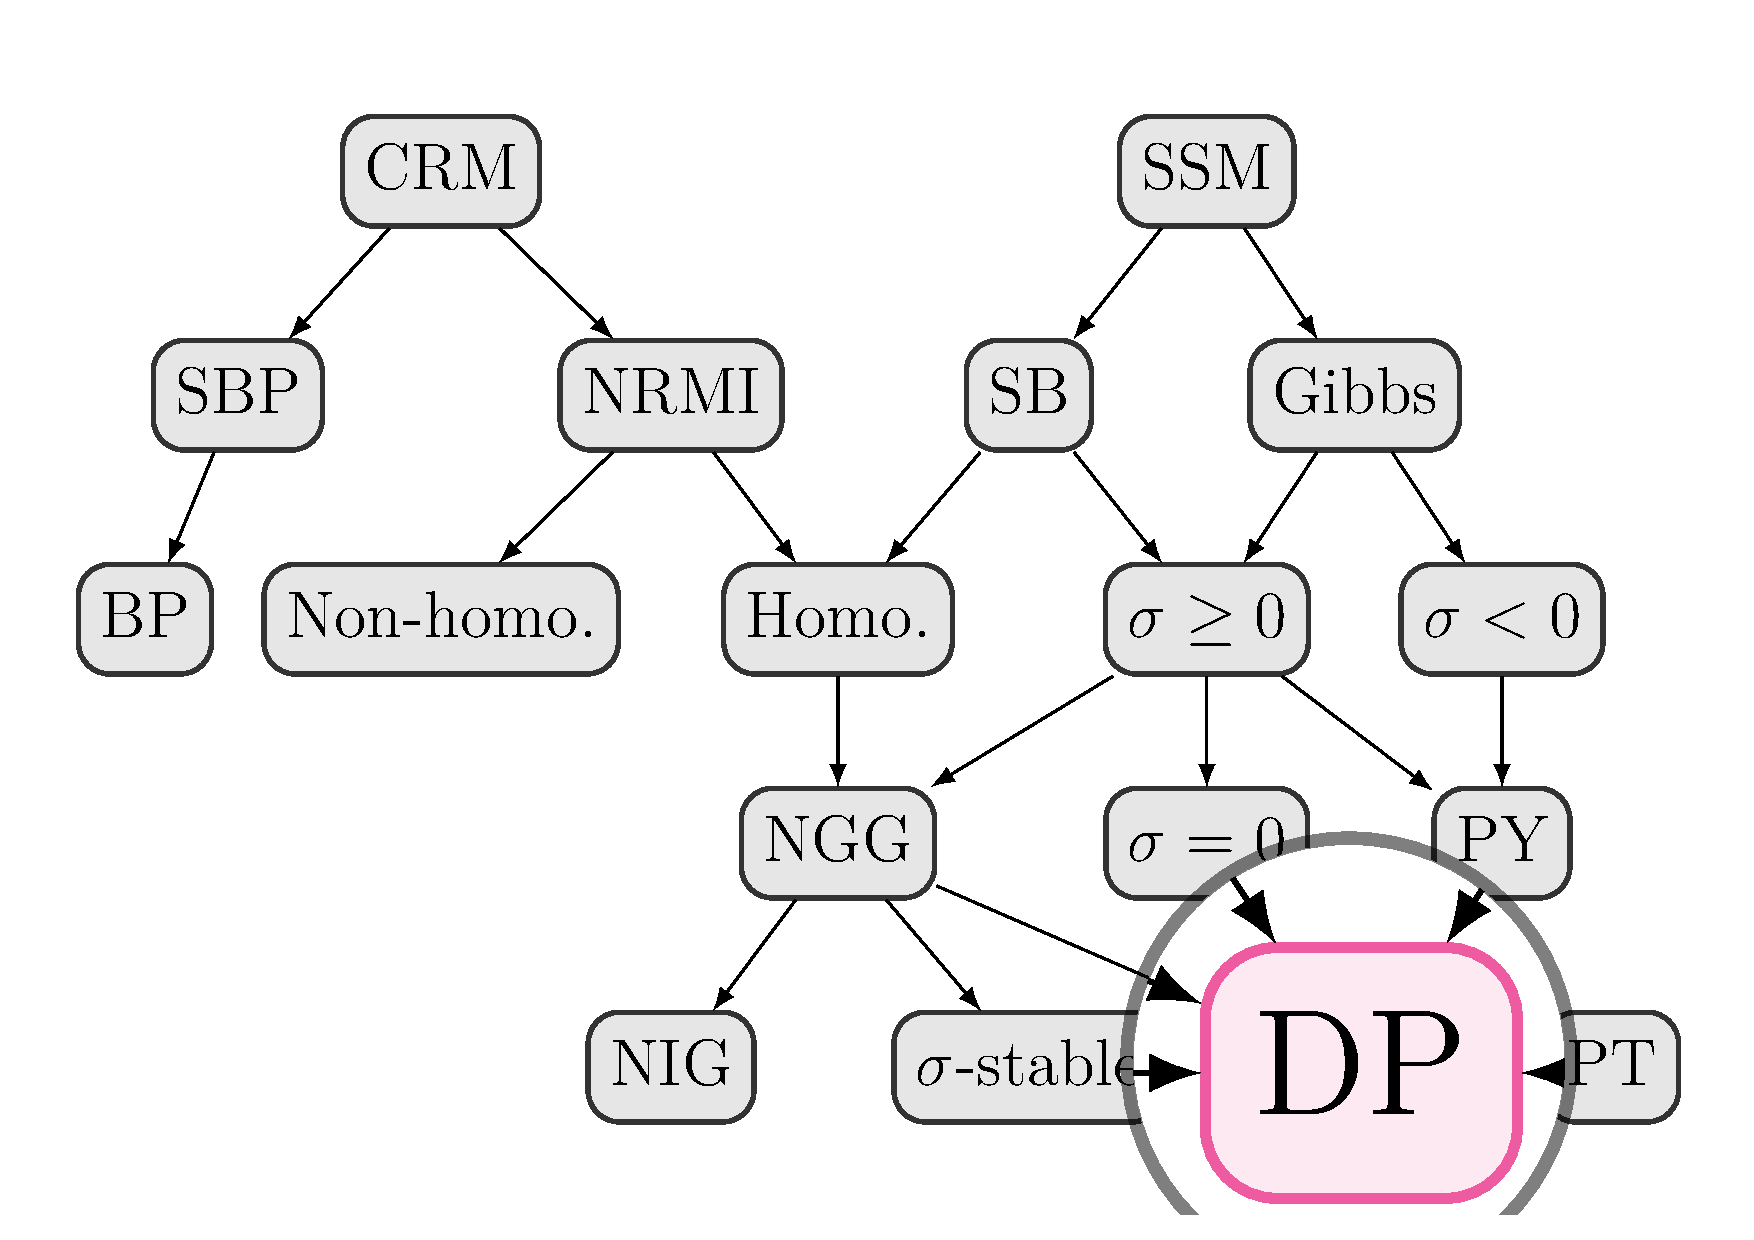
\includegraphics[width=\textwidth]{figures_julyan/introRPM/graph_model_dp}}
\end{frame}


%------------------
% PY

\begin{frame}[allowframebreaks]{Pitman--Yor process}
	\begin{proposition}
[Pitman Sampling formula] The multiplicities $(m_1,\ldots,m_n)$ in $X_1,\ldots, X_n|P\simiid P,\ P\sim PY(\sigma, \PrecisionParam, P_0)$ have distribution
\begin{equation*}
    p(m_1,\ldots,m_n)=\frac{n!}{(1+\PrecisionParam)_{(n-1)}}(\PrecisionParam +\sigma)\cdots (\PrecisionParam+(k-1)\sigma)\prod_{\ell=1}^n\frac{1}{m_\ell!}\bigg(\frac{(1-\sigma)_{(\ell-1)} }{\ell!}\bigg)^{m_\ell}
\end{equation*}
\end{proposition}


\textbf{Proof.}
Same technique as for the DP Ewens sampling formula.



\framebreak

\begin{columns}

\column{.6\textwidth}
\begin{proposition}[Power law and $\sigma$-diversity]
For $\sigma >0$ we have the almost sure convergence 
$$
n^{-\sigma}K_n\rightarrow S_{\sigma, \PrecisionParam},
$$
where $ S_{\sigma, \PrecisionParam}$ is called $\sigma$-diversity of the PY, whose density is a polynomially tilted \alert{Mittag--Leffler density} (ML):
\begin{equation*}
    g_{\sigma,\PrecisionParam}(x)\propto x^{\PrecisionParam/\sigma}g_\PrecisionParam (x),
\end{equation*}
and $g_\alpha$ is ML density.
\end{proposition}
\column{.35\textwidth}
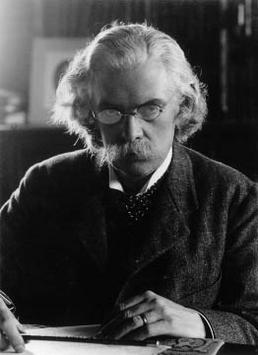
\includegraphics[width=\textwidth]{figures_julyan/trombi/Mittag-Leffler}
		\hfill\textcolor{gray}{[Image: Wikipedia]}
\end{columns}




\framebreak

\begin{theorem}[Stick breaking representation for PY]
If $V_j\simind Be(1-\sigma, \PrecisionParam + j\sigma)$ and $p_1=V_1,\ p_j=V_j\prod_{l<j}(1-V_l)$ and further we have $\phi_j\simiid P_0$ then 
$$
P=\sum_{j=1}^\infty p_j \delta_{\phi_j} \sim PY(\sigma,\PrecisionParam P_0).
$$
\end{theorem}

\framebreak


\begin{proposition}
[Moments of PY] If $P\sim PY(\sigma, \PrecisionParam, P_0)$, then for every measurable sets $A,B$ we have
\begin{enumerate}
    \item[1)] $\E [P(A)] = P_0(A),$
    \item[2)] $\E[P(A)P(B)]=(1-\sigma)/(1+\PrecisionParam)P_0(A\cap B) + (\PrecisionParam + \sigma)/(1+ \PrecisionParam)P_0(A)P_0(B),$
    \item[3)] $\Cov[P(A),P(B)] = (1-\sigma)/(1+\PrecisionParam)\big(P_0(A\cap B) -P_0(A)P_0(B)\big)$.  
\end{enumerate}
\end{proposition}
\framebreak


\alert{Proof.}
\begin{enumerate}
    \item[1)] We use the stick-breaking representation:
    \begin{equation*}
        \E P(A) =\sum_j \E p_j \E\delta_{\phi_j}=\sum_j \E(p_j) P_0(A) = P_0(A)\E (\sum_j p_j)= P_0(A).
    \end{equation*}
    \item[2)] Let $X_1, X_2|P \simiid P$, then
    \begin{equation*}
        \E(P(A)P(B)) = \P(X_1\in A, X_2\in B)=\P(X_1\in A)\P(X_2\in B|X_1\in A).
    \end{equation*}
    Lets investigate two terms above: from 1) we know that $\P(X_1\in A)=P_0(A)$. We know the predictive of PY:
    \begin{equation*}
        X_2|X_1 \sim \frac{\PrecisionParam + \sigma}{\PrecisionParam + 1}P_0+\frac{1-\sigma}{\PrecisionParam + 1}\delta_{X_1},
    \end{equation*}
    and hence
    \begin{equation*}
        \P(X_2\in B|X_1\in A) = \frac{\PrecisionParam + \sigma}{\PrecisionParam + 1}P_0(B) + \frac{1-\sigma}{\PrecisionParam + 1}P_{0A}(B),
    \end{equation*}
    when we used notation $P_{0A}(B)=P_0(B|A)=P_0(A\cap B)/P_0(A)$ for a conditional measure.
    \item[3)] It is straightforward combination of 1) and 2).
\end{enumerate}

\framebreak

Unlike the DP, the \alert{PY is not conjugate}. However, the posterior can be explicited.

\begin{theorem}
[Posterior distribution of PY] If $P\sim PY(\sigma, \PrecisionParam, P_0)$ then the posterior of $P$ based on observations $X_{1:n}|P\simiid P$ has the distribution of the random probability measure
\begin{equation*}
    (1-q_n)P_n + q_n \sum_{j=1}^{K_n}p_j^*\delta_{X_j^*},
\end{equation*}
where $X^*_{1:n}$ are the $K_n$ distinct values in $X_{1:n}$, frequencies are denoted $n_1,\ldots,n_{K_n}$ and 
\begin{itemize}
    \item $q_n\sim Beta(n-K_n \sigma, \PrecisionParam +K_n\sigma)$,
    \item $(p_1^*, \ldots, p^*_{K_n})\sim \Dir(n_1-\sigma, \ldots, n_{K_n} -\sigma)$,
    \item $P_n\sim PY(\sigma, (\PrecisionParam + \sigma K_n)P_0)$.
\end{itemize}
\end{theorem} 
\end{frame}

\begin{frame}{Impact of the stability parameter $\sigma$}
Prior distribution of the number of clusters $K_n$ 
\begin{itemize}
\item<1-> \textcolor<1>{red2}{$\alpha$ controls the location} (as for the DP)
\item<2-> \textcolor<2>{red2}{$\sigma$ controls the flatness (or variability)}
\end{itemize}
\visible<3->{
With $n=50, \alpha=1$ and \textcolor{red2}{$\sigma=0.2,0.3,\ldots, 0.8$} \textcolor{gray}{[Image from \citet{deblasi2015gibbs}]}

}
\begin{center}
\visible<3->{\adjincludegraphics[width=.7\textwidth,trim={0 {.1\height} 0 {.12\height}},clip]{figures_julyan/introRPM/prior_K_n_PY.pdf}\\
}
\end{center}
\end{frame}

\subsection{Beyond mixtures: non-exchangeable settings and feature allocation models}


\begin{frame}{Hierarchical Dirichlet process}
A nonparametric version of \alert{Latent dirichlet allocation} \citep{blei2003latent} due to  \citet{teh2006hierarchical}\\
\begin{center}
		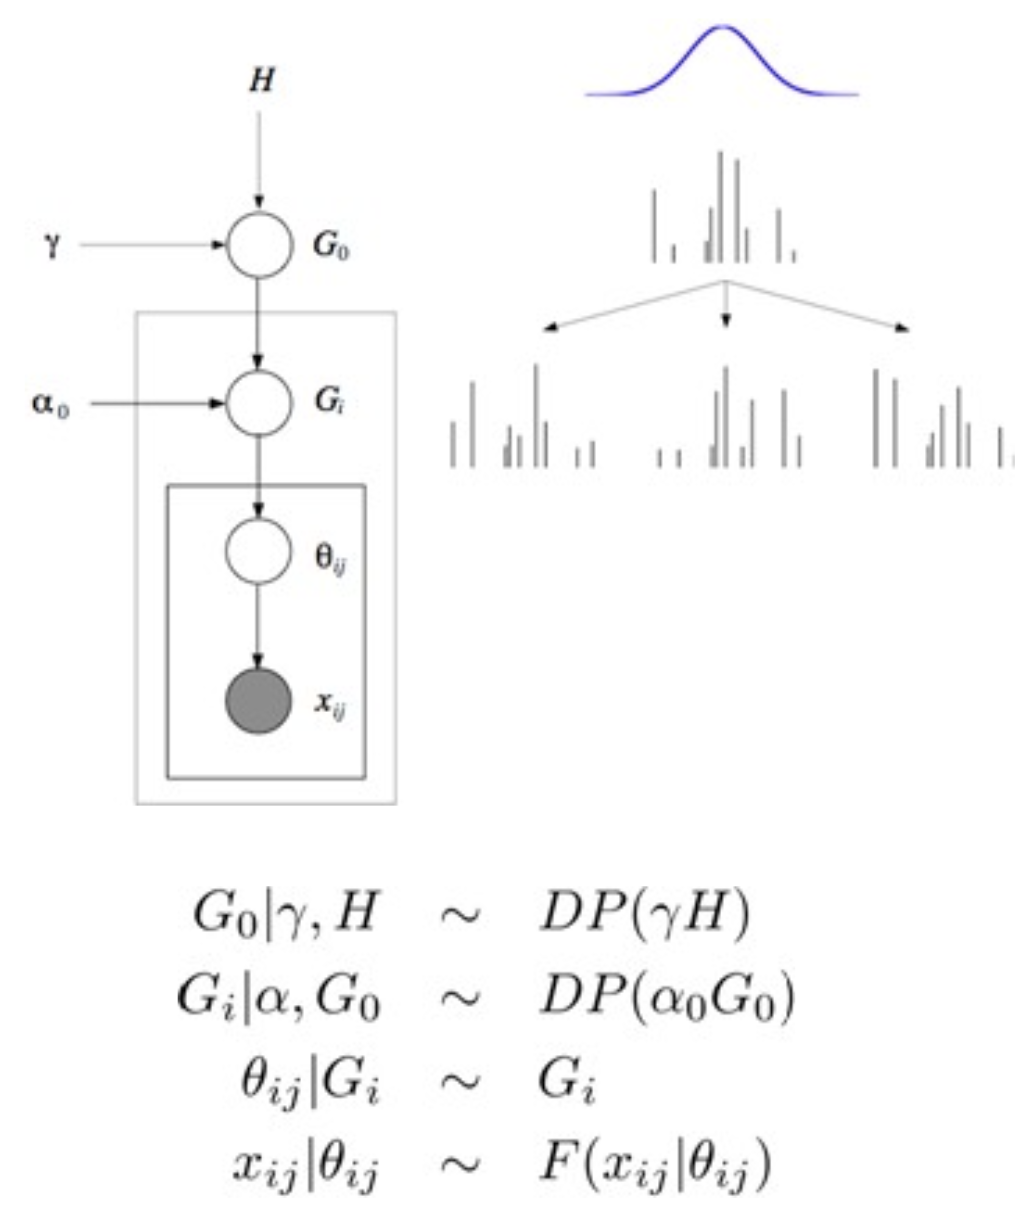
\includegraphics[width=.5\textwidth]{figures_julyan/beyond_DP/HDP}
\end{center}
\hfill\textcolor{gray}{[Image by M. Jordan]}
\pause
	
	Associated partition distr. called \alert{Chinese Restaurant Franchise}.
\end{frame}

\begin{frame}{Indian Buffet process}
	Feature allocation model by  \citet{ghahramani2006infinite}, where observations may share several features.\pause 	\alert{Generative model is as follows}
	\begin{itemize}[<+->]
		\item first customer samples $\text{Poisson}(\gamma)$ dishes
		\item second customer chooses every dish of first customer \textit{wp} $1/2$, plus  $\text{Poisson}(\gamma/2)$ new dishes
		\item $\ldots$
		\item $i$th step: $K$ dishes have been sampled, each by $n_1,\ldots,n_K$ customers;  $i$th customer chooses $j$th dish  \textit{wp} $n_j/i$, plus  $\text{Poisson}(\gamma/i)$ new dishes.
	\end{itemize}\pause
	
	\alert{Log growth}: $K_n\sim \text{Poisson}(\gamma\log n)$.
	
		\begin{center}
			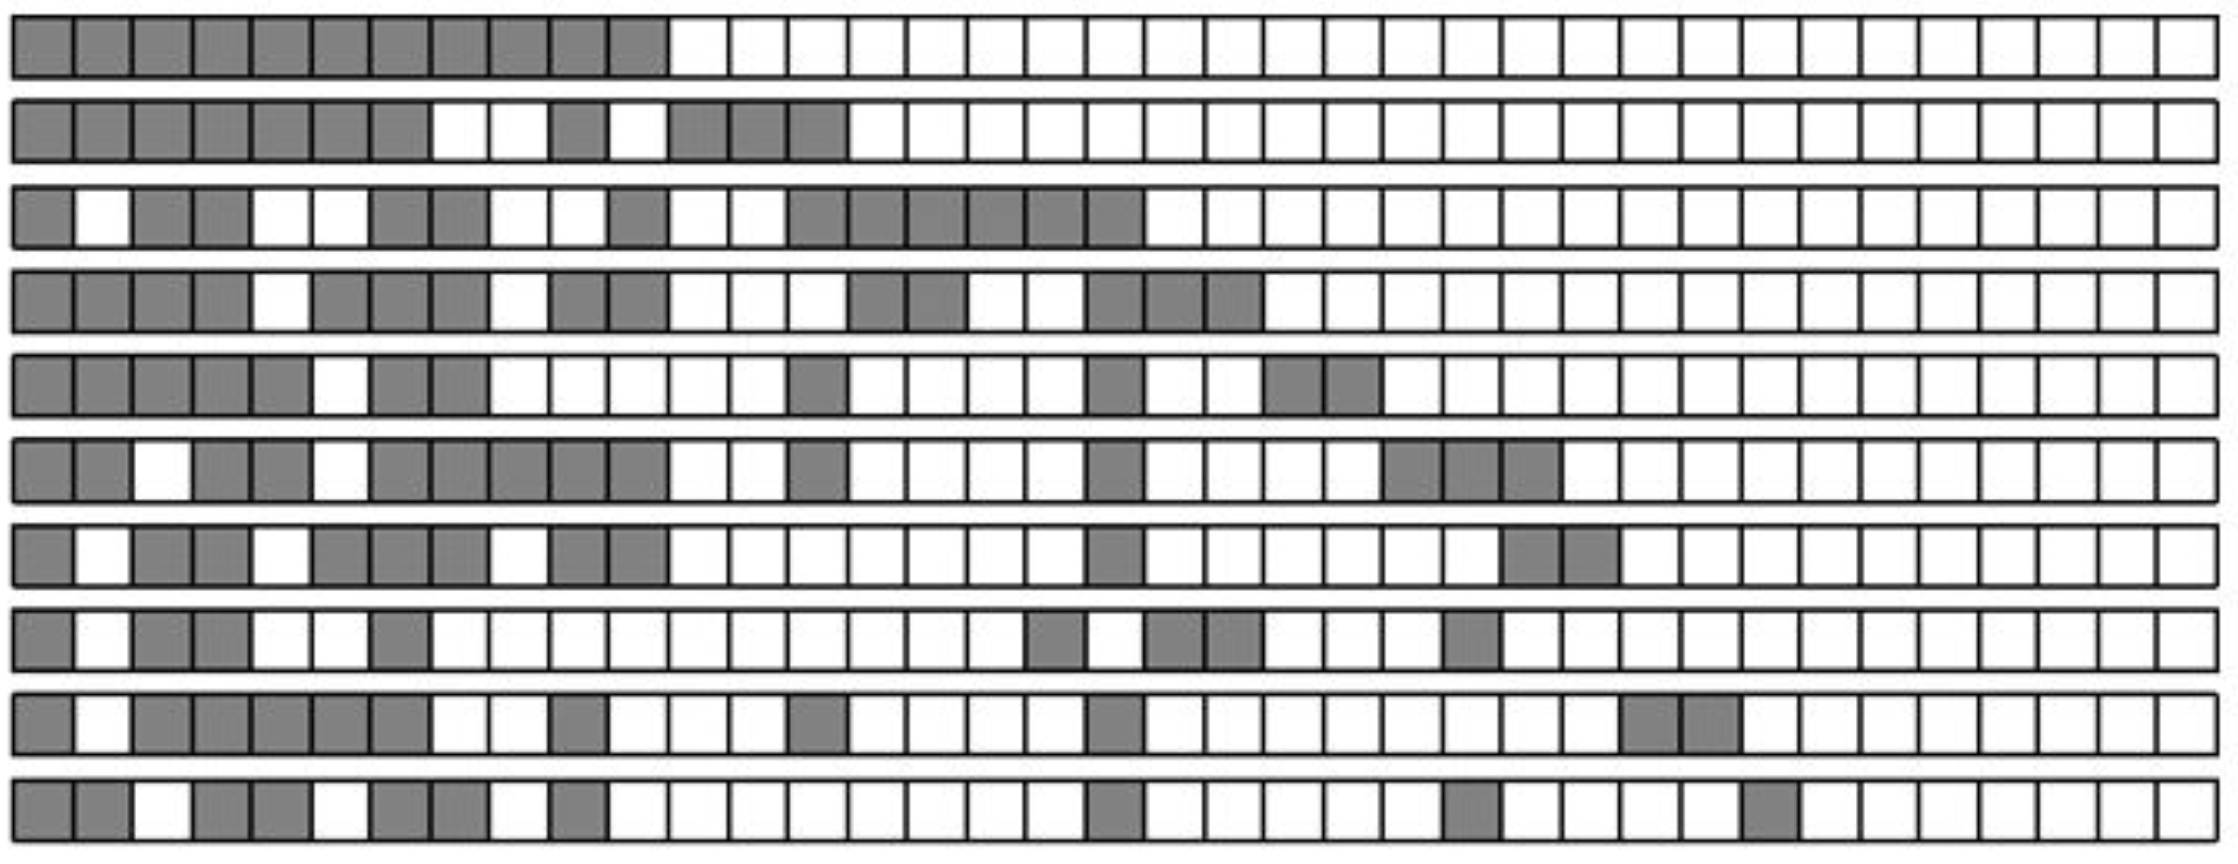
\includegraphics[width=.7\textwidth]{figures_julyan/beyond_DP/IBP_draw}
		\end{center}
		\hfill\textcolor{gray}{[Image by M. Jordan]}
\end{frame}


%
%%%%%%%%%%%%%%%%%%%%%%
\section{Asymptotic evaluation of the posterior}
%%%%%%%%%%%%%%%%%%%%%%

%%%%%%%%%%%%%%%%%%%%%%
\subsection{Introduction}
%%%%%%%%%%%%%%%%%%%%%%

\begin{frame}{What comes to $your$ mind when you hear ``Asymptotics''?}
\end{frame}


\begin{frame}{Why Asymptotics}
\begin{itemize}[<+->]
\item Construction of a prior on a nonparametric space is difficult
\item We cannot hope to cover all the space of density (for example) with our prior (the prior does not have full support)
\item \alert{We need to check that our inference is not completely off! }
\end{itemize}
 \pause 
\begin{block}{Parametric setting}
We have the celebrated \alert{Bernstein-von Mises} theorem that implies that the effect of the prior on the posterior inference vanishes when the amount of information grows. 
\end{block}
\begin{center}
\alert{This is not true anymore in a nonparametric setting! }
\end{center}
\end{frame}

\begin{frame}{Why Asymptotics}
A first order approximation is to consider the asymptotic setting:
\pause
\begin{itemize}[<+->]
\item Adopt a Frequentist point of view: ``There exists a \emph{true} parameter $\theta_0$, and we study the posterior distribution with data generated w.r.t. $\theta_0$.'' 
\item Ideally, the posterior distribution will \alert{concentrate} around $\theta_0$ when $n\to \infty$.
\end{itemize}
\end{frame}



\begin{frame}{References}
\begin{itemize}
	\item \fullcite{Ghosh2003}
	\item \fullcite{hjort2010bayesian}
	\item \fullcite{ghosal2017fundamentals}
\end{itemize}

\end{frame}



\subsection{Posterior consistency}

%\subsection{Some definition}
\begin{frame}{Consistency}
Setting:
\begin{itemize}
\item $\forall n \in \N$, let $\Xn$ be some observations in a sample space $\{\mathcal{X}^n,\mathcal{A}^n\}$ with distribution $P_\theta$
\item $\theta \in \Theta$ with $(\Theta,d)$ a (semi-)metric space 
\end{itemize}
\pause
Let $\Pi$ be a prior distribution on $\Theta$ and $\Pi(\cdot|\Xn)$ a version of its posterior distribution. 
\begin{definition}[Consistency]
The posterior distribution $\Pi(\cdot|\Xn)$ is said to be \alert{weakly consistent} at $\theta_0$ if for all $\epsilon >0$ 
$$
\Pi\left(d(\theta,\theta_0) > \epsilon|\Xn\right) \xrightarrow[n\to \infty]{P_{\theta_0}} 0. 
$$
If the convergence is \alert{almost sure}, then the posterior is said to be \alert{strongly consistent}.
\end{definition}
\end{frame}

%\begin{frame}{Consistency}
%\begin{center}
%\animategraphics[height = 0.8\textheight,autoplay,loop]{10}{figures_julyan/asymp/images/gif_contraction/0000}{01}{99}
%\end{center}
%\end{frame}

%\begin{frame}{Consistency}
%\begin{block}{Other view of consistency}
%\begin{itemize}
%\item Consistency can be summarized by saying that the full posterior distribution converge weakly to a Dirac mass at $\theta_0$ in $P_0$ probability or $P_0$ almost surely. 
%\item Posterior consistency can also be characterized through the posterior distribution of $\psi(\theta)$ for some tests function $\psi \in \Psi$.  
%\end{itemize}
%\end{block}
%\end{frame}

\begin{frame}{Point estimators}
Naturally one will hope that posterior consistency implies that some summary of the posterior location would be a consistent estimator. 
\pause 

\begin{theorem}
Let $\Pi(\cdot|\Xn)$ be a posterior distribution on $\Theta$ and suppose that it is consistent at $\theta_0$ relative to a metric $d$ on $\Theta$. For $\alpha \in (0,1)$, define $\hat{\theta}_n$ as the centre of the smallest ball containing at least $\alpha$ of the posterior mass. Then 
$$
d(\hat{\theta}_n, \theta_0) \xrightarrow[n\to \infty]{P_{\theta_0}, \text{ or } P_{\theta_0}~a.s. } 0. 
$$   
\end{theorem}
\end{frame}


\begin{frame}[allowframebreaks]{Extra notes}
	Take $\alpha = 1/2$ for simplicity and consistency in probability. Define $B(\theta,r)$ the closed ball of radius $r$ centred around $\theta$, and let 
	$$
\hat{r}(\theta) = \inf\{r, \Pi(B(\theta,r) | \Xn)\geq 1/2  \}
	$$
	(and $\inf$ over the empty set is $\infty$). Now let $\hat{\theta}_n$ be such that 
	$$
\hat{r}(\hat{\theta}_n) \leq \inf_{\theta \in \Theta} r(\theta) + 1/n
	$$ 
	Consistency implies that $\Pi(B(\theta_0,\epsilon) |\Xn) \to 1$ so $\hat{r}(\theta_0) \leq \epsilon$ with probability tending to 1. Furthermore, $\hat{r}(\hat{\theta}_n)  \leq \hat{r}(\theta_0) + 1/n $ thus $\hat{r}(\hat{\theta}_n)  \leq \epsilon + 1/n$ with probability tending to $1$.
 
	In addition, $B(\theta_0,\epsilon)\cap B(\hat{\theta}_n,\hat{r}(\hat{\theta}_n)) \neq \emptyset$ otherwise $\Pi(B(\theta_0,\epsilon)\cup B(\hat{\theta}_n,\hat{r}(\hat{\theta}_n)) |\Xn) = \Pi(B(\theta_0,\epsilon)|\Xn) + \Pi(B(\hat{\theta}_n,\hat{r}(\hat{\theta}_n)) |\Xn) \to 1 + 1/2$. So we have 
	$$
d(\theta_0,\hat{\theta}_n) \leq \hat{r}(\hat{\theta}_n) + \epsilon \leq 2\epsilon + 1/n
	$$
	with probability that goes to $1$. 
\end{frame}

\begin{frame}{Point estimator}
\begin{itemize}
\item If $\Theta$ is a vector space, then one might want to use the \alert{posterior mean}.
\item But... weak convergence to a Dirac does not imply convergence of moments.
\item Consistency of the posterior mean requires additional assumptions such as boundedness of posterior moments in probability or a.s. for some $p>1$ would be sufficient. 
\end{itemize}
\end{frame}

\begin{frame}{Point estimator}
% Under some assumption on the space $\Theta$ and on the metric $d$ one can show consistency of the posterior mean through consistency of the posterior distribution. 
\begin{theorem}[Posterior mean]
Assume that the balls of the metric space $(\Theta,d)$ are convex. Suppose that for any sequence $\theta_{1,n}, \theta_{2,n}$ in $\Theta$ and $\lambda_n \to 0$
$$
d(\theta_{1,n}, (1-\lambda_n) \theta_{1,n} + \lambda_n \theta_{2,n}) \to 0 
$$
Then consistency of the posterior distribution implies consistency of the posterior mean. 
\end{theorem}

\end{frame}


\begin{frame}[allowframebreaks]{Extra notes}
	% For $\epsilon >0$ we have 
	% \begin{align*}
	% d(\E(\theta|\Xn),\theta_0) &\leq \E(d(\theta,\theta_0)) \\ 
 % & = \int_{B(\theta_0,\epsilon)} d(\theta,\theta_0) \Pi(d\theta|\Xn) + \int_{B(\theta_0,\epsilon)^c} d(\theta,\theta_0) \Pi(d\theta|\Xn)
	% \end{align*}
	Let $\epsilon >0$ and write $\hat{\theta}_n = \int \theta \Pi(d\theta|\Xn)$. We decompose 
	$$
\hat{\theta}_n = \int_{B(\theta_0,\epsilon)} \theta \Pi(d\theta|\Xn) + \int_{B(\theta_0,\epsilon)^c} \theta \Pi(d\theta|\Xn) = \theta_{1,n} (1-\lambda_n) + \lambda_n\theta_{2,n}
	$$
	where $\theta_{1,n} =\int_{B(\theta_0,\epsilon)} \theta \frac{\Pi(d\theta|\Xn))}{\Pi(B(\theta_0,\epsilon)|\Xn)} $, $\lambda_n = \Pi(B(\theta_0,\epsilon)|\Xn)$ and similarly for $\theta_{2,n}$ on the complement of $B(\theta_0,\epsilon)$.
	Using Jensen inequality we have 
	\begin{equation*}
	d(\theta_{n,1},\theta_0) \leq \int_{B(\theta_0,\epsilon)} d(\theta,\theta_0) \frac{\Pi(d\theta|\Xn))}{\Pi(B(\theta_0,\epsilon)|\Xn)} \leq \epsilon
	\end{equation*}
	In addition we have 
	$$
	d(\hat{\theta}_n,\theta_0) \leq d(\theta_{n,1},\theta_0) + d(\theta_{n,1}, \theta_{1,n} (1-\lambda_n) + \lambda_n\theta_{2,n} ).
	$$
	Using the fact that $\lambda_n \to 0$ since the posterior is consistent, we have the desired result. 
	\begin{remark}
	For the condition on $d$ to hold, one can assume it to be convex and uniformly bounded. 
	\end{remark}
\end{frame}

\begin{frame}{A first consistent posterior}
\begin{example}[Dirichlet process]
Assume the following model 
\begin{align*}
X_1, \dots, X_n &\overset{iid}{\sim} P, \\ P &\sim \text{DP}(M\alpha)
\end{align*}
Consider the semi-metric $d_A(P,Q) = |P(A) - Q(A)|$ for some measurable event $A$ on $\Theta$, then $\Pi(\cdot |\Xn)$ is \alert{strongly consistent} at any $P_0$ for $d_A$. 
\end{example}
\pause 

From this result, we can easily obtain consistency under the weak topology. We could also obtain stronger consistency using Glivenko--Cantelli theorem. 
\end{frame}


\begin{frame}[allowframebreaks]{Extra notes}
	Consider $\Pi(|P(A) - P_0(A)| \geq \epsilon | \Xn)$ which calls for applying Markov inequality. Properties of the Dirichlet process imply that $$P\vert \Xn \sim \text{DP}(M\alpha + n\mathbb{P}_n),$$ thus $$P(A)\vert \Xn \sim \text{Beta}(M\alpha(A) + n\mathbb{P}_n(A), M\alpha(A^c) + n\mathbb{P}_n(A^c)).$$ We thus have 
	\begin{align*}
	\E(P(A)|\Xn) &= \frac{M}{M+n} \alpha(A) + \frac{n}{M+n} \mathbb{P}_n(A) := \bar{P}(A)\\
    \mathrm{var}(P(A)|\Xn) &= \frac{\bar{P}(A)\bar{P}(A^c)}{1 + n + M} \leq \frac{1}{4(1+n+M)}.
	\end{align*}
Markov inequality gives 
	\begin{align*}
	\Pi(|P(A) - P_0(A)| \geq \epsilon | \Xn) &\leq \frac{1}{\epsilon^2} \left( |\bar{P}(A) - P_0(A)|^2 +  \mathrm{var}(P(A)|\Xn) \right)\\
	 & \to 0 ~ [P_0, a.s. ] 
	\end{align*}
using the law of large numbers on $\mathbb{P}(A)$.
\end{frame}
%\subsection{Why bother?} 

\begin{frame}{Bayesian modelling perspective}
From a Bayesian point of view, a \alert{Dirac measure at $\theta_0$} corresponds to perfect knowledge of the parameter. 
\begin{itemize}
	\item Prior and posterior distributions model our knowledge about the parameter.
	\item Consistency thus implies that when the amount of information grows, we tend towards perfect knowledge of the parameter. 
\end{itemize}
\end{frame}

\begin{frame}{A validation of Bayesian methods}

The frequentist setting where there exists a \emph{true} parameter $\theta_0$ that generates the data can be seen as an idealized set-up. 
\begin{itemize}
	\item An experimenter feeds a Bayesian with some data using the same data-generating mechanism. 
	\item When the number of observation grows, a Bayesian should be able to pin-point the data-generating mechanism, whatever their prior. 
	\item<2> \alert{A prior that does not lead to a consistent posterior should not be used.} 
\end{itemize}

\end{frame}

\begin{frame}{Robustness}

Two Bayesians walk into a bar... with \emph{almost} the same prior, then their posterior inference should not differ that much. \pause 
\begin{itemize}
\item Let $\Pi_1$ be the prior of Bayesian number 1
\item Bayesian number 2 uses an ``$\epsilon$-corrupted'' prior $\Pi_2 = (1-\epsilon)\Pi_1 + \epsilon \delta_{p_0}$ for some $p_0 \in \Theta$
\end{itemize}
The posterior of Bayesian number 2 is consistent at $p_0$ (to be seen later), now what if $\Pi_1$ is not consistent at $p_0$? 
\pause 
Let $d_W$ be the metric for the weak topology, then $d_W(\Pi_1(\cdot|\Xn), \Pi_2(\cdot|\Xn))$ would not go to $0$. 

\end{frame}


\begin{frame}[allowframebreaks]{Extra notes}
There exists some $\varepsilon_0 >0$ such that 
$$
\Pi_{n,1}(B(\theta_0,\varepsilon_0)|\Xn) \not\to 0 
$$
Thus 
$$
|\Pi_{n,1}(B(\theta_0,\varepsilon_0)|\Xn) - \Pi_{n,2}(B(\theta_0,\varepsilon_0)|\Xn) | \not\to 0
$$
since $\Pi_{n,2}(B(\theta_0,\varepsilon_0)|\Xn) \to 0$.
\end{frame}

\subsubsection{Doob's Theorem}


\begin{frame}{Doob's Theorem}
Can one get general conditions on the prior to ensure that it is consistent? \pause 
\begin{itemize}[<+->]
 \item A first answer: Doob's Theorem
 \item The posterior is consistent at every $\theta$ $\Pi$-a.s. 
 \end{itemize} 
 \pause 
 Consider the case of \emph{i.i.d.} observations
 \begin{theorem}[Doob's Theorem]
 Let $\{\mathcal{X}^n, P_\theta, \Theta\}$ be a statistical model where $\{\mathcal{X}^n,\mathcal{A}^n\}$ is a Polish space with Borel $\sigma$-field and $\Theta$ a Borel subset of a Polish space. Suppose that the map $\theta \mapsto P_\theta(A)$ is Borel measurable for evey $A\in \mathcal{A}$ and $\theta \mapsto P_\theta$ is one-to-one. \\
 Then for any prior distribution $\Pi$ on $\Theta$, if $X_1, \dots, X_n \overset{iid}{\sim} P_\theta$, $\theta \sim \Pi$, \alert{the posterior is strongly consistent at any $\theta$ $\Pi$-a.s.}
 \end{theorem}
\end{frame}

\begin{frame}{Doob's Theorem}
\begin{block}{Some remarks on Doob's Theorem}
\begin{itemize}[<+->]
\item The conditions of the theorem are extremely weak
\item And no conditions on the prior
\item However this is only true \alert{$\Pi$-almost surely}. 
\item Note: the $\Pi$-null set can be quite big! we can be happy with this result only if we are confident that the parameters are on the support of the prior. In general no one can be sure that the parameter generating the data inside the support of the prior, this is a real problem in fact in general the support of the prior can be quite thin. 

An extreme example is the case were the prior is a Dirac on some parameter $\theta_0$. Then Doob's theorem still holds. 

%An exception is the case where $\Theta$ is countable. 
\end{itemize}
\end{block}
\end{frame}

\subsubsection{Schwartz approach}

%\paragraph{Setting}

\begin{frame}{Setting}
Doob's approach is not enough to show consistency of the posterior. For simplicity we focus on the \textcolor{forestgreen}{density estimation} setting.
\begin{itemize}
 \item $\Theta$ is the set of probability density functions on $\mathcal{X}$ w.r.t. a common dominating measure $\nu$. We denote the parameter $p$ (instead of $\theta$) and $P$ the associated probability measure. 
 \item Observations follow $X_1, \dots, X_n \overset{iid}{\sim} p$, and $p\sim \Pi$.
 \end{itemize}
\pause 

Considering  \textcolor{forestgreen}{density estimation} makes things easier  without being too simplistic. The same results can be extended to  \textcolor{forestgreen}{nonparametric regression}.  
\end{frame}

%\paragraph{Hypotheses}

\begin{frame}{KL property}
To achieve consistency, we do not want to require that the true parameter $p_0$ is  \textcolor{orange2}{inside} the support of $\Pi$. However we still require \textcolor{orange2}{some prior mass \emph{near} $p_0$}. 
\begin{definition}[Kullback--Leibler]
Let $p$ and $p_0$ be two p.d.f. with respect to a common measure such that $p_0 \ll p$. Then the Kullback--Leibler divergence between $p$ and $p_0$ is 
$$
\text{KL}(p,p_0) = \int p_0 \log(p_0/p) d\nu.
$$ 
\end{definition}

\end{frame}

\begin{frame}{KL property}
\begin{definition}[KL property]
We say that a prior distribution $\Pi$ satisfies the \textcolor{orange2}{Kullback--Leibler property} at $p_0$ if for every $\epsilon>0$, 
$$
\Pi(p:\,\text{KL}(p,p_0)\geq \epsilon) >0 
$$
We note $p_0\in \text{KL}(\Pi)$ and alternatively will say that $p_0$ is in the KL-support of $\Pi$.
\end{definition}
\pause
This extends quite a lot the parameters at which the posterior can be consistent. 
\end{frame}


\begin{frame}{Existence of tests}

The other requirement is that the parameter set is not too complex.   

\begin{definition}[Exponentially consistent tests]
We say that a sequence of tests $\phi_n$ for $H_0: p = p_0$ versus $H_1: p \in U^c$ is exponentially consistent if 
$$
P_0^n(\phi_n) \lesssim e^{-Cn}, ~ \sup_{p\in U^c} P^n(1-\phi_n) \lesssim e^{-Cn} 
$$
\end{definition}
A test is understood as a measurable map $\mathcal{X}^n \to [0,1]$ and the corresponding statistic $\phi_n(X_1, \dots, X_n)$. $\phi_n$ is interpreted as the probability that the null is rejected. 
\end{frame}


\begin{frame}[allowframebreaks]{Extra notes}
	The existence of tests means that we can differentiate between $p_0$ and parameter in $U^c$. 

	It is enough to have uniformly consistent sequence of test 
	$$
P_0(\phi_n) \to 0, ~ \sup_{p\in U^c} P(1-\phi_n) \to 0. 
	$$

Since the test is uniformly consistent then there exists $k\in \N$ such that $P_0^k(\phi_k) \leq 1/4$, $P^k(1-\phi_k) \leq 1/4$. Now for $n$ large, write $n = mk+r$. Slice $\Xn = (X_1, \dots, X_n)$ into $m$ sub-sample of size $k$ $\Xn_l = (X_{(l-1)k+1},\dots, X_{lk})$ and define $Y_{l,n} = \phi_k(\Xn_l)$. Now create a new test $\psi_n = \I\{\bar{Y}_m > 1/2\}$. We have for every $p \in U^c$, $P(1-Y_j) \leq 1/4$
\begin{multline*}
P(\psi_n) = P(\bar{Y} \leq 1/2) = P(1-\bar{Y} \geq 1/2) = \\ 
P(1-\bar(Y) \geq 1/2) \leq e^{-2m/16} \lesssim e^{-Cn}
\end{multline*}
Using Hoeffding inequality: $\P(\bar{X} - \E(X) \geq \epsilon ) \leq \exp\left\{ - 2 \epsilon^2 m \right\}$.
\end{frame}


%\paragraph{Schwartz Theorem}

\begin{frame}{Schwartz Theorem}
\begin{theorem}
Let $\Pi$ be a prior distribution on $\Theta$ such that $p_0\in KL(\Pi)$. Let $U$ be a neighbourhood of $p_0$ such that there exists an exponentially consistent sequence of tests for $p_0$ against $U^c$. Then 
$$
\Pi(U^c | \Xn) \to 0 ~ [P_0 a.s].
$$
\end{theorem}\pause

This theorem is not due to Herman Schwarz (without t!), nor to Laurent Schwartz the Fields Medalist! But to Lorraine Schwartz, former student of Lucien Le Cam.
\end{frame}


\begin{frame}[allowframebreaks]{Extra notes} 
$$
\Pi(U^c|\Xn) = {\int_{U^c} \prod_{i=1}^n  \frac{p}{p_0}(X_i) d\Pi(p) \over \int_{\mathcal{P}} \prod_{i=1}^n  \frac{p}{p_0}(X_i) d\Pi(p)} := \frac{N_n}{D_n}.
$$
We first show $\lim\inf D_n e^{n\epsilon} / \Pi(KL(p,p_0)>\epsilon)   \geq 1 $, $P_0[a.s.]$. Let $\Pi_0(\cdot) = \Pi(\cdot \cap \text{KL}(p,p_0)>\epsilon)/\Pi(KL(p,p_0)>\epsilon)$. Then 
\begin{align*}
\log(D_n) &\geq \log\left(\int_{KL(p,p_0)>\epsilon} \frac{p}{p_0}(X_i) d\Pi_0(p)\right) + \log(\Pi(KL(p,p_0)<\epsilon)) \\ 
&\geq \int_{KL(p,p_0)>\epsilon} \log\left( \prod_{i=1}^n  \frac{p}{p_0}(X_i) \right) d\Pi_0(p) + \log(\Pi(KL(p,p_0)<\epsilon)) \\ 
&=  \sum_{i=1}^n \int \log \frac{p}{p_0}(X_i) d\Pi_0(p) + \log(\Pi(KL(p,p_0)<\epsilon)) 
\end{align*}
The law of large numbers implies 
$$
\frac{1}{n} \sum_{i=1}^n \int \log \frac{p}{p_0}(X_i) d\Pi_0(p) \to P_0 \int \frac{p}{p_0}(X_i) d\Pi_0(p),~ P_0[a.s.] 
$$
which is $- \int \text{KL}(p,p_0) d\Pi_0(p) > -\epsilon $.
Thus 
$$
\lim\inf D_n e^{n\epsilon} / \Pi(KL(p,p_0)>\epsilon)   \geq 1 ,~ P_0[a.s.]
$$ 
	For $n$ large enough we have the following $P_0[a.s.]$ 
	\begin{align*}
	\Pi(U^c|\Xn) & \leq  \phi_n + (1-\phi_n) \frac{N_n}{D_n} \\
                 & \leq \phi_n  + (1-\phi_n) N_n e^{\epsilon n } \Pi(KL(p,p_0)>\epsilon)  
	\end{align*}
Furthermore we have that 
\begin{align*}
P_0^n  N_n (1-\phi_n) &= P_0^n  \int_{U^c} (1-\phi_n) \prod_{i=1}^{n} \frac{p}{p_0}(X_i) \Pi(dp) \\ 
                      &= \int_{U^c} P^n (1-\phi_n) \Pi(dp) \leq e^{-Cn} 
\end{align*}

We thus get $P_0\Pi(U^c|\Xn) \leq e^{-C'n}$ for $\epsilon < C$ and for $C' = C - \epsilon$. Using Borel--Cantelli we get that $\Pi(U^c |\Xn) \to 0 P_0[a.s.]$. 
\end{frame}

\begin{frame}{Schwartz Theorem}
% In this original version of Schwartz theorem, we need to be able to test away for all the function in $U^c$. This might not be possible for strong metrics such as $L_1$ metrics. 
\begin{itemize}
\item Need to test away all densities in $U^c$
\item Might not be possible for strong neighbourhood of $p_0$ ($L_1$ metrics)
\end{itemize}
\pause 
\begin{block}{Extension of Schwartz theorem}
The idea is that not \emph{all} functions in $U^c$ matters and we can discard function with very low prior probabilities. 
\end{block}
\pause 
\begin{theorem}
The results of the previous theorem are still valid if we replace the assumption on the existence of tests by: 
\begin{align*}
&\Theta_n \subset \Theta \\ 
&\Pi(\Theta_n) \leq e^{-Cn}, ~ P_0^n \phi_n \leq e^{-Cn}, ~ \sup_{p \in U^c \cap \Theta_n} P(1-\phi_n) \leq e^{-Cn} 
\end{align*}
\end{theorem}
\end{frame}

%\paragraph{Existence of tests}

\begin{frame}{Existence of tests}

Schwartz' theorem requires the existence of exponentially consistent tests.
\begin{itemize}[<+->]
\item We can differentiate between $\theta_0$ and $U^c$
\item The model is not too complex 
\end{itemize}
\pause 
\begin{block}{Question}
When do such tests exist? 
\end{block}

Let's see the example of iid observations. 
\end{frame}


\begin{frame}{Sketch of the proof}

\begin{itemize}[<+-|alert@+>]
\item Cannot directly construct test against $U^c = \{p, d(p,p_0) > \epsilon \}$... 
\item Construct an exponentially consistent test against a generic ball that is at least at distance $\epsilon$
\item Cover $U^c$ with $N$ of these balls, and construct a test from the $N$ corresponding tests.
\end{itemize}

\end{frame}


%\paragraph{Consistency under Entropy bound}

\begin{frame}{Consistency under Entropy bound}
We combine the preceding results to get general conditions \alert<2->{on the prior} and \alert<2->{on the model}, that ensure consistency. 
\begin{overprint}
\onslide<3>{
	\begin{theorem}
	The posterior is strongly consistent relative to the $L_1$ distance at every $p_0$ in the KL-support of the prior if for every $\epsilon>0$ there exist $\Theta_n$ such that for $C>0$ and $0<c < 1/2$
	$$
\Pi(\Theta_n^c) \leq e^{-Cn},~ \log N(\epsilon,\Theta_n,\Vert\cdot\Vert_1) \leq c n \epsilon_n^2,
	$$
	for $n$ large enough. 
	\end{theorem}

}
\end{overprint}

\end{frame}



%%%%%%%%%%%%%%%%%%%%%%%%%%%%%%%%%%%%%%%%%%%%%%%%%%%%%%
\subsection{Concentration rates}
%%%%%%%%%%%%%%%%%%%%%%%%%%%%%%%%%%%%%%%%%%%%%%%%%%%%%%


\begin{frame}{Definition}

Contraction rates are a refinement of posterior consistency. \pause 
\begin{itemize}[<+-|alert@+>]
\item How fast posterior concentrates its mass around the true parameter
\item Helps to see how much the prior influences the posterior
\end{itemize}
\pause 

\begin{definition}
Let $\epsilon_n$ be a positive sequence. The posterior contracts at the rate $\epsilon_n$ at $\theta_0$ if for any $M_n \to \infty$ 
$$
\Pi(d(\theta,\theta_0)> M_n \epsilon_n|\Xn) \xrightarrow[n \to \infty]{P_{\theta_0}} 0 
$$
If all the experiments share the same probability space and the convergence is $P_{\theta_0}[a.s]$ we say that the posterior contracts in the strong sense.
\end{definition}

\end{frame}


\begin{frame}{Remarks}

\begin{itemize}[<+->]
\item Any slower rate than $\epsilon_n$ also fits the definition so we will say \emph{a} posterior contraction rate
\item We will naturally try to find the fastest possible rate! 
\end{itemize}
\pause 
\begin{block}{Regarding $M_n$}
\begin{itemize}[<+->]
\item The sequence $M_n$ plays	 virtually no role in the posterior rate. In many cases it can be fixed to a constant $M$. 
\item For finite dimensional models $M_n$ must be allowed to grow to obtain the usual $n^{-1/2}$ rate in smooth models. 
\end{itemize}

\end{block}


\end{frame}


\begin{frame}{Consequences of posterior contraction}
\begin{block}{Point Estimator}
\begin{itemize}[<+->]
\item Let $\hat{\theta}_n$ = centre of the smallest ball that contains at least $1/2$ of the posterior mass. 
\item Assume that the posterior contracts at $\theta_0$ with rate $\epsilon_n$ for the metric $d$
\end{itemize}
\pause
Then $d(\hat{\theta}_n,\theta) = O_P(\epsilon_n)$ in $P_0$ probability (or a.s. if strong contraction).
\end{block}
\end{frame}

\begin{frame}{Consequences of posterior contraction}

\begin{block}{Posterior mean}
If the metric $d$ is bounded and $\theta \mapsto d^s(\theta, \theta_0)$ is convex for some $s \geq 1$ then the posterior mean $\tilde{\theta}_n$ satisfies 
$$
d(\tilde{\theta}_n,\theta_0) \leq M_n\epsilon_n + \Vert d \Vert_\infty^{1/s} \Pi_n(d(\theta,\theta_0) \geq M_n \epsilon_n|\Xn)^{1/s}.
$$
\end{block}
\pause 
\begin{itemize}
\item First term is the dominating term
\item The second term is exponentially small in general
\end{itemize}
\end{frame}

\begin{frame}{Some first Examples - Parametric models}
\begin{itemize}[<+->]
\item Let $X_1, \dots, X_n |\theta \overset{iid}{\sim} \mathcal{B}(\theta) $, and $\theta\sim \text{Beta}(\alpha,\beta)$. The posterior contracts at a rate $n^{-1/2}$
\item Let $X_1,\dots, X_n|\theta \overset{iid}{\sim} \mathcal{U}([0,\theta])$ and $\pi(\theta) \propto \theta^{-a}$. The posterior contracts at a rate $n^{-1}$.
\end{itemize}
\pause 
\begin{block}{Parametric regular models}
In fact for all regular finite dimensional models the \alert{Bernstein von-Mises} theorem implies a posterior rate of $n^{-1/2}$. 
\end{block}
\end{frame}

\begin{frame}{Nonparametric example: Dirichlet Process}

\begin{itemize}
\item $X_1, \dots, X_n | P \overset{iid}{\sim} P $ 
\item $P\sim \text{DP}(M\alpha)$ for $\alpha$ a probability measure on $\mathcal{X}$. 
\end{itemize}

The posterior distribution is $P|\Xn \sim \text{DP}(M\alpha + n\mathbb{P}_n)$. 
\pause 
\begin{block}{Local semi-metric\footnote{ie $d(P,Q) \geq 0$ but might be 0 for $P\neq Q$.}}
For a measurable set $A$, let $d(P,Q) = |P(A) - Q(A)|$. The posterior distribution is consistent at $P_0$ at a rate $n^{-1/2}$.  
\end{block}
\pause 

\begin{block}{Global metric}
For $\nu$ a $\sigma$-finite measure and $F$ and $G$ two c.d.f. let $d(F,G) = \Vert F-G\Vert_\nu^2 = \int (F(t) - G(t))^2 d\nu(t)$. The posterior contracts at rate $n^{-1/2}$ at $P_0$ for this metric. 
\end{block}

\end{frame}


\begin{frame}{Nonparametric example: White Noise}
Consider the following model for $W_t$ a white noise
$$
X_t = f(t) + n^{-1/2}W_t.
$$
Projecting this model onto the Fourier basis if $f\in L_2$, we have the equivalent formulation
$$
X_{i,n} = \theta_i + n^{-1/2} \epsilon_i,~ i \in \N^* 
$$
$\theta \in \ell_2(\R)$. Assume the following prior 
$$
\theta_i \overset{ind.}{\sim} \mathcal{N}(0, i^{-2\alpha - 1}).  
$$ 
If $\theta_0 \in \mathcal{S}_\beta^{2,2}$ then the posterior contracts at $\theta_0$ at the rate $n^{-\min(\alpha,\beta)/(2\alpha + 1)}$. 
\end{frame}

\subsubsection[iid case]{General theorem in the iid case}


%\subsection{First Theorem}

\begin{frame}{General theorem}
\begin{itemize}[<+->]
\item Result similar to Schwartz theorem? 
\item We focus on the case of i.i.d observations $X_1, \dots, X_n \overset{iid}{\sim} P$ 
\item The parameter set $\Theta$ is the set of probability densities with respect to a common dominating measure $\mu$. 
\end{itemize}
\pause 

Let $\Pi_n$ be a sequence of priors. We study the sequence of posterior distributions $\Pi_n(\cdot|\Xn)$ under the assumption that the data are generated from $P$. 

\end{frame}


\begin{frame}{General Theorem}
We follow the same steps as for Schwartz' Theorem: 
\begin{itemize}
\item Existence of tests to separate $p_0$ from the complement of balls
\item KL condition: the prior puts enough mass on neighbourhood of $p_0$
\end{itemize}
Define $V_{2,0}$, the 2nd KL variation
$$
V_{2} = P_0 \left( \log^2\left(\frac{p_0}{p}(X) \right)\right),
$$ 
and define two KL neighbourhoods as
\begin{align*}
B_0(p_0,\epsilon) &= \{p, \text{KL}(p_0,p) \leq \epsilon^2\},\\
B_2(p_0,\epsilon) &= \{p, \text{KL}(p_0,p) \leq \epsilon^2, V_{2}(p_0,p) \leq \epsilon^2\}.
\end{align*}

\end{frame}

\begin{frame}{General theorem}

\begin{theorem}[Ghosal, Ghosh and van der Vaart]
Let $d \leq h$ be a metric on $\Theta$ for which balls are convex, and let $\Theta_n \subset \Theta $. The posterior contracts at a rate $\epsilon_n$ for all $\epsilon_n$ such that $n\epsilon_n^2 \to \infty$ and such that for positive constants $c_1$, $c_2$ and any $\underline{\epsilon}_n \leq \epsilon_n$
\begin{align*}
\log N(\epsilon_n, \Theta_n, d) \leq c_1 n \epsilon_n^2, \\ 
\Pi_n(B_{2,0}(p_0,\underline{\epsilon}_n^2)) \geq e^{-c_2 n \underline{\epsilon}_n^2}\\
\Pi(\Theta_n^c) \leq e^{-(c_2+3)n \underline{\epsilon}_n^2}
\end{align*}
\end{theorem}

\end{frame}


\begin{frame}{General Theorem}
\begin{itemize}[<+->]
\item The KL condition can be refined, but the idea is basically the same
\item Entropy condition is useful for the existence of tests
\item Entropy condition can be replaced by a local entropy, which is more like a \emph{dimension of $\Theta_n$}
\end{itemize}
\pause 
\begin{block}{Interpretation}
Assume that $d$ and $KL$ are equivalent
\begin{itemize}[<+->]
\item We need $e^{n\epsilon_n^2}$ balls to cover $\Theta_n$. 
\item If the prior spread evenly the mass on these balls, we have $e^{-Cn\epsilon_n^2}$ mass on each of these balls thus KL condition is satisfied
\item If the spread is uneven, then KL condition might not be satisfied for some $p_0$. 
\end{itemize}
\end{block}
\end{frame}




\subsubsection[Non iid case]{Non iid  observations}




%\paragraph{General result}


\begin{frame}{General observations}

\begin{itemize}[<+->]
\item The previous theorem can be generalized to other models (like regression for instance)
\item But we have to be careful with the metric we use, and the existence of test is not guaranteed! 
\item To be general we will have to assume that we can test away parameters
\end{itemize}
\pause 
\begin{block}{Existence of tests}
Let $d_n$ and $e_n$ be two semi-metrics on $\Theta$. For $\epsilon >0$, and for all $\theta_1 \in \Theta$ such that \alert<6->{$d_n(\theta_0,\theta_1)> \epsilon$} there exists $\phi_n$ 
$$
P_{\Theta_0}^n  \phi_n \leq e^{-Kn\epsilon^2}, ~ \sup_{\theta, \alert<6->{e_n(\theta,\theta_1)\leq \xi \epsilon}} P_{\theta}^n (1-\phi_n) \leq e^{-Kn\epsilon^2}
$$
\end{block}

\end{frame}

\begin{frame}{General theorem}
Define the following KL-neighbourhood 
\begin{align*}
V_{k,0}(f,g) = \int f|\log(f/g) - \text{KL}(f,g)|^k d\mu \\ 
B_n(\theta_0,\epsilon,k) = \left\{ \theta \in \Theta \text{KL}(p^n_{\theta_0},p^n_\theta)\leq n\epsilon^2, V_{k,0}(p_{\theta_0}^n, p^n_\theta) \leq n^{k/2}\epsilon^k \right\}
\end{align*}

\end{frame}
\begin{frame}{General theorem}
\begin{theorem}
Let $d_n$ and $e_n$ be two semi-metrics on $\Theta$, such that tests exists, $\epsilon_n\to 0 $, $n\epsilon_n^2 \to \infty$, $k>1$, $\Theta_n \subset \Theta$ such that for sufficiently large $j\in \N$ 
\begin{align*}
\sup_{\epsilon \geq \epsilon_n} \log N\left( \frac{1}{2} \xi \epsilon, \{\theta \in \Theta_n d_n(\theta_0,\theta)\leq \epsilon \}, e_n  \right) &\leq n\epsilon_n^2\\ 
{\Pi_n(\theta \in \Theta_n, j\epsilon_n \leq d_n(\theta,\theta_0)\leq 2j\epsilon_n) \over \Pi_n(B_n(\theta_0,\epsilon_n,k))} &\leq e^{Kn\epsilon_n^2j^2/2}\\ 
{\Pi_n(\Theta_n^c) \over \Pi_n(B_n(\theta_0,\epsilon_n,k))} & \leq e^{-2n\epsilon_n}
\end{align*}
then $P_{\theta_0}^n \Pi_n(d_n(\theta_0,\theta)\geq M_n \epsilon_n) = o(1)$
\end{theorem}
\end{frame}

%\paragraph{Independent Observations}

\begin{frame}{Independent observations}

\begin{itemize}[<+->]
\item Assume that the measure $P_\theta^n = \bigotimes_{i=1}^{n} P_{i,\theta}$ on some product space $\bigotimes_{i=1}^n \{\mathcal{X}_i, \mathcal{A}_i\}$. 
\item Assume that each measures $P_{i,\theta}$ are absolutely continuous w.r.t $\mu_i$ 
\item Define the Root average Hellinger distance 
$$
d_{n,H} (\theta, \theta') = \left( \frac{1}{n} \sum_{i=1}^n \int (\sqrt{dP_{i,\theta}} - \sqrt{dP_{i,\theta'}})^2 \right)^{1/2}
$$
\end{itemize}
\pause
\begin{lemma}
For all here exists tests $\phi_n$ such that 
$$
P_{\theta_0}^n \phi_n \leq e^{-nd_{n,H}(\theta_0,\theta_1)},~  P_{\theta}^n \leq e^{-nd_{n,H}(\theta_0,\theta_1)}
$$
for all $\theta$ such that $d_{n,H}(\theta,\theta_1) \leq \tfrac{1}{18} d_{n,H}(\theta_0,\theta_1)$
\end{lemma}

\end{frame}


\begin{frame}{Independent observations}
We can also simplify the KL condition in this case. \pause Note that 
$$
KL(p^n_{\theta_0}),p^n_{\theta}) = \sum_{i=1}^n \text{KL}(p_{i,\theta_0},p_{i,\theta})
$$ 
\pause
Furthermore for the KL-variation term we have that 
$$
V_{k,0}(p^n_{\theta_0},p^n_\theta) \leq n^{k/2} C_k \frac{1}{n}\sum_{i=1}^n V_{k,0}(p_{i,\theta_0},p_{i,\theta}) 
$$
\pause
Thus the KL condition can be re-written
\begin{multline*}
B_n^*(\theta_0,\epsilon,k) = \Big\{\theta ,\frac{1}{n} \sum_{i=1}^n \text{KL}(p_{i,\theta_0},p_{i,\theta}) \leq \epsilon^2 , \frac{1}{n} \sum_{i=1}^n V_{k,0}(p_{i,\theta_0},p_{i,\theta})  \leq C_k \epsilon^2 \Big\}
\end{multline*}


\end{frame}

%\paragraph{Example: Nonparametric Regression using Splines}


% \section{Examples}

% \begin{frame}
% \begin{columns}
% \begin{column}{0.5\textwidth}
% \tableofcontents[currentsection]
% \end{column}

% \begin{column}{0.5\textwidth}
% \includegraphics[width = \textwidth]{images/thinker.jpg}
% \end{column}

% \end{columns}

% \end{frame}

\begin{frame}{NP Regression with splines}
Consider the model 
$$
X_i = f(z_i) + \epsilon_i, ~ i=1, \dots, n
$$
where $\epsilon_i \overset{iid}{\sim} \mathcal{N}(0,\sigma^2)$ and the $z_i\in \R$ are known fixed covariates. For simplicity $\sigma^2$ is also assume to be known. \pause 
Let $\mathbb{P}_n^z = \frac{1}{n} \sum_{i=1}^n \delta_{z_i}$ and $\Vert \cdot \Vert_n$ the $L_2(\mathbb{P}_n^z)$ norm
\pause

\begin{lemma}
We have the following results
\begin{align*}
KL(P_{f,i},P_{g,i}) &= \frac{1}{2\sigma^2} (f(z_i) - g(z_i))^2 \\ 
 V_{0,2}(P_{f,i},P_{g,i}) &=\frac{1}{\sigma^2} (f(z_i) - g(z_i))^2 
\end{align*}
\end{lemma}
\end{frame}


\begin{frame}{NP Regression with splines}
Assume that $f_0 \in \mathcal{H}(\alpha,L)$ such that $\Vert f_0 \Vert_\infty \leq H$, then the $d_{n,H}^2$ and $\Vert \cdot \Vert_n^2$ are equivalent. 
\pause 
\begin{block}{Spline prior}
Consider $(B_j)_{j=1}^J$ the B-splines basis with $J$ equally spaced nodes, and consider 
$$
f_\beta(\cdot) = \sum_{j=1}^J \beta_j B_j(\cdot)
$$ 
and induce a prior on $f$ by choosing a prior on $\beta$, 
$\beta_j \overset{iid}{\sim} g $.
\end{block}
\pause 
Approximation techniques with splines gives us that for $\beta^* \in \R^J$ the coefficient of the projection of $f_0$ in $\mathrm{Span}(B_j)$, 
$$
\Vert f_{\beta^*} - f_0 \Vert_\infty \leq J^{-\alpha} \Vert f_0 \Vert_\alpha 
$$ 
\end{frame}

\begin{frame}{NP Regression with splines}
We also need to impose conditions on the design.\pause Let $\Sigma_n$ be such that $\Sigma_{n,i,j} = \int B_i B_j d\mathbb{P}_n^z$. We assume that 
$$
J^{-1} \Vert \beta\Vert^2 \asymp \beta' \Sigma_n \beta   
$$ 
so that 
$$
\Vert f_{\beta_1} - f_{\beta_2} \Vert_n \asymp \sqrt{J} \Vert \beta_1 - \beta_2 \Vert
$$
\pause
We can thus perform calculations in terms of the Euclidean norm of the coefficients.
\end{frame}

\begin{frame}{NP Regression with splines}
\begin{theorem}
Assume that $g$ is a standard Gaussian distribution, and assume that $J = J_n \asymp n^{1/(2\alpha + 1)}$, then the posterior contracts at a rate $\epsilon_n = n^{-\alpha/(2\alpha + 1)}$. 
\end{theorem}
\pause 
\begin{itemize}[<+->]
\item This is the minimax rate, in addition this rate is uniform over all bounded $\mathcal{H}(\alpha,L)$ functions. 
\item Some condition can be relaxed, in particular, $g$ could be any distribution such that for every $\beta^*$ such that $\Vert \beta^*\Vert_\infty \leq C$ $\Pi(\Vert \beta - \beta^* \Vert \leq \epsilon) \geq e^{-c J \log(1/\epsilon)}$. Some $\log$ factor may appear in the rate.
\item The boundedness condition could also be dropped by considering likelihood ratio tests for $\Vert \cdot \Vert_n$ norm. 
\end{itemize}
\end{frame}

\begin{frame}{Acknowledgements}
I would like to thank \href{https://sites.google.com/site/jbsalomond/}{Jean-Bernard Salomond} and \href{https://botondszabo.com/}{Botond Szabo} for sharing his expertise and slides on asymptotic aspects of Bayesian nonparametric procedures.
	
\end{frame}





\section*{References}
\setbeamertemplate{bibliography item}[text]%,
\begin{frame}[allowframebreaks]
\frametitle{References}
\small
\printbibliography
\normalsize
\end{frame}

\end{document}


